\def \RM {RM}
\def \IM {IM}
\def \EM {EM}
\newcommand{\upperRomannumeral}[1]{\uppercase\expandafter{\romannumeral#1}}
\newcommand{\lowerromannumeral}[1]{\romannumeral#1\relax}
\clearpage

%\chapter{Amplitude analysis}
\section{The amplitude fitting results}
\label{chap:Amplitude}
We fit the events in $\pm15$\mev around $\Bp$ known mass~\supercite{PDG}. 
For the background, 
its fraction is fixed to 4.0\% and its PDF is obtained from $\pm(25-50)$\mev $B$ sideband events as described in Section~\ref{sec:MassFit}. 

\subsection{Kaon excitations in $\Bpdecay$}

The kaon mass spectrum as predicted in the relativistic potential model by Godfrey--Isgur \supercite{Godfrey:1985xj} is shown in Figure.~\ref{fig:kaons} 
together with the experimentally determined masses of both well-established and unconfirmed $K^*$ resonances, 
with the status before our first amplitude analysis of $\Bpdecay$ \supercite{PDG}. 
Table~\ref{tab:K} summarizes this status, with some more recent updates. 
Past experiments on $K^{*}$ states decaying to $\phi K$ \supercite{Armstrong:1982tw,Frame:1985ka,Kwon:1993xb} had limited precision, 
especially at high masses, gave somewhat inconsistent results,
and provided evidence for only a few of the states expected from the quark model in the $1513$--$2182 \mev$ range probed in our data set.
However, except for the $J^P=0^+$ states which cannot decay to $\phi K$ because of angular momentum and parity conservation, 
all other kaon excitations above the $\phi K$ threshold are predicted to decay to this final state \supercite{Kokoski:1985is}.
In $B^+$ decays,
production of high spin states, like the $K^*_3(1780)$ or $K^*_4(2045)$ resonances, 
is expected to be suppressed by the high orbital angular momentum required to produce them. 

\begin{figure}[tbhp]
  \begin{center}
    \includegraphics*[width=0.8\textwidth]{Figures/03_Zcs/06_Amplitude/kstars-nores} 
  \end{center}
  \vskip-0.3cm\caption{
   Kaon excitations predicted by Godfrey--Isgur \supercite{Godfrey:1985xj} (horizontal black lines)
   labeled with their intrinsic quantum numbers: $n{}^{2S+1}L_J$ (see the text).
   Well established states are shown 
   with narrower solid blue boxes extending
   to $\pm1\sigma$ in mass and labeled with their PDG names \supercite{PDG2014}.
   Unconfirmed states are shown with dashed green boxes.
   The long horizontal red lines indicate the $\phi K$ mass range probed in $B^+\to\jpsi\phi K^+$ decays. 
  \label{fig:kaons}
  }
\end{figure}

\begin{table}[tbph]
\begin{center}
\caption{Possible contribution of kaon excitations to $\Bpdecay$ decays. For those states in bold, their masses and widths are fixed to listed values, 
   in which 2014 PDG values to remove the contribution from the previous LHCb publication is used. 
   That of the other states are varied in the fit. }\label{tab:K}
\begin{tabular}{ccccc}
\hline
\multicolumn{2}{c}{States} & $M_0$ [MeV]   & $\Gamma_0$ [MeV]  & Ref.      \\
\hline \hline

& $K(0^-)$& & \\
 $\nslj{2}{1}{S}{0}$ &  \boldmath{$K(1460)$}    & $1482.4\pm15.6$ & $335.6\pm10.6$  & LHCb~\supercite{LHCb-PAPER-2017-040}\\  
$\nslj{3}{1}{S}{0}$ & \multicolumn{4}{c}{Not observed} \\
\hline
& $K(1^-)$  \\
$\nslj{2}{3}{S}{1}$ & \boldmath{$K^*(1410)$}&  $1414\pm15$& $232\pm21$ & PDG~\supercite{PDG}\\
$\nslj{3}{3}{S}{1}$&  \multicolumn{4}{c}{Not observed} \\
$\nslj{1}{3}{D}{1}$  &  \boldmath{$K^*(1680)$}  & $1717\pm27$& $322\pm110$ & PDG~\supercite{PDG2014}    \\  
\hline
   &  $K(1^+)$   &             \\
$\nslj{1}{3}{P}{1}$   &     \boldmath{$K_1(1400)$}  &   $1403\pm7$ & $174\pm13$ & PDG~\supercite{PDG}      \\
$\nslj{2}{1}{P}{1}$   &     $K(1650)$   & $1672\pm50$ & $158\pm50$ & PDG~\supercite{PDG}         \\
$\nslj{2}{3}{P}{1}$   &      \multicolumn{4}{c}{Not observed}      \\
\hline
& $K(2^+)$ \\
$\nslj{2}{3}{P}{2}$  &  $K^*_2(1980)$   &$1942\pm50$& $307_{-31}^{+50}$ & PDG~\supercite{PDG}      \\  
$\nslj{1}{3}{F}{2}$ &  \multicolumn{4}{c}{Not observed} \\
\hline 
   &   $K(2^-)$            \\
%$\nslj{1}{1}{D}{2}$   &  \boldmath{$K_2 (1770)$}  &  $1773\pm8$ & $186\pm14$& LASS~\cite{Aston:1993qc}      \\
$\nslj{1}{1}{D}{2}$   &  \boldmath{$K_2 (1770)$}  &  $1773\pm8$ & $186\pm14$& PDG~\supercite{PDG2014}      \\
%$\nslj{1}{3}{D}{2}$ &  \boldmath{$K_2(1820)$}  &    $1819\pm12$ & $264\pm34$ & PDG~\cite{PDG} \\
%&  & \multicolumn{3}{r}{ dominated by LASS~\cite{Aston:1993qc}} \\       
$\nslj{1}{3}{D}{2}$ &  \boldmath{$K_2(1820)$}  &    $1816\pm13$ & $276\pm35$ & PDG~\supercite{PDG2014} \\
\hline
& $K(3^-)$\\
$\nslj{1}{3}{D}{3}$ & \boldmath{$K_3^*(1780)$} & $1776\pm7$ & $159\pm21$ & PDG~\supercite{PDG} \\
\hline
&$K(3^+)$\\
$\nslj{1}{1}{F}{3}$  &    \multicolumn{4}{c}{Not observed} \\
$\nslj{1}{3}{F}{3}$  &     \multicolumn{4}{c}{Not observed} \\
\hline 
& $K(4^+)$\\
$\nslj{1}{3}{F}{4}$ &\boldmath{$K_4^*(2045)$}& $2048_{-9}^{+8}$ & $199_{-19}^{+27}$ & PDG~\supercite{PDG}\\
\hline
\end{tabular}
\normalsize
\end{center}
\end{table}

Like in our previous amplitude analysis, 
the predictions of the Godfrey--Isgur model as a guide to the number and $J^P$ of the $K^{*+}$ states are included in the model. 
We also consider several states that are below the mass threshold. 
We fix the masses and widths of well measured states to improve fit stability, and let the others vary. %From previous analysis~\cite{LHCb-PAPER-2016-018}, we know the masses and widths measurements for these kaon excitation have very large statistical, especially systematic uncertainties. cannot have good measurement on 

\subsection{Changes to the previous amplitude model}

The model used in Run 1 publication \supercite{LHCb-PAPER-2016-018,LHCb-PAPER-2016-019}, 
listed in Table~\ref{tab:run1} is first tested. 
Many fits were done with random initial inputs to obtain the best solution ($\ln\Like=4367$). 
Figure~\ref{fit0} shows the fit projections onto the three masses. 
While gross mass peaking structures are reproduced, deficiencies in describing the $\mjf$ and $\mjk$ projections accurately are apparent. 
Therefore, improvements to the model are needed. 

The fit results with the Run 1 model suggest several rather minor adjustments:
\begin{itemize}
\item $K(0^-)$: 
In Run 1 model, a candidate for $\nslj{3}{1}{S}{0}$ state was found at $1874\pm 43^{+59}_{-115}$ \mev with width of $168\pm 90^{+280}_{-104}$ \mev, 
however, it was not very significant ($3.5\sigma$). 
In our fits, the width of such high mass $0^-$ state reaches to the upper limit set in the fits (2\gev). 
Recently, LHCb established lower mass $\nslj{2}{1}{S}{0}$ $K(1460)$ state \supercite{LHCb-PAPER-2017-040}, 
at larger mass ($1482\pm16$ \mev) and width ($336\pm11$ \mev) than previously measured. 
We include this state with the fixed mass and width, as its tail can clearly contribute. 
We explore adding a higher mass excitation to it later.   
\item $K(1^+)$ : 
This major contribution to the total rate was described in Run 1 model as two resonances (roughly speaking mixed $\nslj{2}{3}{P}{1}$ and $\nslj{2}{1}{P}{1}$ states) and large non-resonant contribution. 
In the fit to the new data, such representation makes the higher mass state very broad (up to 1.2 \gev), 
therefore similar to non-resonant contribution, and they interfere profoundly ($-84\%$).
We obtain a better model by replacing the non-resonant contribution by the tail of the $\nslj{1}{3}{P}{1}$ $K_1(1400)$ 
resonance with the mass and width fixed to the previous measurements (see Table~\ref{tab:K}).
\item $K(1^-)$: 
In addition to $\nslj{1}{3}{D}{1}$ $K^*(1680)$ state, 
a tail of $\nslj{2}{3}{S}{1}$ $K^*_1(1410)$ resonance is also included. 
Masses and widths are fixed to the values averaged over the previous measurements (Table~\ref{tab:K}).
\item $K(2^-)$: The Run 1 model left the masses and widths of $K_2(1770)$ and $K_2(1820)$ free in the fit and demonstrated good consistency with the previous measurements, 
albeit with large errors. 
Since there are large interferences between these two close in mass and broad resonances, 
overall model stability by fixing them to the other measurements is improved. 
\item $X(4140)$: When fit with single-component mass-dependent width (eq.~\ref{SUPeq:mwidth}) we obtain $\Gamma_0=161\pm28$\mev, 
which is about twice larger than Run 1 result (Table \ref{tab:run1}).
Because $M_0$ is very close to the kinematic threshold, 
$q_0$ can be very small and strongly dependent on exact value of $M_0$.
This in turn, makes $\Gamma_0$ unstable too. 
Therefore, 
it is required to use of a constant width in the Breit-Wigner formula for $X(4140)$ ($\Gamma(m)=\Gamma_0$).
As an alternative, 
two-component mass-dependent width formula is investigated later, 
in which $D_s^{*+}D_s^-$ is included as likely decay channel with the lower kinematic threshold (see Sec.~\ref{sec:flatte}).  
\end{itemize}

To summarize these changes, 
fit quality and stability are improved by including a number of broad below-the-threshold $K^*$ resonances 
(in Run 1 analysis such additional components were considered among systematic errors) 
and by fixing the masses and widths of several well established $K^*$ resonances above the $\phi K$ threshold to the other measurements. 
For $K^*$s which are below the $\phi K$ decay threshold, 
and for $X$s that are close to the $\jpsi\phi$ threshold (\ie $X(4140)$ and $X(4127)$ discussed later), 
a constant width in the Breit-Wigner formula is used. 
%To increase the fit quality and stability, $K$ excitations that are just below $\phi K$ mass threshold are included, or used to replace NR or the fitted broad resonance. 
%With 9 $K^*$ components instead of 8 used in Run 1, 
After these changes, 
with 9 $K^*$ components (Run 1 model used 8) and 5 $X$ components the likelihood is slightly improved to $\ln\Like=4424$ (i.e. $\Delta\ln\Like=56$), 
but the deficiencies in description of the mass projections persist. 


\begin{figure}[!tbp]
\centering
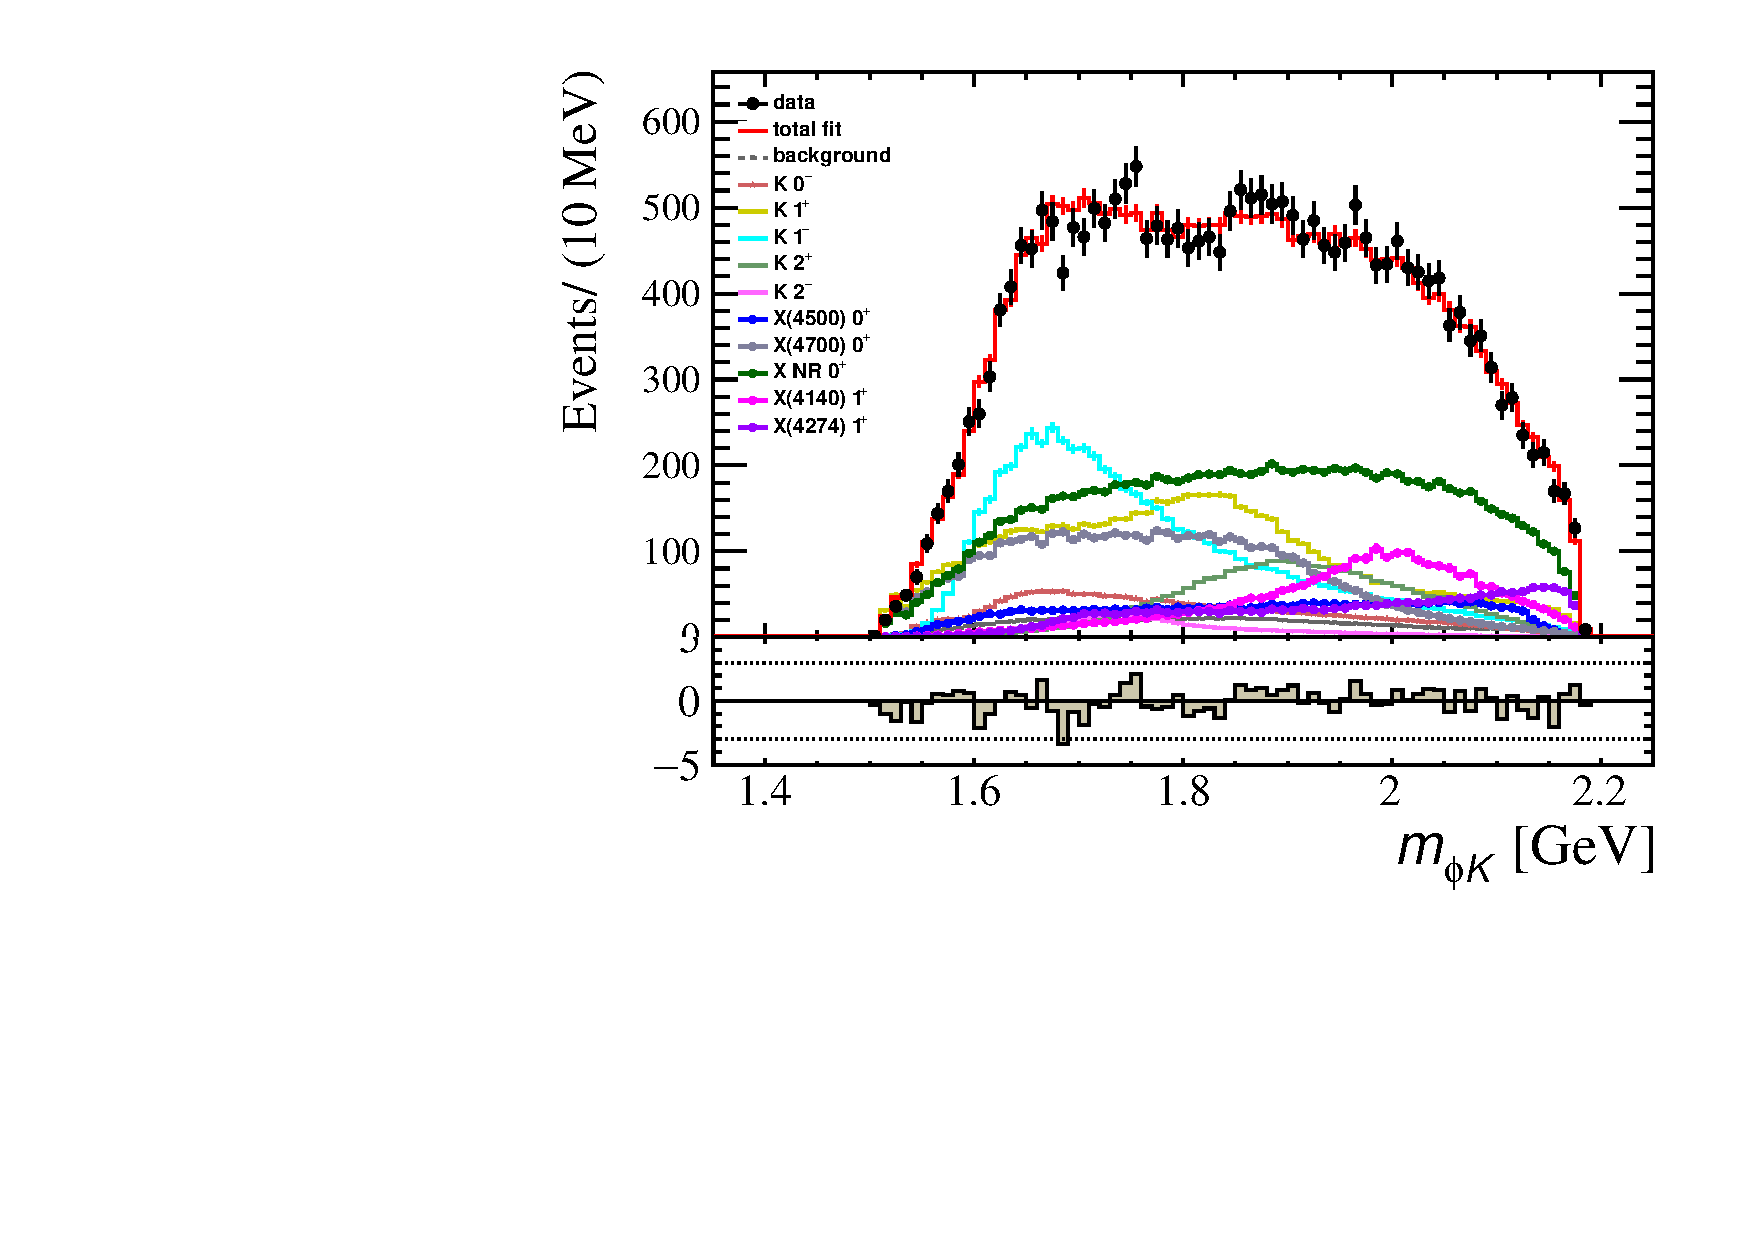
\includegraphics[width=0.6\textwidth]{Figures/03_Zcs/06_Amplitude/fit0/mphik-Test0NoZ}
\put(-60,168) {\textrm{\small \bf(a)}}\\
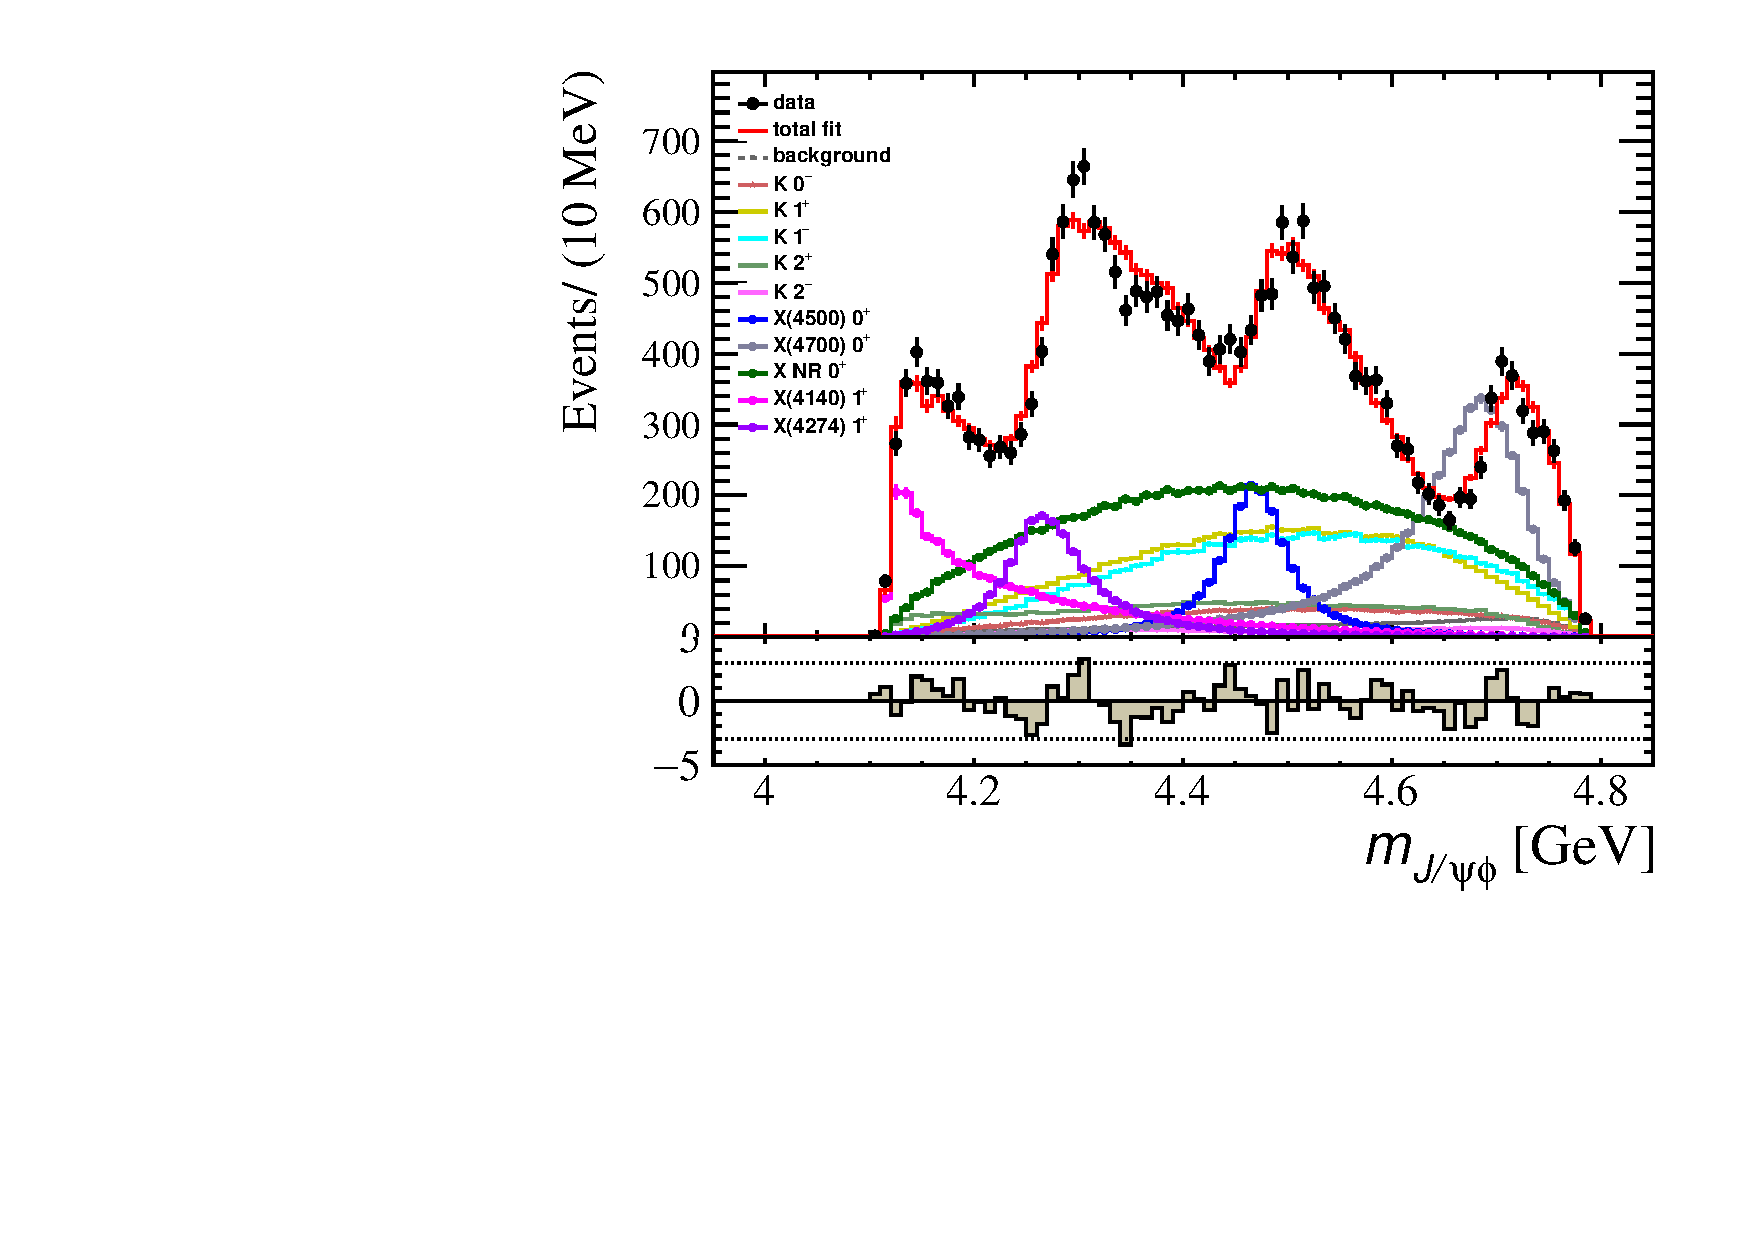
\includegraphics[width=0.6\textwidth]{Figures/03_Zcs/06_Amplitude/fit0/mjpsiphi-Test0NoZ}
\put(-60,168) {\textrm{\small \bf(b)}}\\
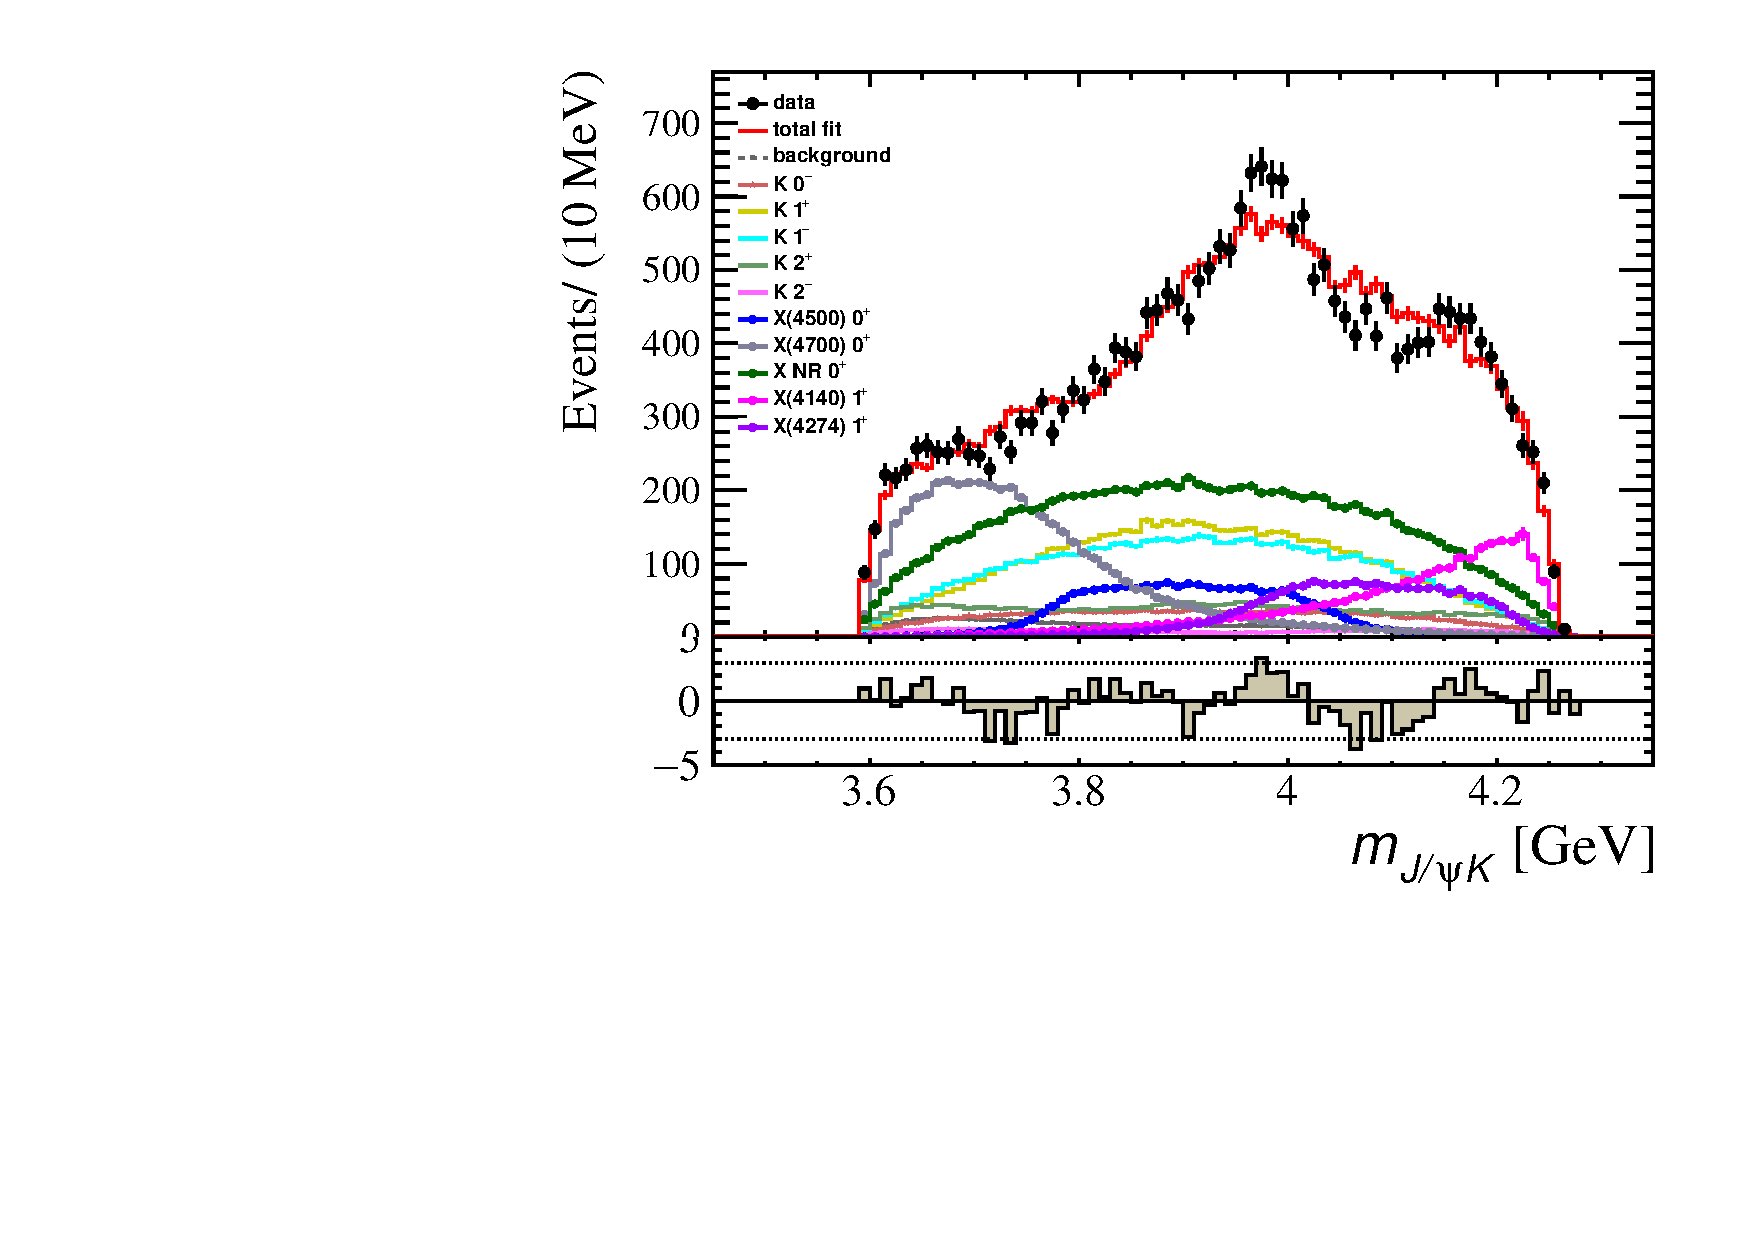
\includegraphics[width=0.6\textwidth]{Figures/03_Zcs/06_Amplitude/fit0/mjpsik-Test0NoZ}
\put(-60,168) {\textrm{\small \bf(c)}}
\caption{Fit projections of (a) $\mfk$, (b) $\mjf$, (c) $\mjk$ by fitting Run 1 model to the new Run 1+2 data sample.}
\label{fit0}
\end{figure}

Then, more drastic changes by adding new exotic hadron components are studied, 
$X$ or $Z_{cs}$ states of different $J^P$ hypotheses.
To ensure that such components are not reflections of inadequacy of our $K^*$ model, 
besides, 
more predicted higher mass $K^*$ resonances is also tried. 
The results from adding one component at a time are listed in Table~\ref{tab:imp},
which shows two states giving the largest likelihood improvements first ($1^+$ $Z_{cs}$ and $1^+$ $X$), 
and then more check,
if any further $X$ or $Z_{cs}$ state significantly improved the model, 
is applied.
In the second iteration, 
several states give large improvements; $1^-$ and $1^+$ $Z_{cs}$ improve $\ln\Like$ by 110 and 104, 
while $1^-$ and $2^-$ $X$ by 100 and 69. 
Since the $1^+$ and $1^-$ $Z_{cs}$ are at about the same mass (4.2\gev), 
they might be the same state. 
Therefore the two $X$ states and one $Z_{cs}$ state are chosen in the third iteration. 
In total, 
three more $X$ and two $Z$ components are added to the model. 
All new states have significances above $5\sigma$, as evaluated by taking them out of the default model one-by-one. 
Further addition of an $X$ state of any $J^P$ gives components with significance below $5\sigma$.


Larger improvement is from addition of the $\nslj{3}{3}{S}{1}$ $K$ candidate state, 
but the fit returns its mass at the upper kinematic limit and a width of more than 1\gev. 
This state and $X(4140)$ state get very large fit fractions, each about 67\%, and strong negative interference fraction between them of $-93\%$.  
This is not physical, 
therefore, 
it is not considered in the nominal fit, 
but instead include it in extended $K$ model.  


\begin{table}[!hbtp]
\centering
\caption{Improvement on $\ln\Like$ by adding one $X$ or $Z$ or $K$ with different $J^P$ hypothesis.}\label{tab:imp}
\begin{tabular}{ccccccc}\hline
$J^P$&$0^+$& $0^-$&$1^+$&$1^-$&$2^+$&$2^-$\\\hline
$X$&25&25&\bf133&\bf 98&64& \bf 81\\
%$Z$& forbidden &46&\bf134&\bf135&30&46\\
$Z_{cs}$&forbidden&36&\bf195&\bf94&41&42\\
\hline\hline
$J^P$&$\nslj{3}{1}{S}{0}(0^-)$& $\nslj{1}{3}{D}{3}(3^-)$&$\nlj{1}{F}{3}(3^+)$&$\nslj{1}{3}{F}{2}(2^+)$&$\nslj{3}{3}{S}{1}(1^-)$\\\hline
$K$&5&18&5&37&70\\
\hline
\end{tabular}
\end{table}


\subsection{Nominal amplitude model}
\label{subsec:nominal}
Based on the investigation described in the previous section, 
the nominal model is now built, 
which includes two $Z_{cs}$ and three new $X$ components in the fit, 
called 9K+5X+3X+2Z model. 
Since additional $K^*$ resonances are not as significant, 
which are used to study systematic uncertainties. 
The second $Z_{cs}$ with $J^P=1^+$  or $1^-$ give similar fit likelihood. 
However the $1^-$ $Z_{cs}$ fit is not very physical, 
because its interference fraction with $X(4140)$ state is $-8.8\%$, 
but its FF is only $8.2\%$, 
and its mass is also at the high mass boundary. 
Instead, 
the $1^+$ $Z_{cs}$ looks more physical, 
therefore,
the $1^+$ $Z$ fit for the nominal model is choosen, 
and use the other one as model variation used to evaluate systematic errors.

The nominal model gives $\ln\Like=5004$, 
about 580 improvement for 45 more free parameters with respect to the 9K+5X model which does not include new exotic hadron components. 
The improvement in $\ln\Like$ is about equal to the sum of individual improvements in Table~\ref{tab:imp}, 
illustrating that the added five exotic states are independent.  

The mass projections are well modelled by the nominal fit as shown in Figure.~\ref{fig:fit5}. 
Two-dimensional Dalitz-plot distributions generated from the nominal amplitude model are shown Figure.~\ref{fig:sec5_dalitz_plot}. 
The data structures in Figures.~\ref{fig:dp1}-\ref{fig:dp3} are well reproduced.  
Figure.~\ref{fig:fitmjpsik} shows the $\mjk$ distributions in two slices of $\mjf$, 
as well as  the overall $\mjk$ projection without the two $1^+$ $Z_{cs}$ states included in Figure.~\ref{fig:fitmjpsik-noz}. 
The low mass $1^+$ $Z$ at about 4\gev is evident. 
The angular distributions in $\phi K$ decay chain are shown in Figure.~\ref{fig:ang}. 
They are well described by the nominal fit. 

Fit results are shown in Table~\ref{tab:fit}, 
including masses, widths, fit fractions, and significance of each component. 
The significance of each component is evaluated by assuming that the change of $2\ln\Like$ between the default fit and the fit without this component, 
obeys the $\chi^2$ distribution with number of degrees of freedom (ndf) equal to twice the reduction in number of free parameters, 
to take into account look elsewhere effect \supercite{LHCb-PAPER-2016-019}. 
The ndf is not multiplied by two for the $K^*$ resonance whose mass and width are fixed. 
All the included states are above 5$\sigma$ significant. 
The statistical significance for two $Z_{cs}$ states are 16 and 8\,$\sigma$, respectively. 
Three new $X$ states are 15, 8.7 and 5.7\,$\sigma$ significant, respectively.


\begin{figure}[!tbp]
\centering
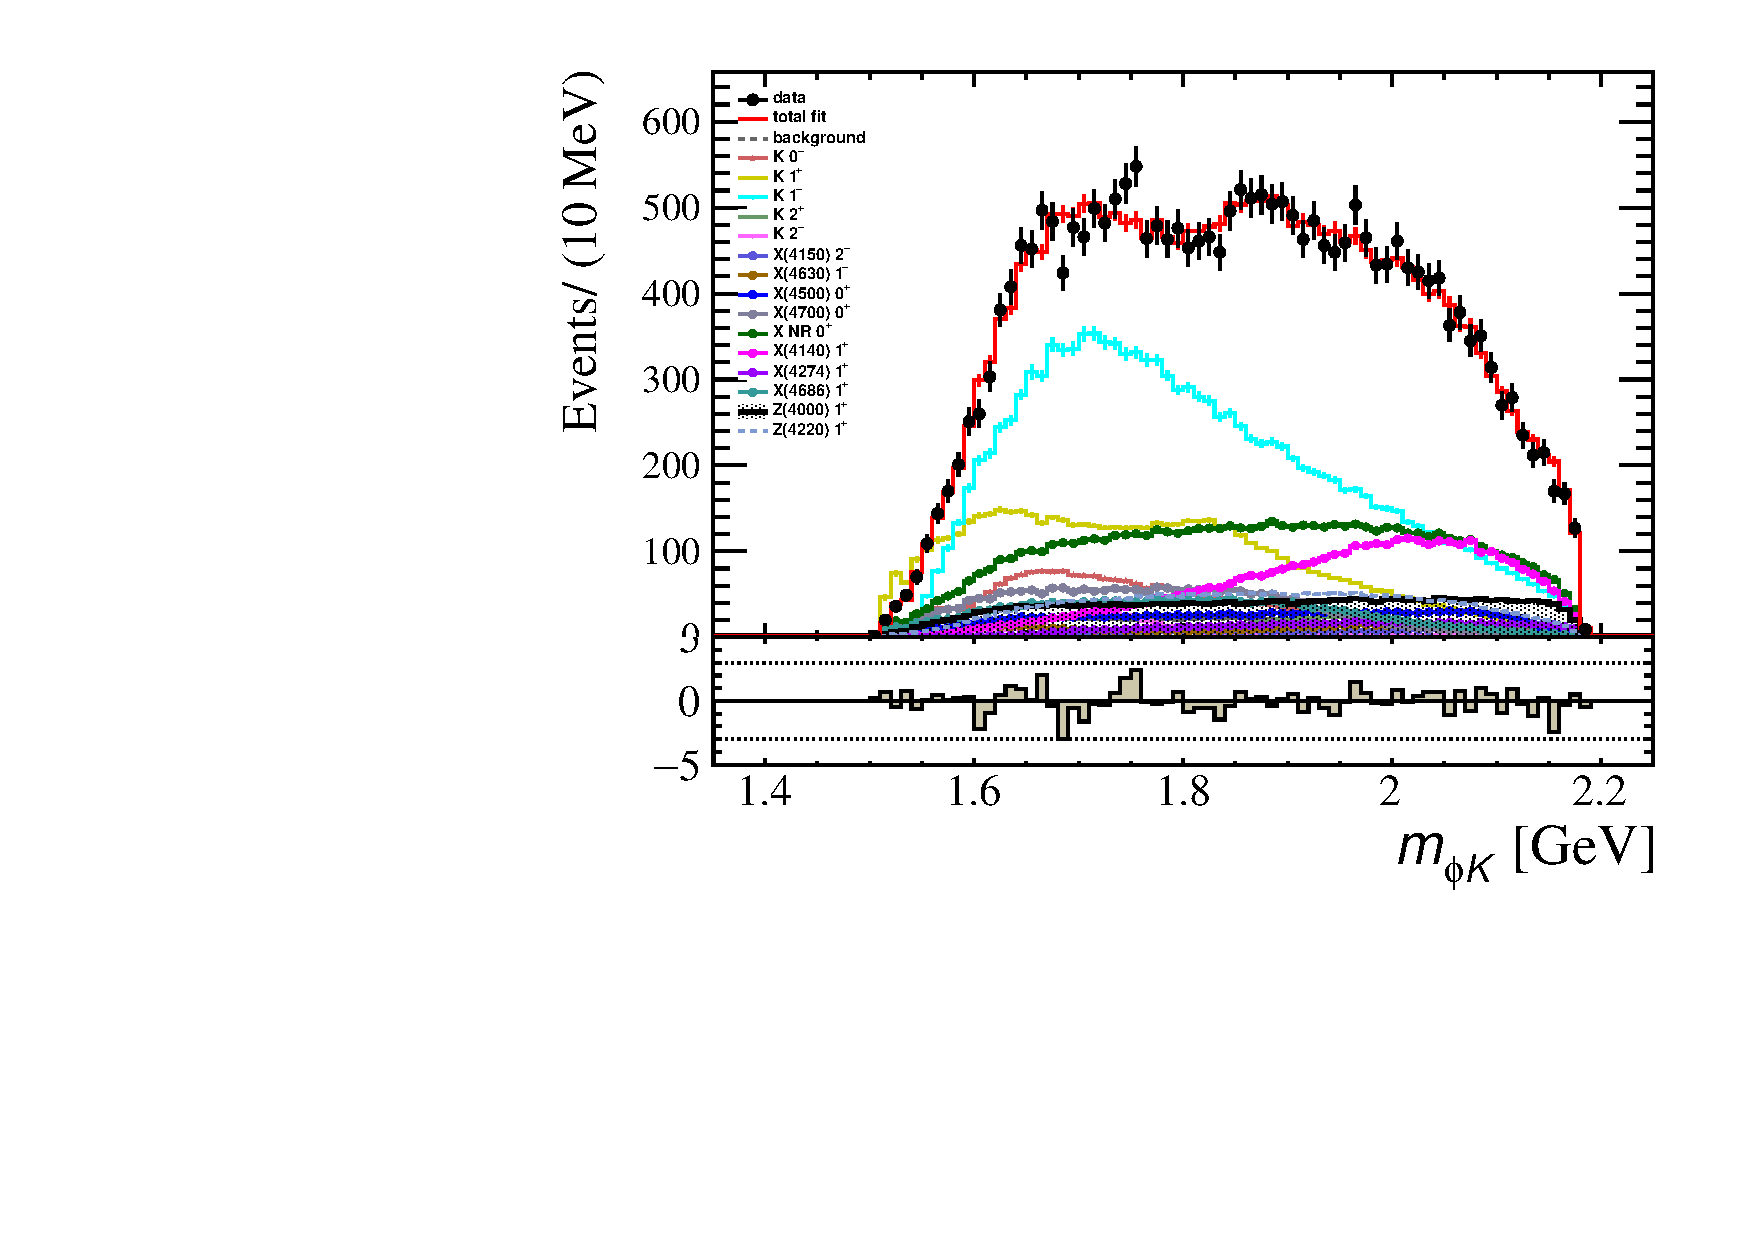
\includegraphics[width=0.6\textwidth]{Figures/03_Zcs/06_Amplitude/fitx2m/mphik-X2mZ1P} 
\put(-60,168) {\textrm{\small \bf(a)}}\\
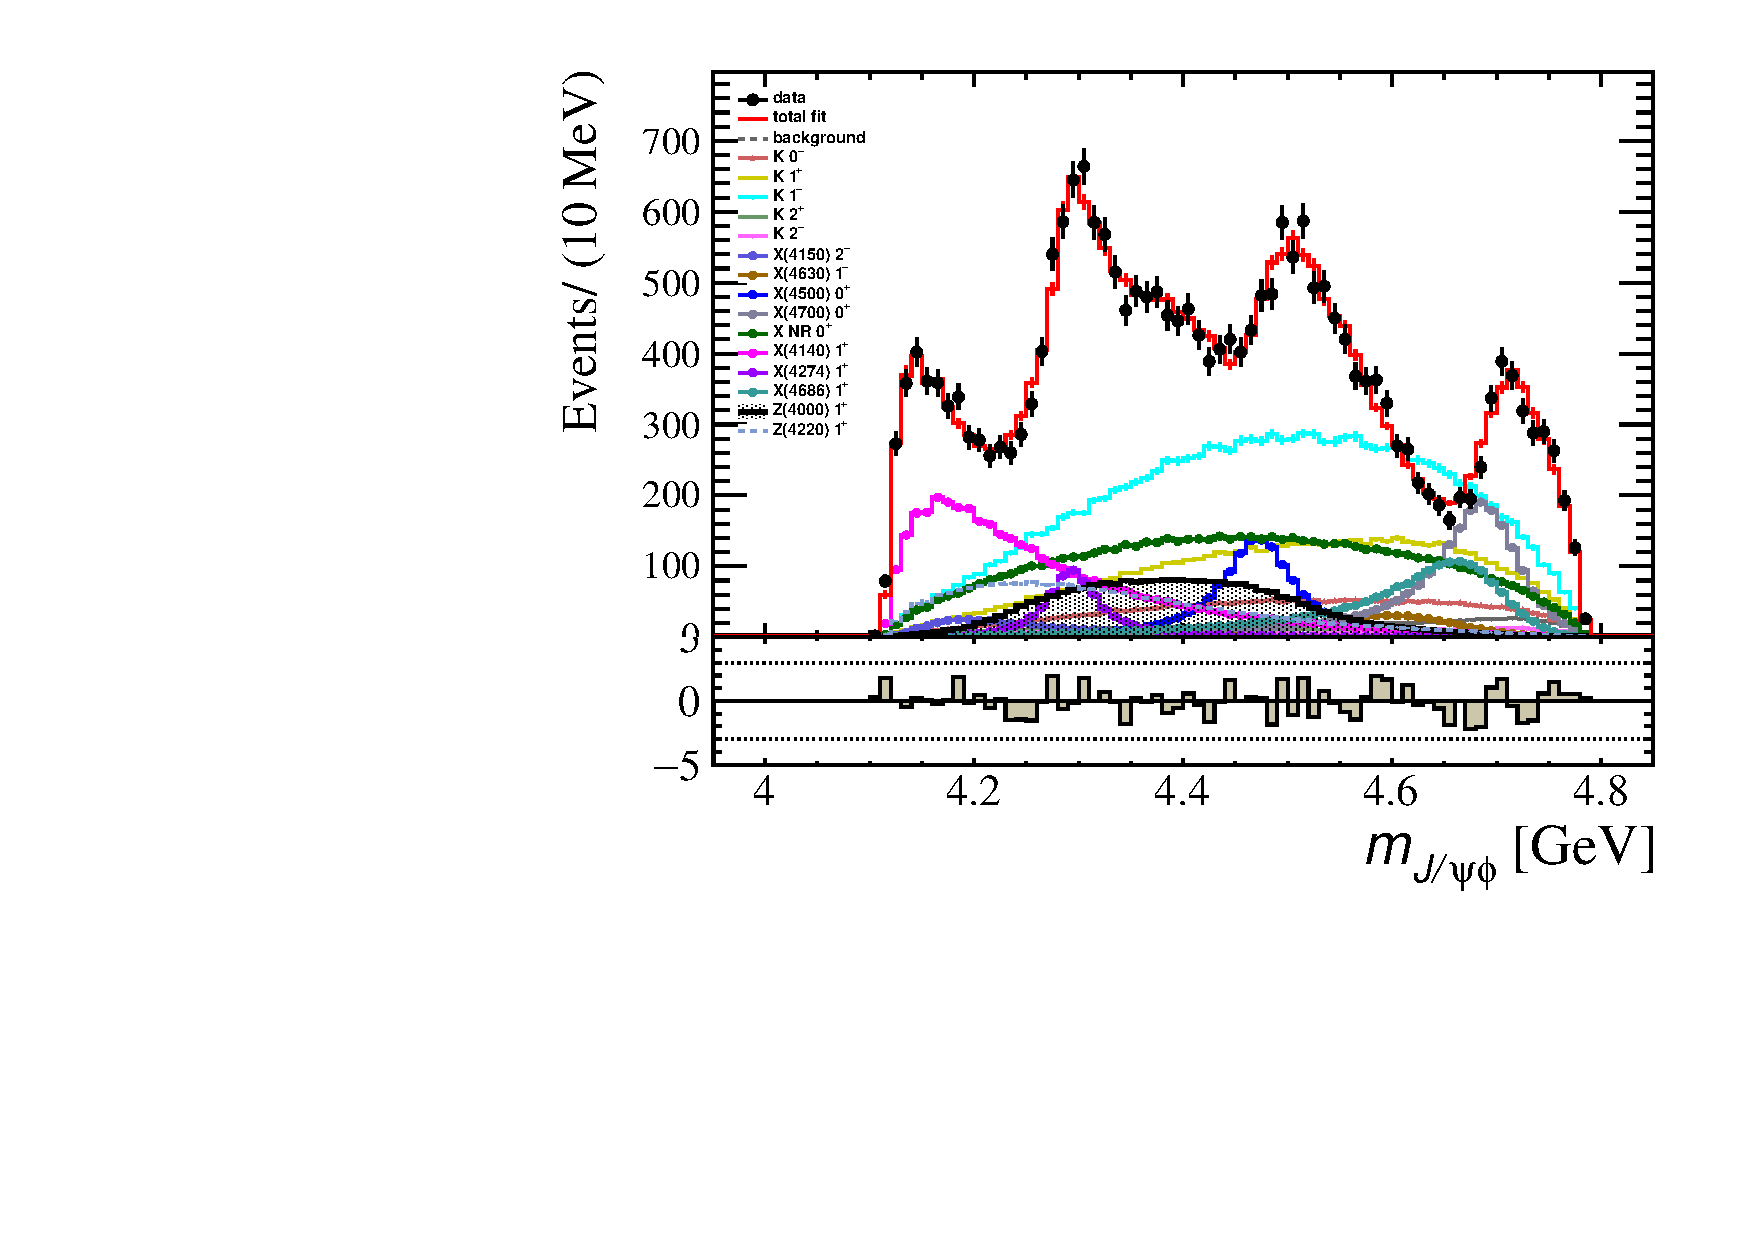
\includegraphics[width=0.6\textwidth]{Figures/03_Zcs/06_Amplitude/fitx2m/mjpsiphi-X2mZ1P}
\put(-60,168) {\textrm{\small \bf(b)}}\\
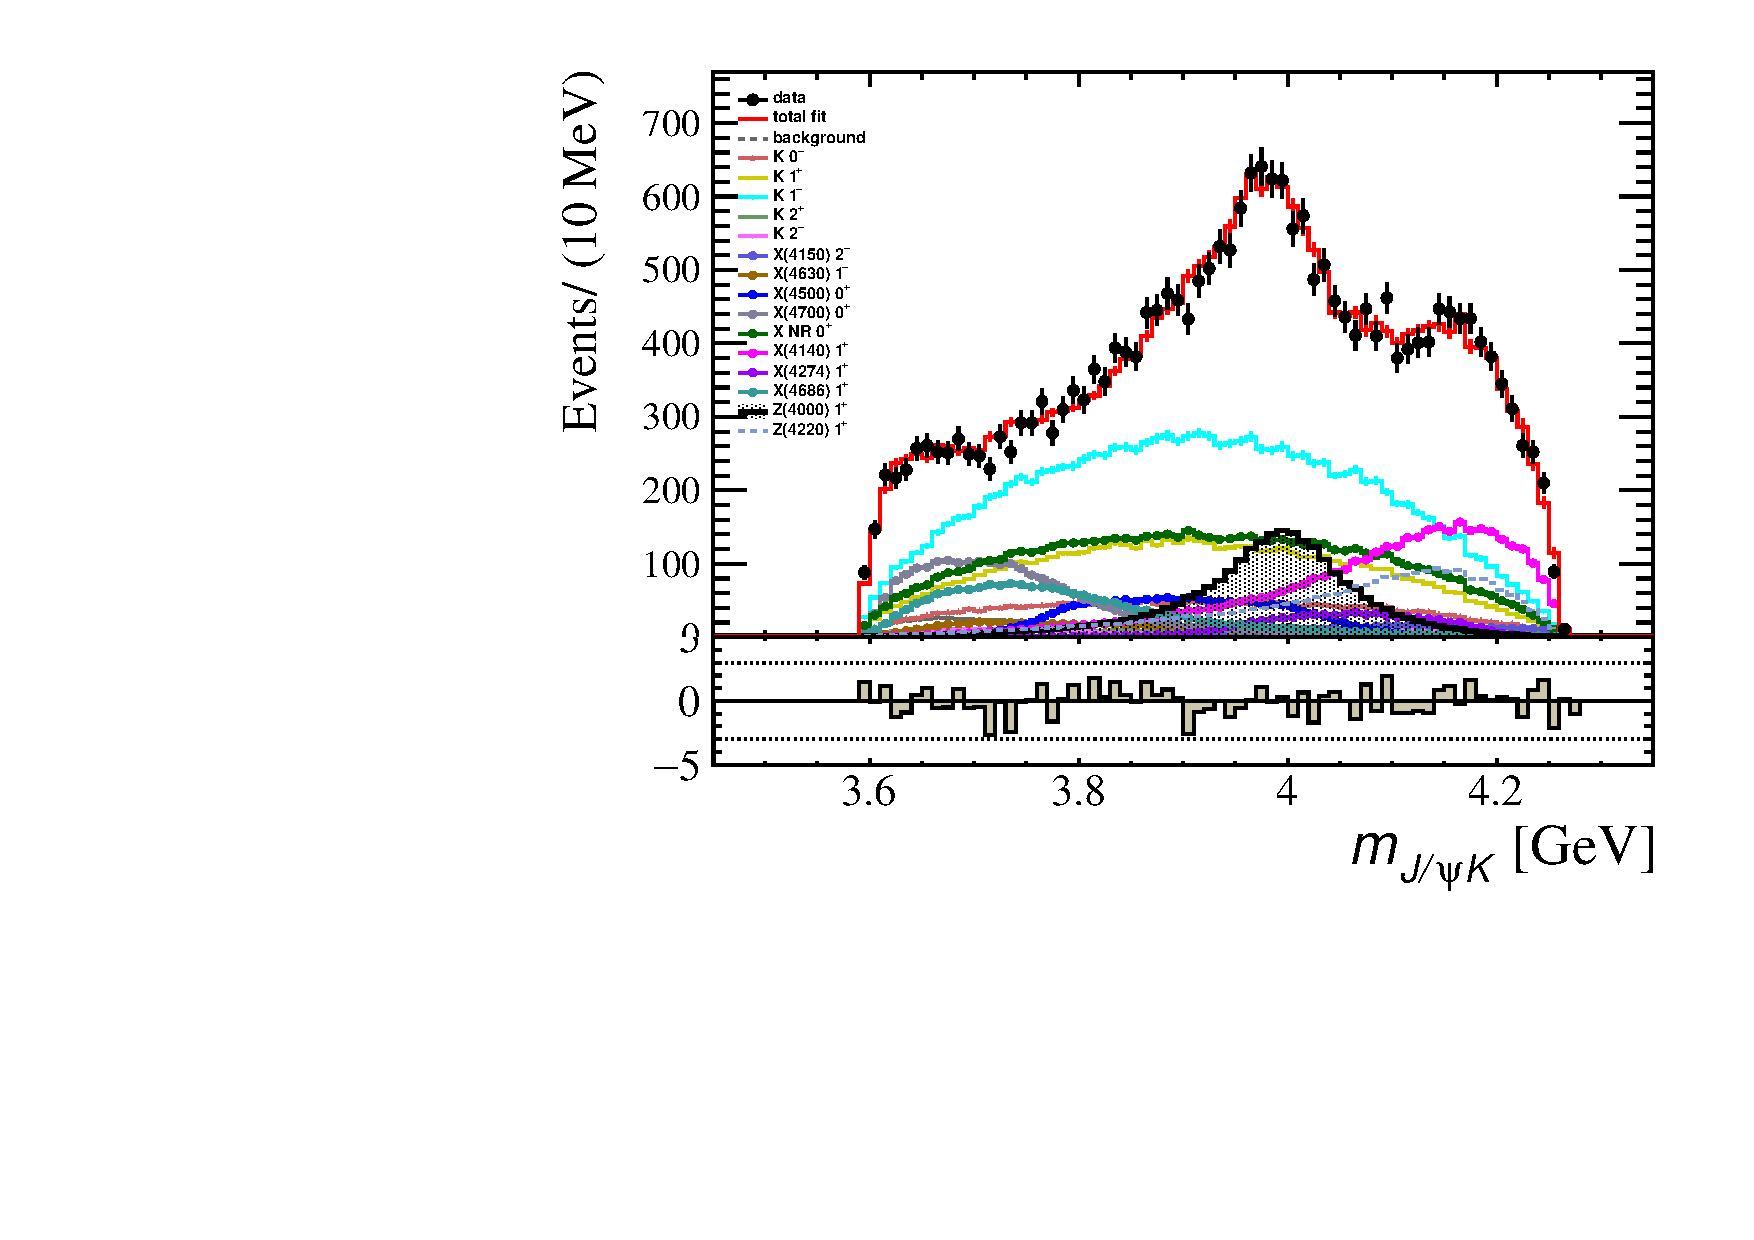
\includegraphics[width=0.6\textwidth]{Figures/03_Zcs/06_Amplitude/fitx2m/mjpsik-X2mZ1P}
\put(-60,168) {\textrm{\small \bf(c)}}
\caption{Fit projections of (a) $\mfk$, (b) $\mjf$, (c) $\mjk$ from the 9K+5X+2X+2Z model.}
\label{fig:fit5}
\end{figure}


\begin{figure}[!tbp]
\centering
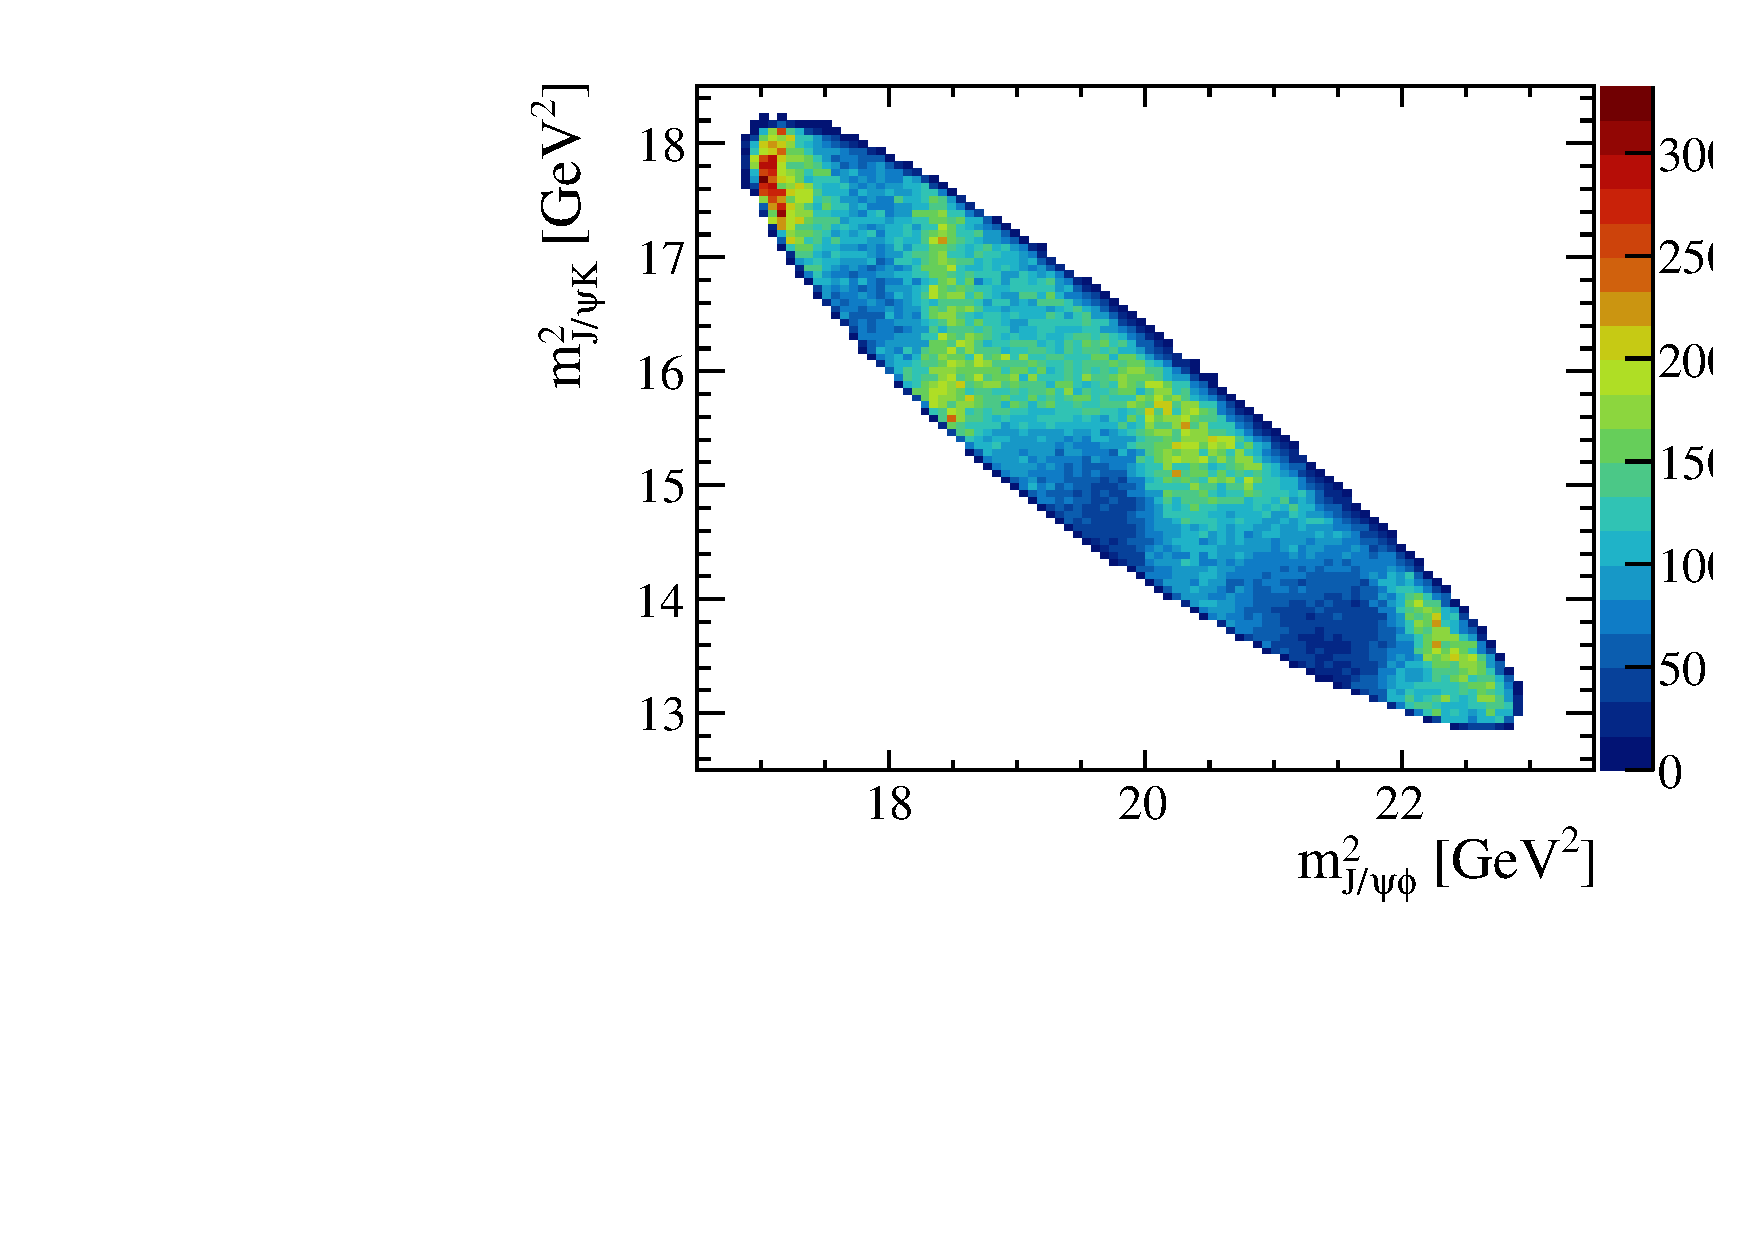
\includegraphics[width=0.6\textwidth]{Figures/03_Zcs/06_Amplitude/dalitz/toy/mjpsik2_mjpsiphi2}
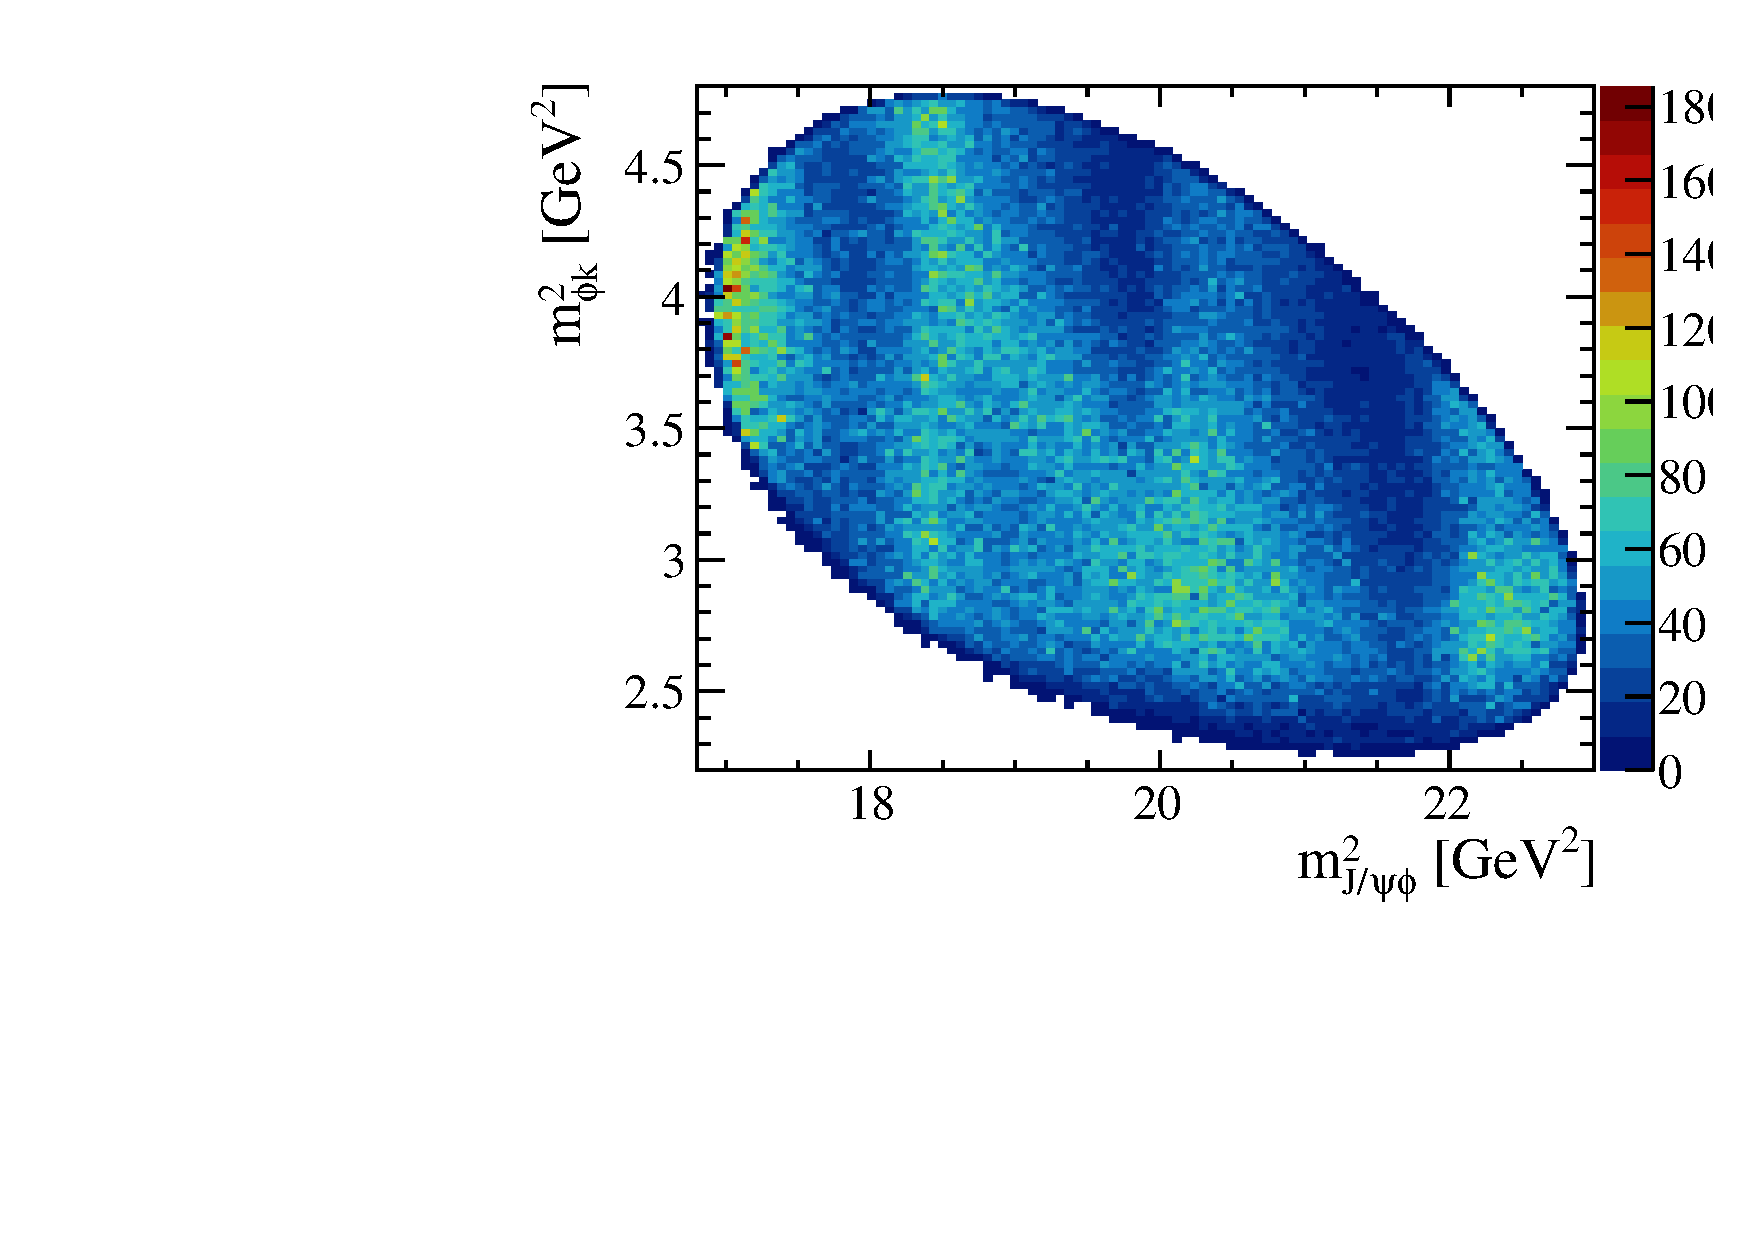
\includegraphics[width=0.6\textwidth]{Figures/03_Zcs/06_Amplitude/dalitz/toy/mphik2_mjpsiphi2}
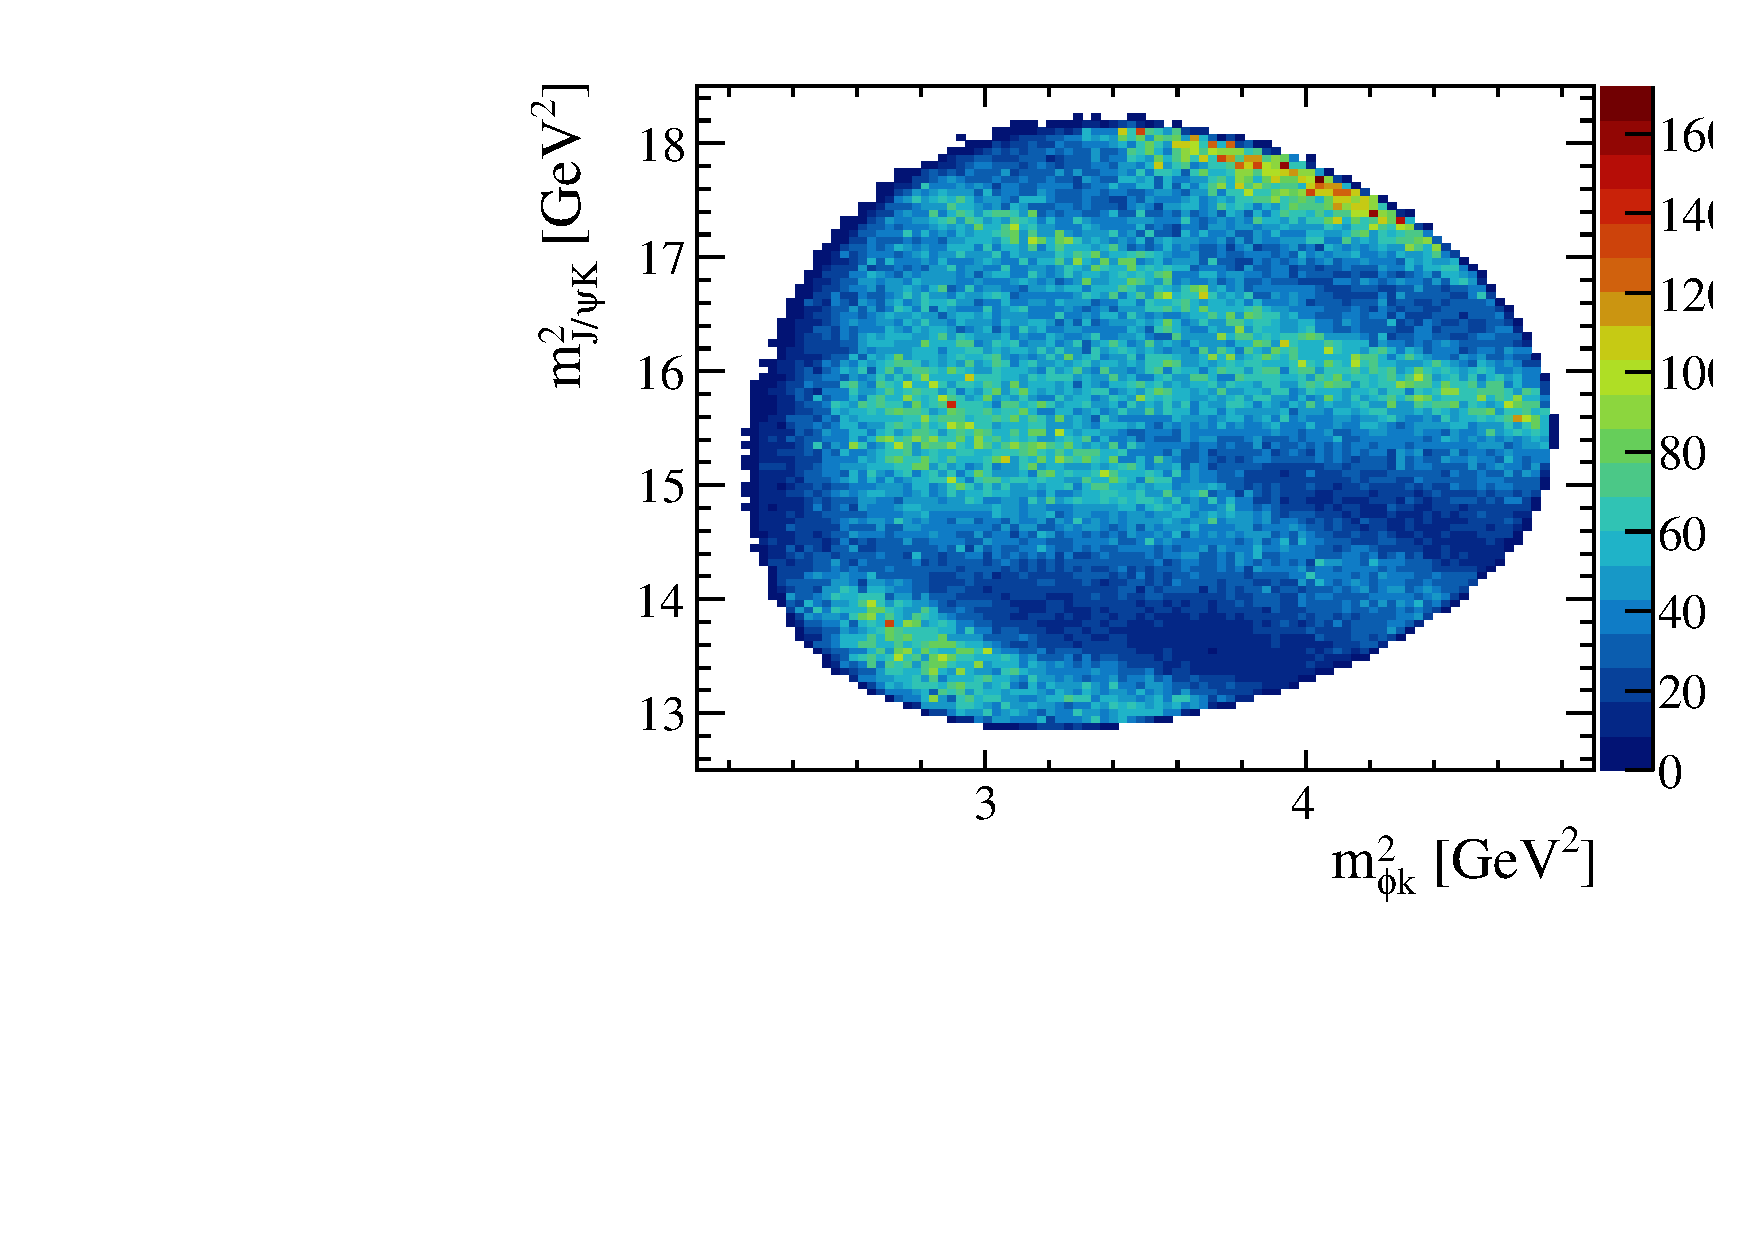
\includegraphics[width=0.6\textwidth]{Figures/03_Zcs/06_Amplitude/dalitz/toy/mjpsik2_mphik2}
\caption{Dalitz-plot distributions of signal from the nominal fit model.}
\label{fig:sec5_dalitz_plot}
\end{figure}


\begin{figure}[!tbp]
\centering
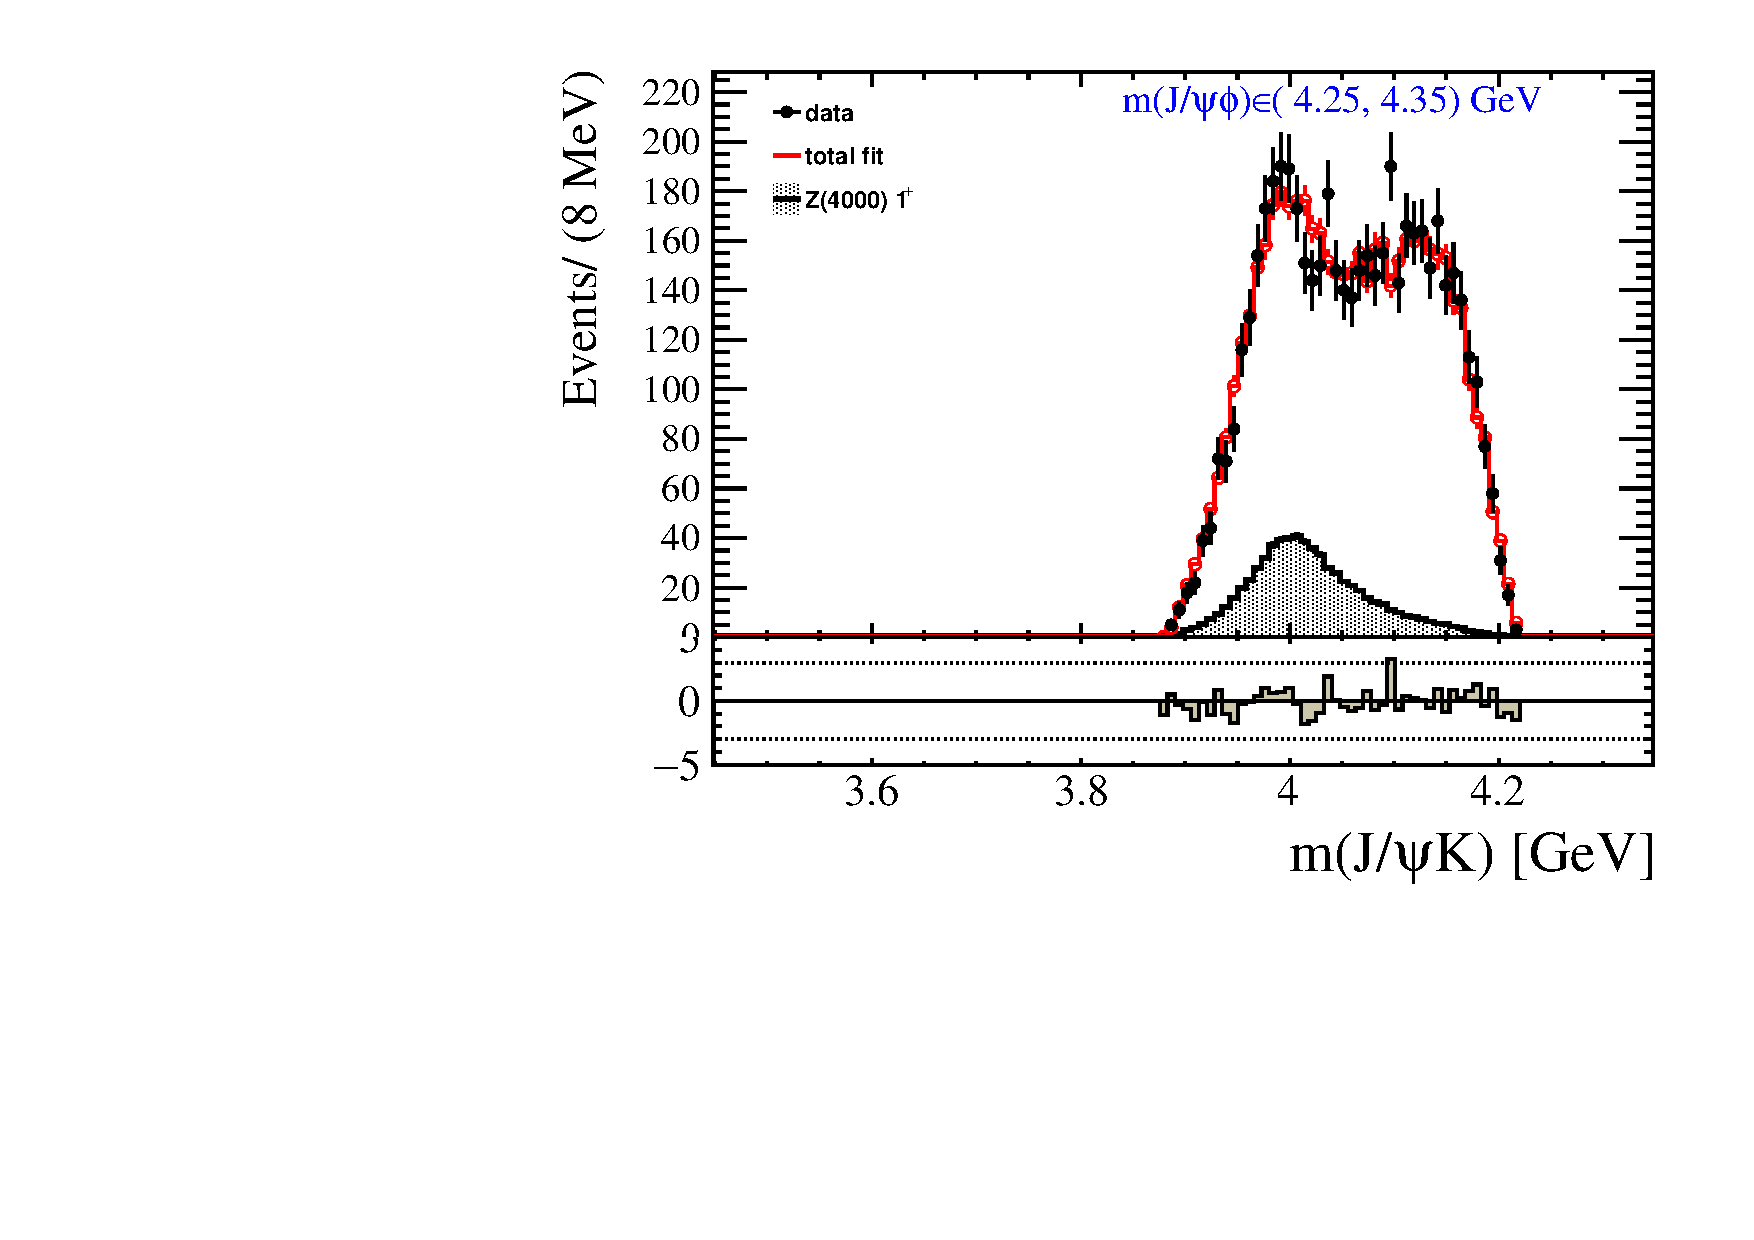
\includegraphics[width=0.5\textwidth]{Figures/03_Zcs/06_Amplitude/fitx2m/mjpsik-1}%
\put(-160,110) {\textrm{\small \bf(a)}}
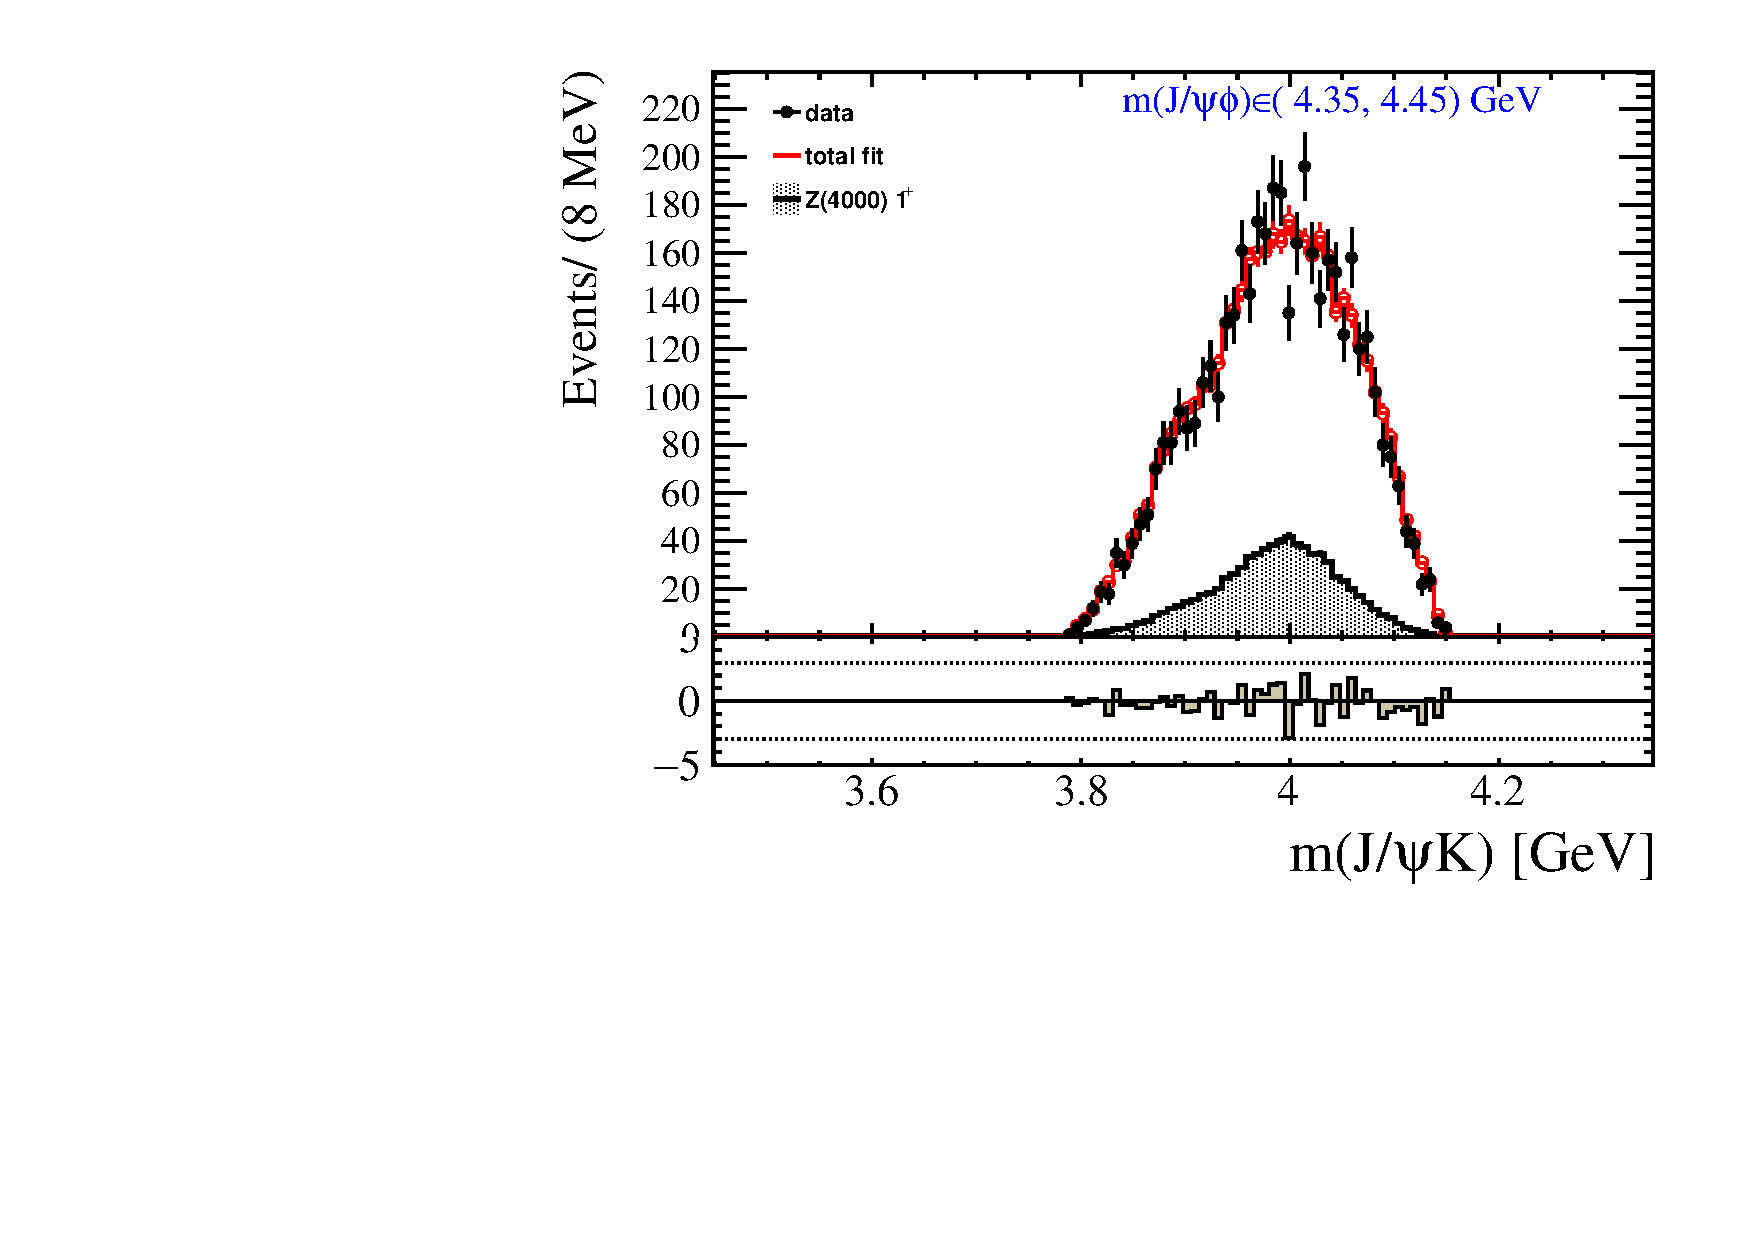
\includegraphics[width=0.5\textwidth]{Figures/03_Zcs/06_Amplitude/fitx2m/mjpsik-2}
\put(-160,110) {\textrm{\small \bf(b)}}\\
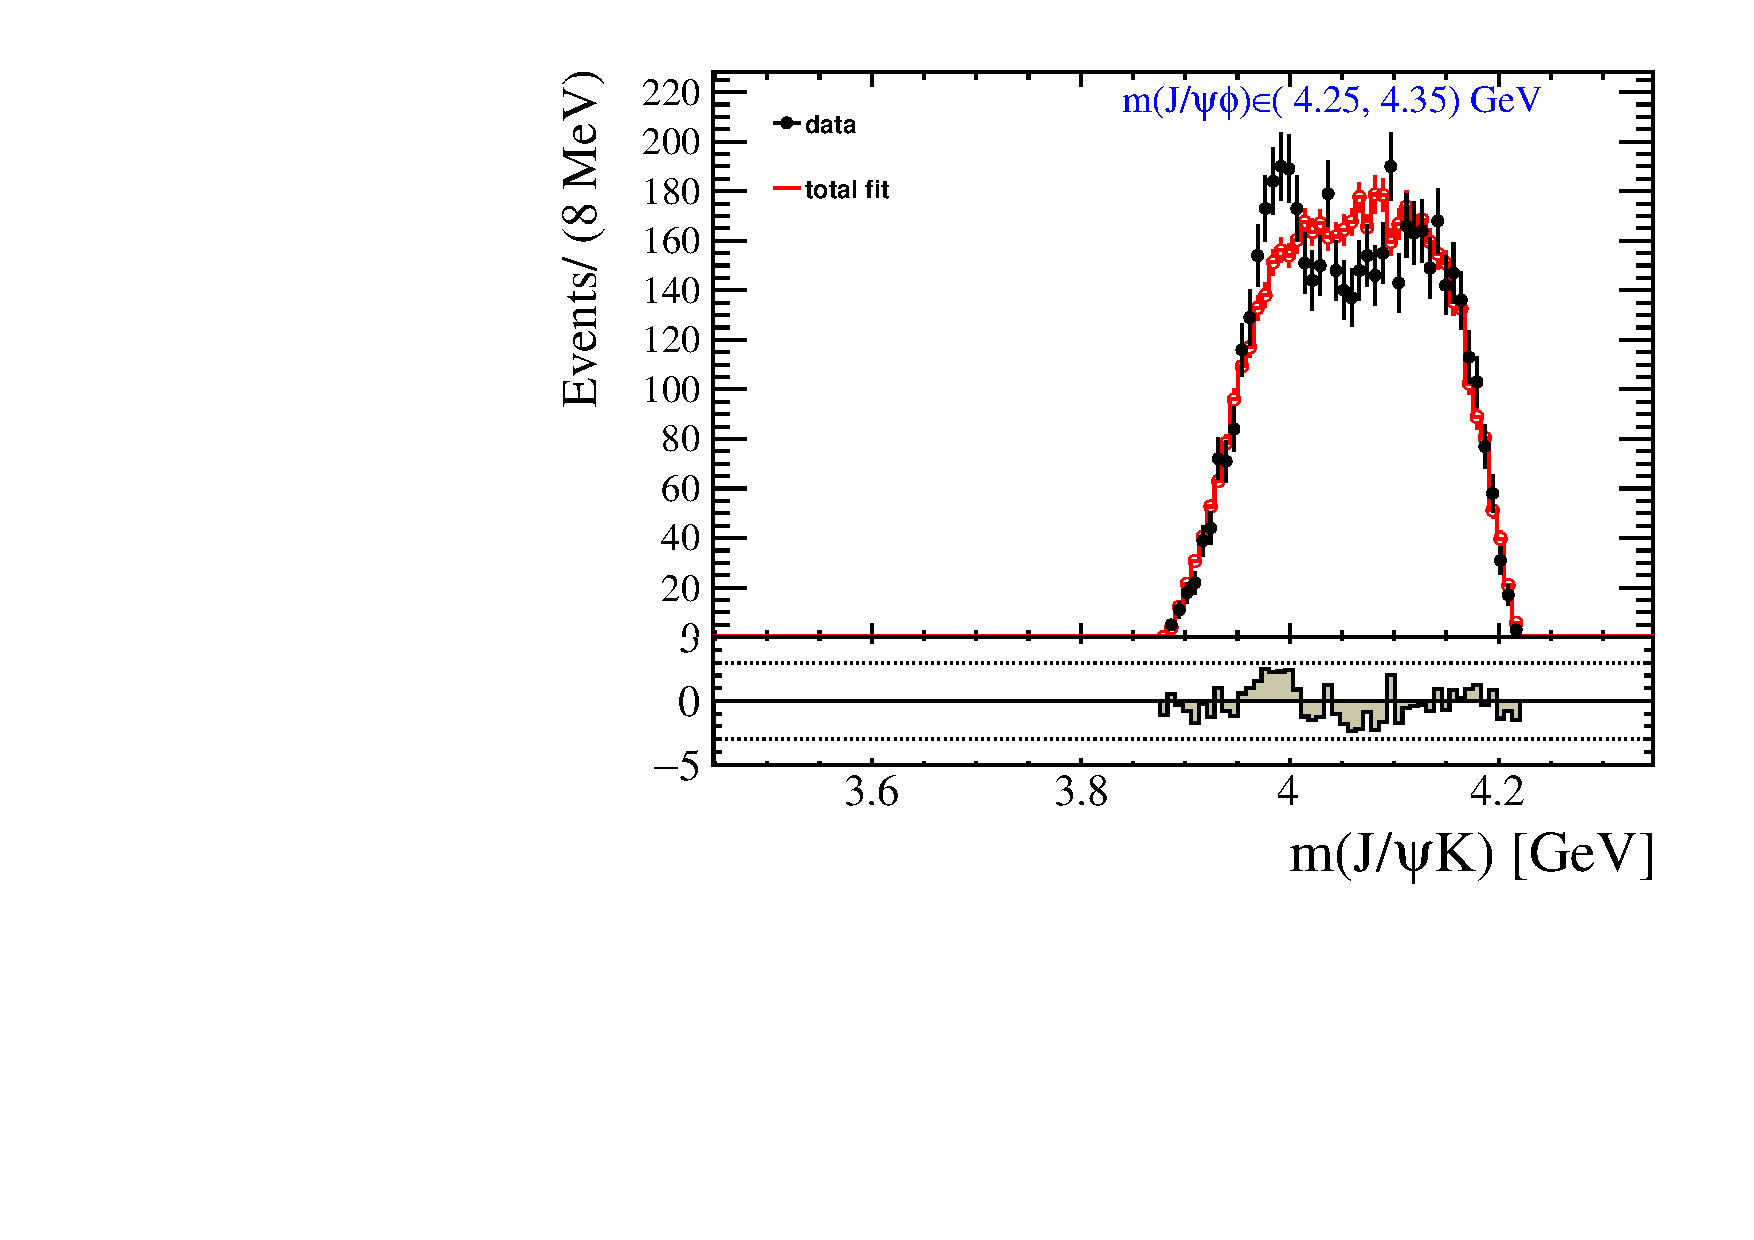
\includegraphics[width=0.5\textwidth]{Figures/03_Zcs/06_Amplitude/fit0/mjpsik-1}%
\put(-160,110) {\textrm{\small \bf(c)}}
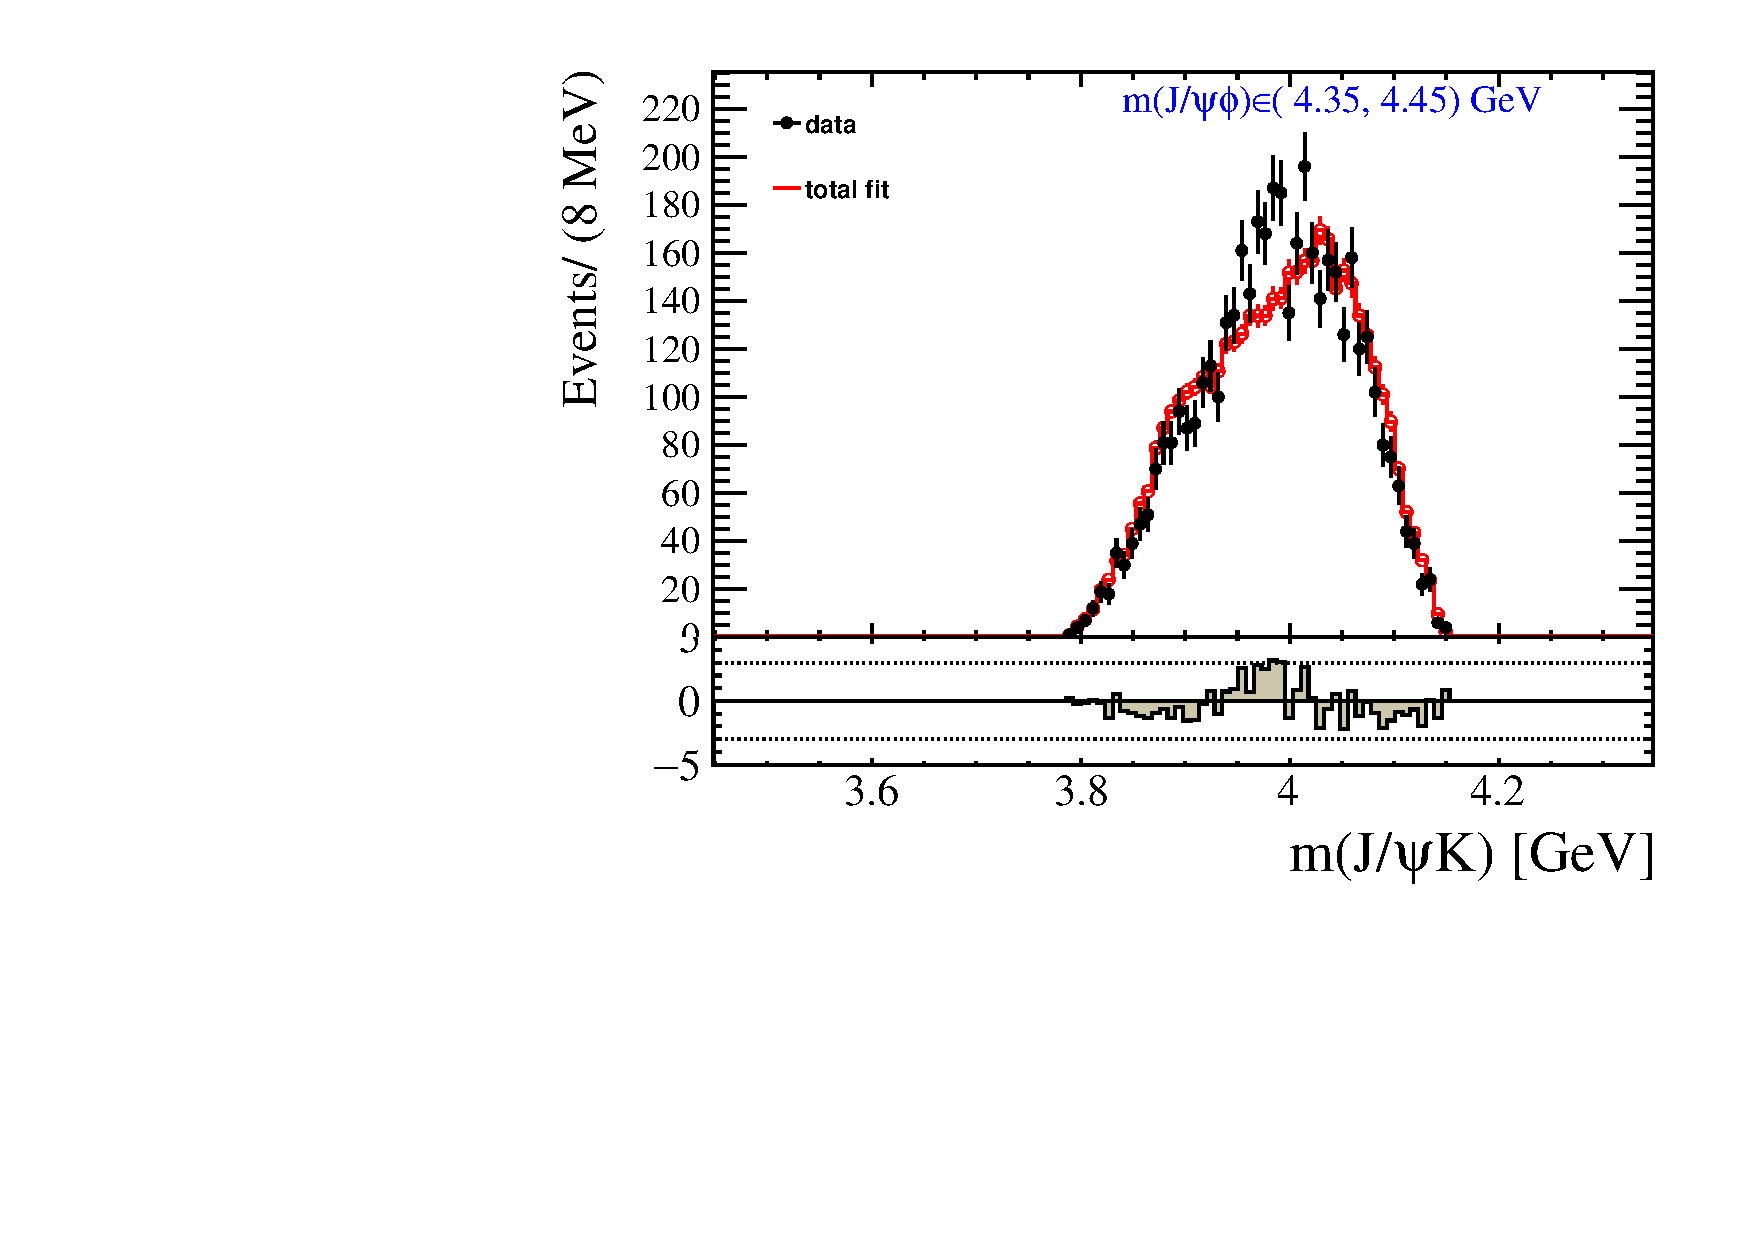
\includegraphics[width=0.5\textwidth]{Figures/03_Zcs/06_Amplitude/fit0/mjpsik-2}
\put(-160,110) {\textrm{\small \bf(d)}} \\
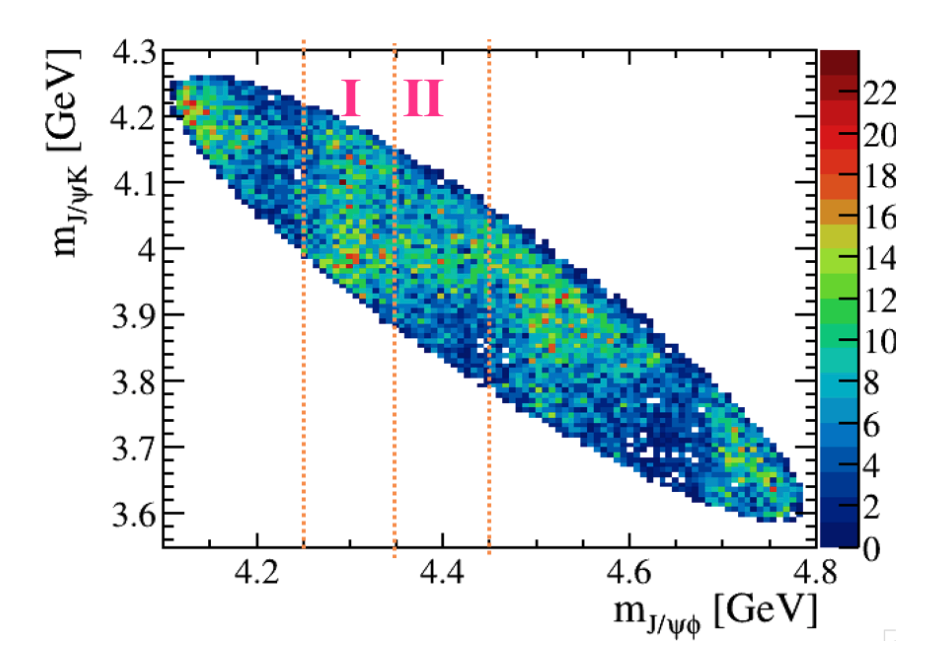
\includegraphics[width=0.5\textwidth]{Figures/03_Zcs/06_Amplitude/Dalitz-band2.png}
\caption{Fit projections of $\mjk$ in two slices of $\mjf$ from the nominal model (top) and the nominal model without $1^+$ $Z_{cs}$ (bottom). 
The narrow $Z_{cs}$ is evident in the two $\mjf$ slices.  
Including $1^+$ $Z_{cs}$ improve the $\chi^2/{\rm nbin}$ from 85/46 to 48/46 (left slice), 
and from 97/49 to 47/49 (right slice). 
Bottom figure shows the two slices of $\mjf$ regions.}
\label{fig:fitmjpsik}
\end{figure}

\begin{figure}[!tbp]
\centering
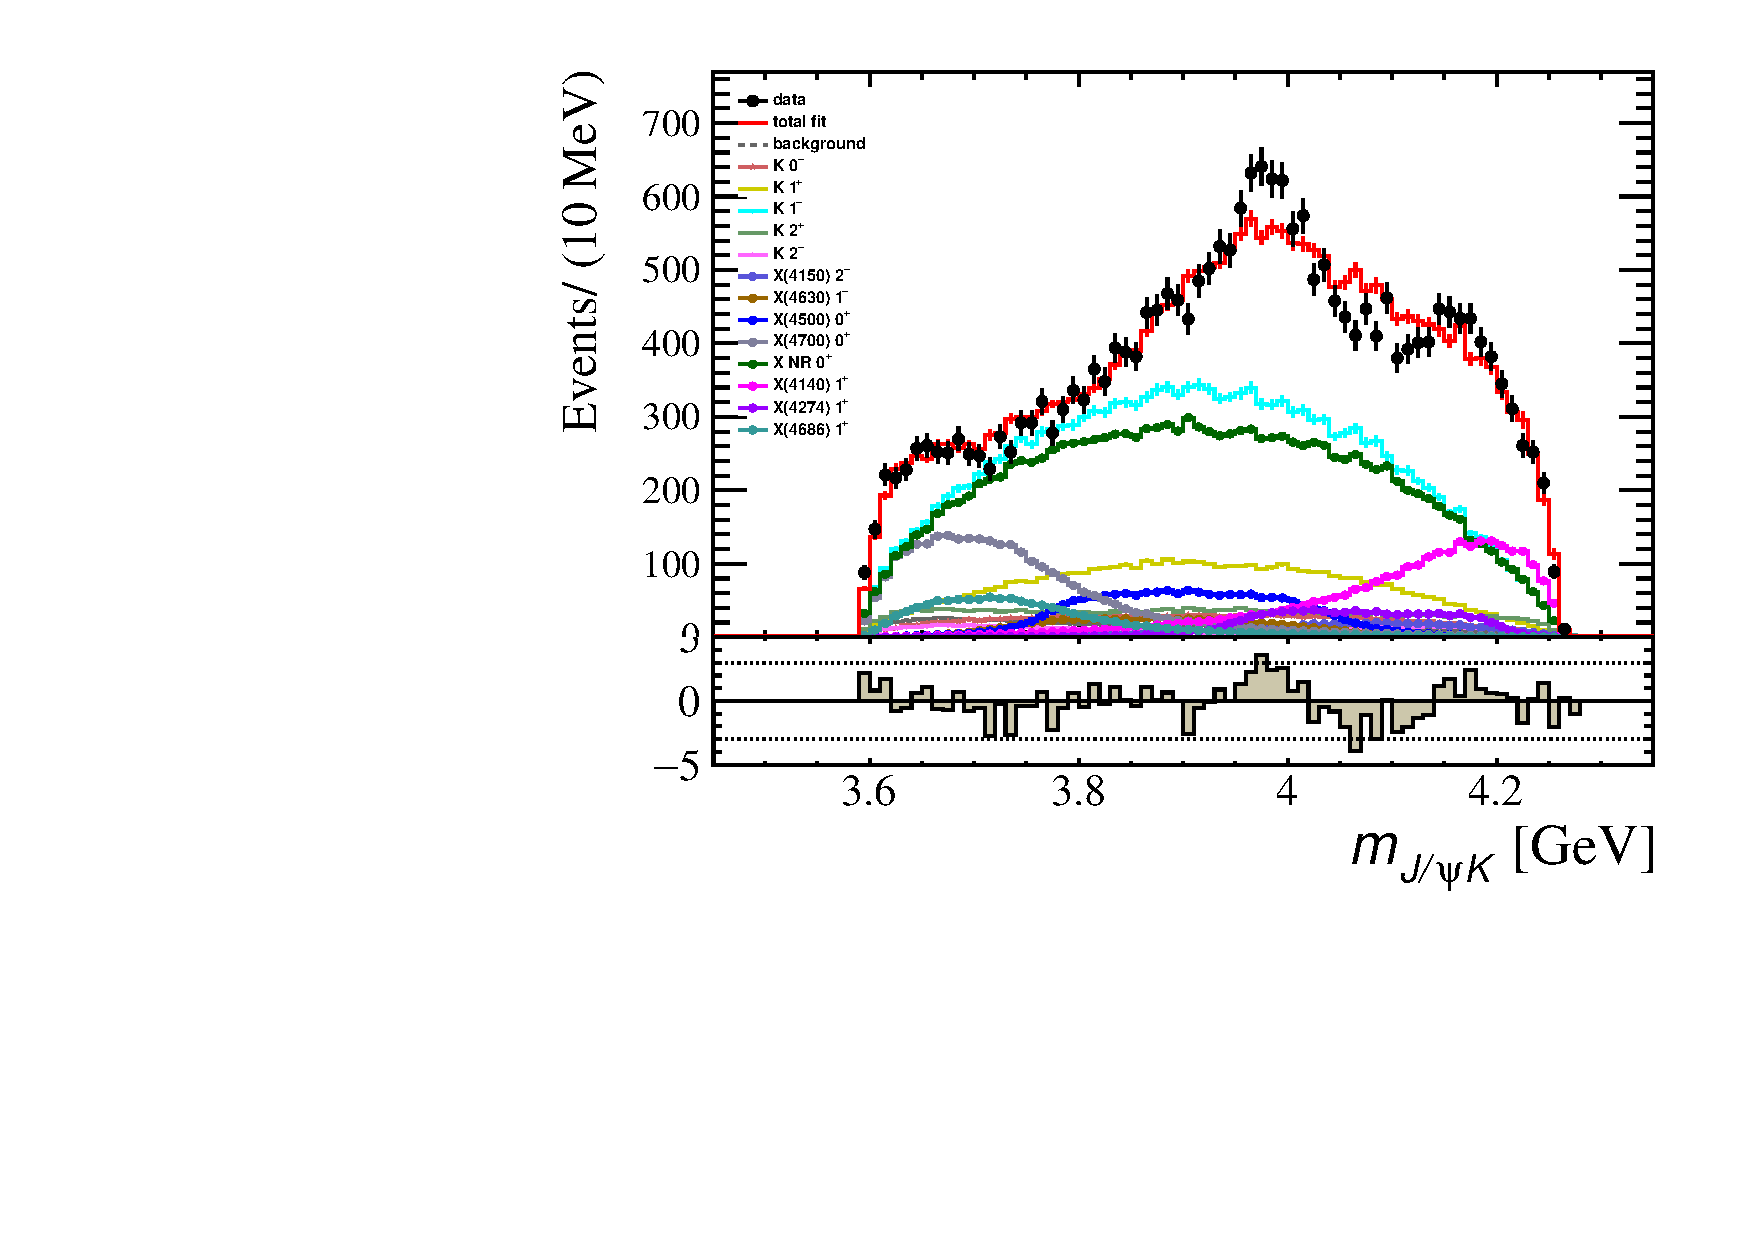
\includegraphics[width=0.6\textwidth]{Figures/03_Zcs/06_Amplitude/fit0/mjpsik-NoZ}%
\caption{Fit projections of $\mjk$ from the nominal model without $1^+$ $Z_{cs}$. }
\label{fig:fitmjpsik-noz}
\end{figure}

\begin{figure}[!tbp]
\centering
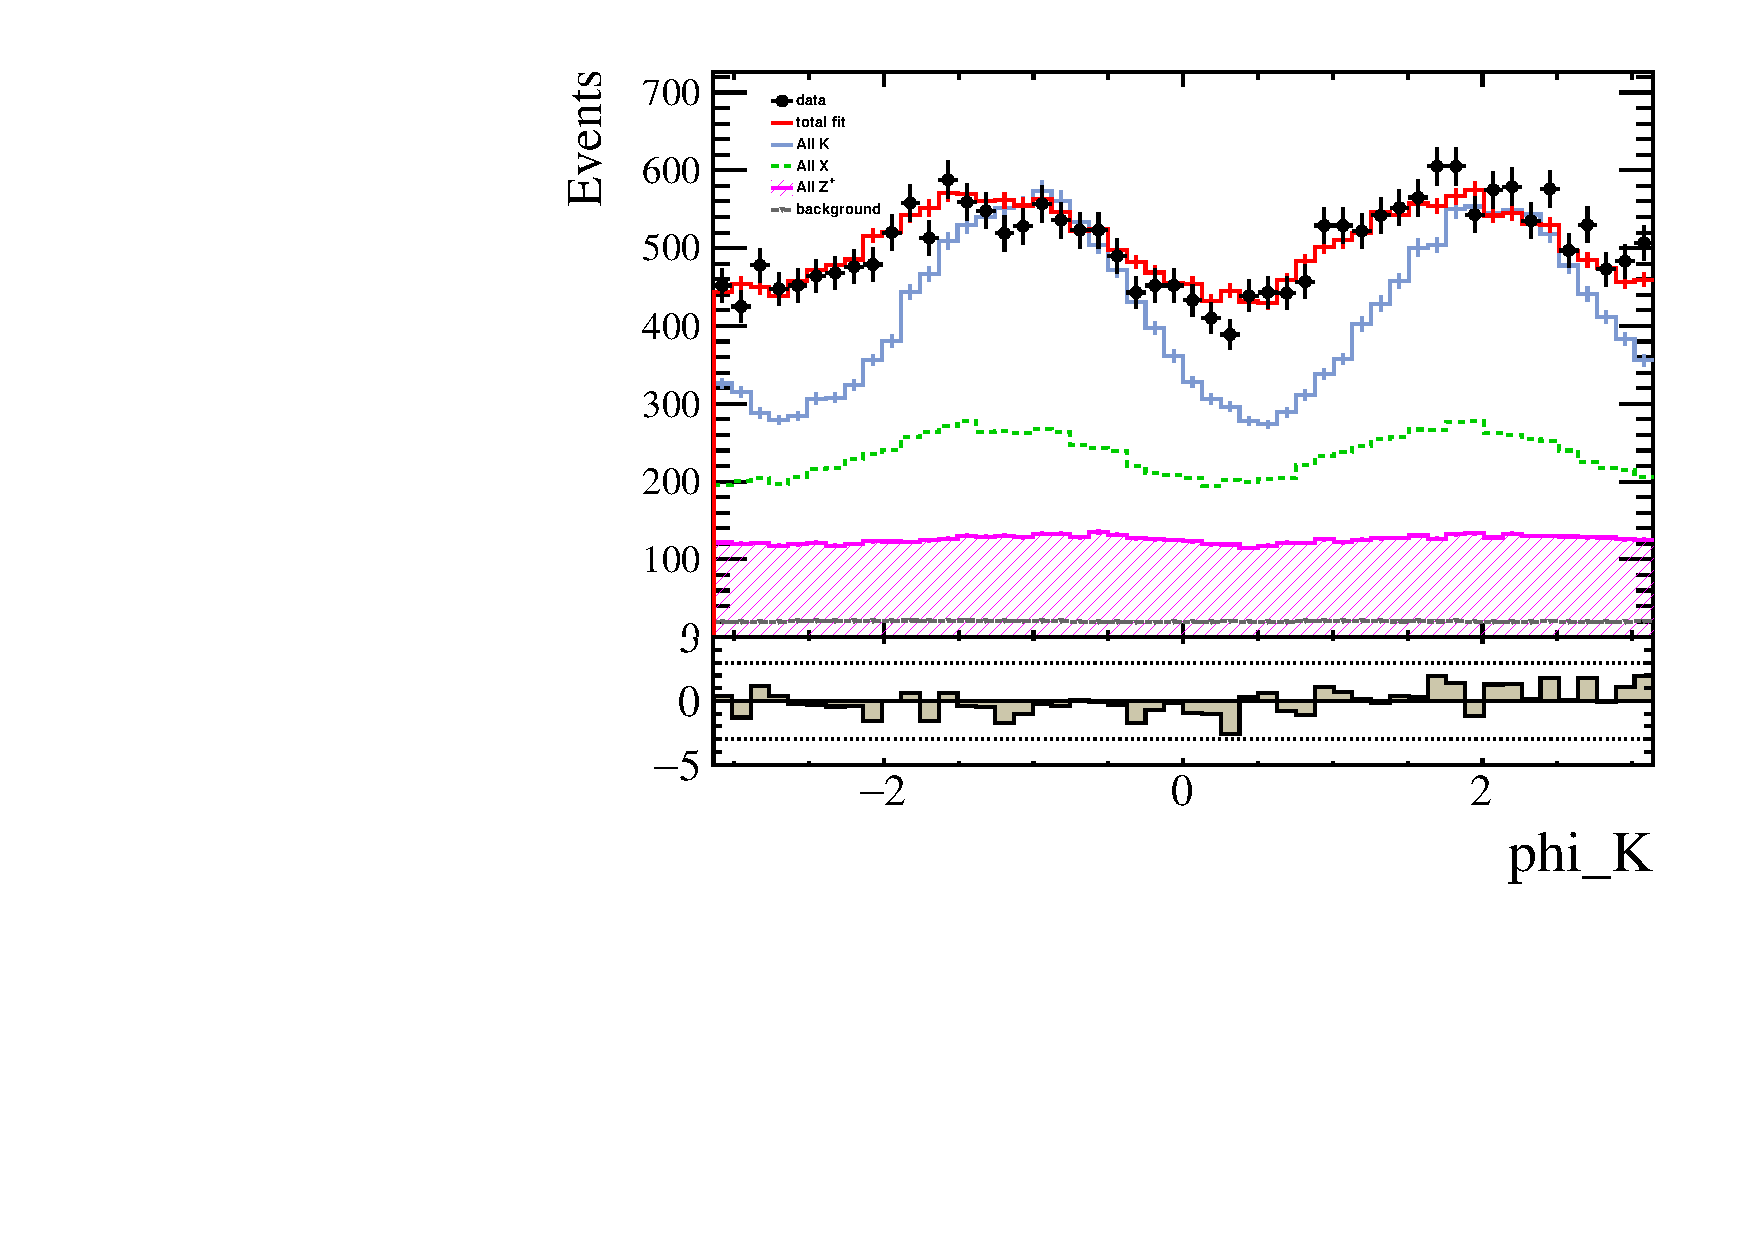
\includegraphics[width=0.5\textwidth]{Figures/03_Zcs/06_Amplitude/fitx2m/phi_K}%
\put(-80,145) {\textrm{\small \bf(a) $\phiksphi$}}
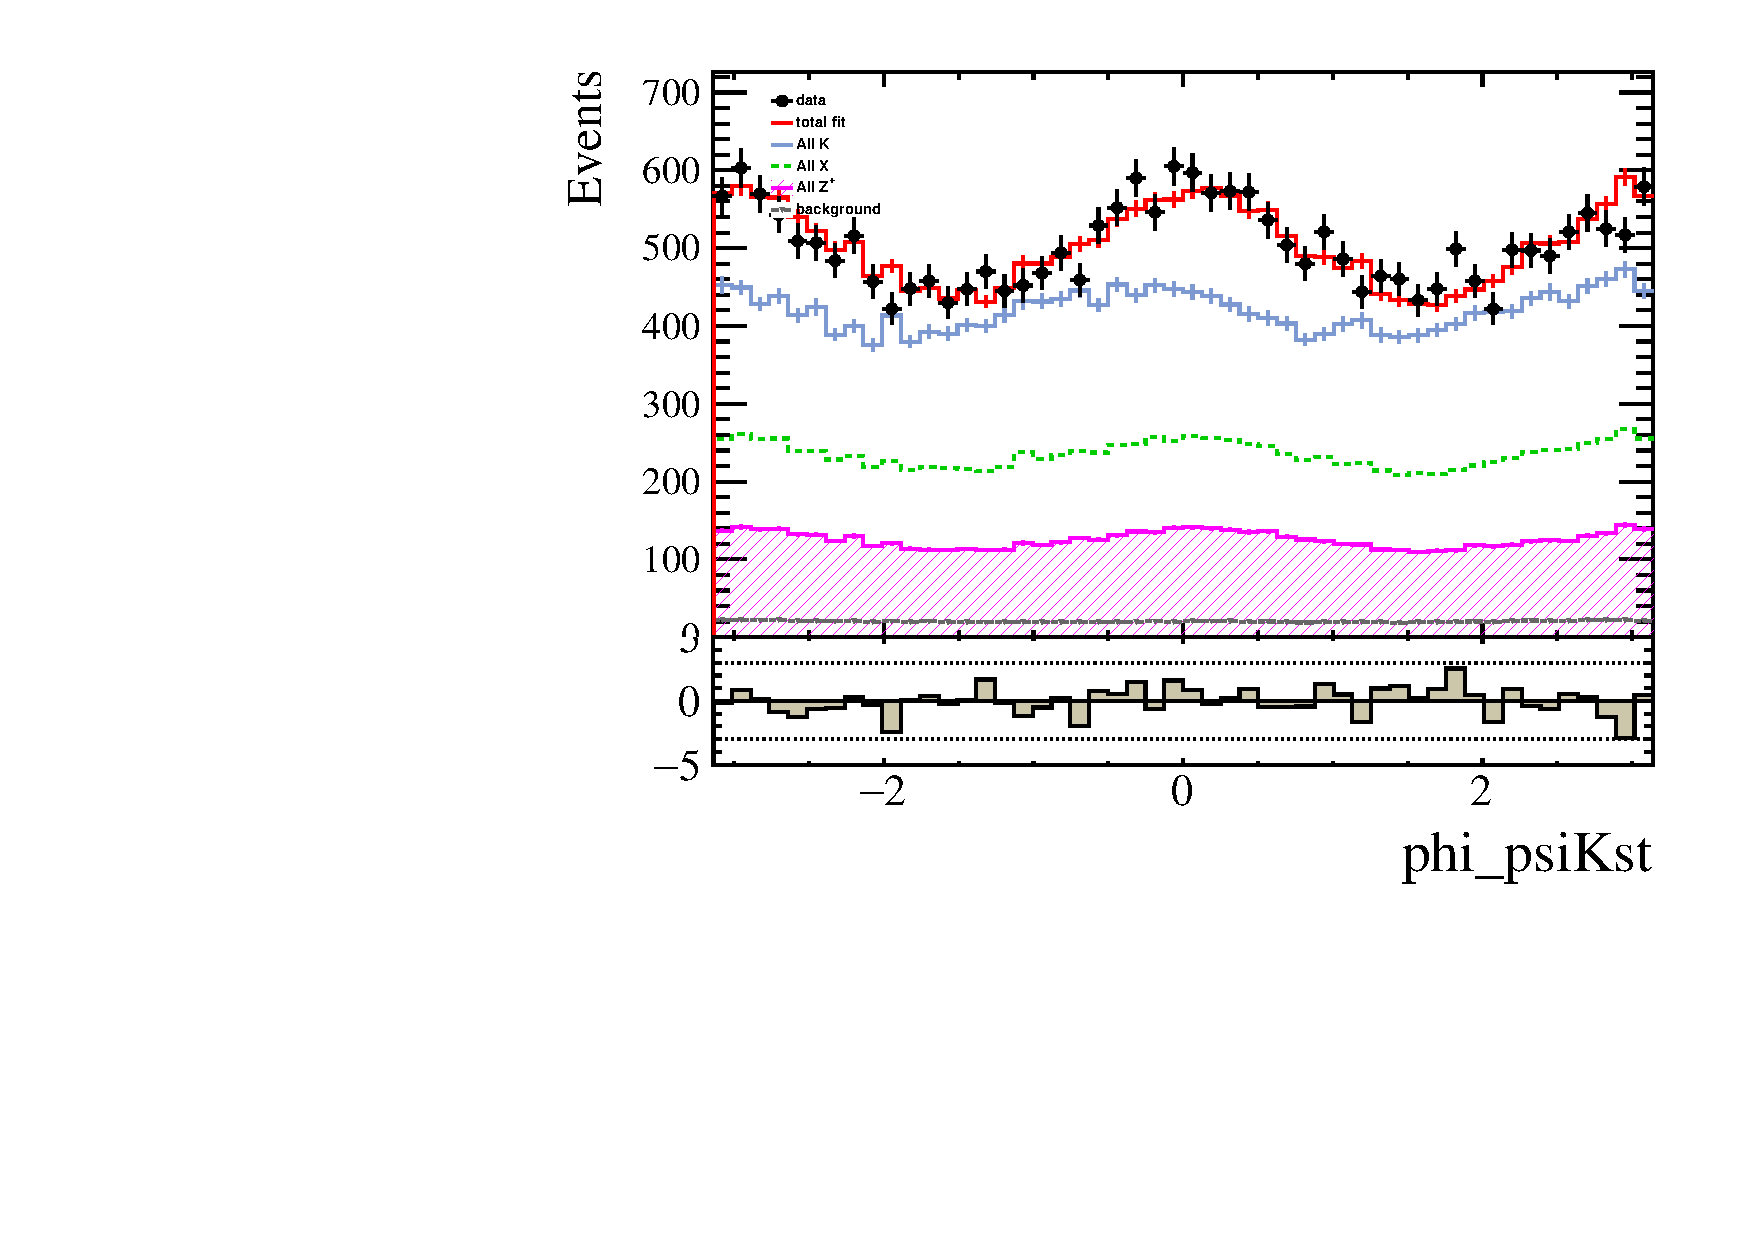
\includegraphics[width=0.5\textwidth]{Figures/03_Zcs/06_Amplitude/fitx2m/phi_psiKst}
\put(-80,145) {\textrm{\small \bf(b) $\phikspsi$}}
\\
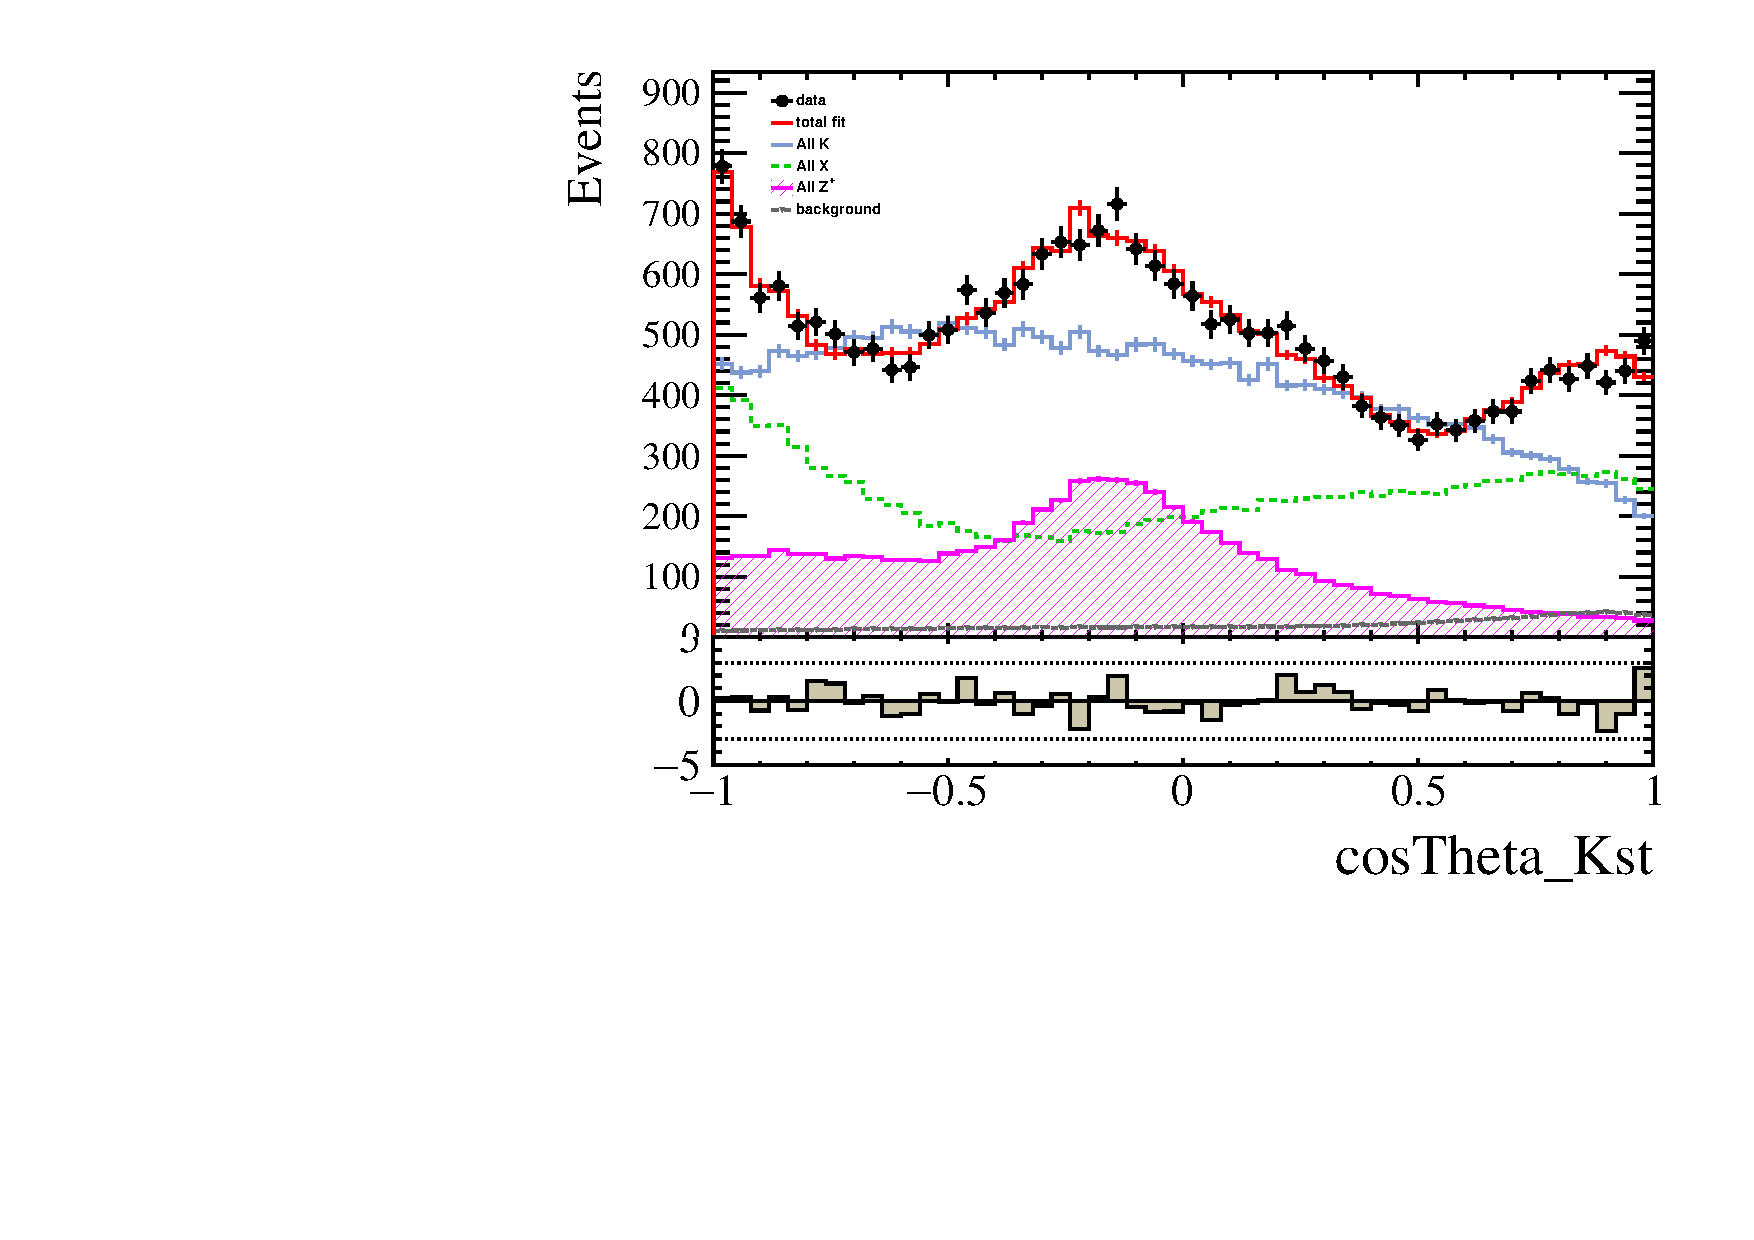
\includegraphics[width=0.5\textwidth]{Figures/03_Zcs/06_Amplitude/fitx2m/cosTheta_Kst}%
\put(-80,145) {\textrm{\small \bf(c) $\cosks$}}
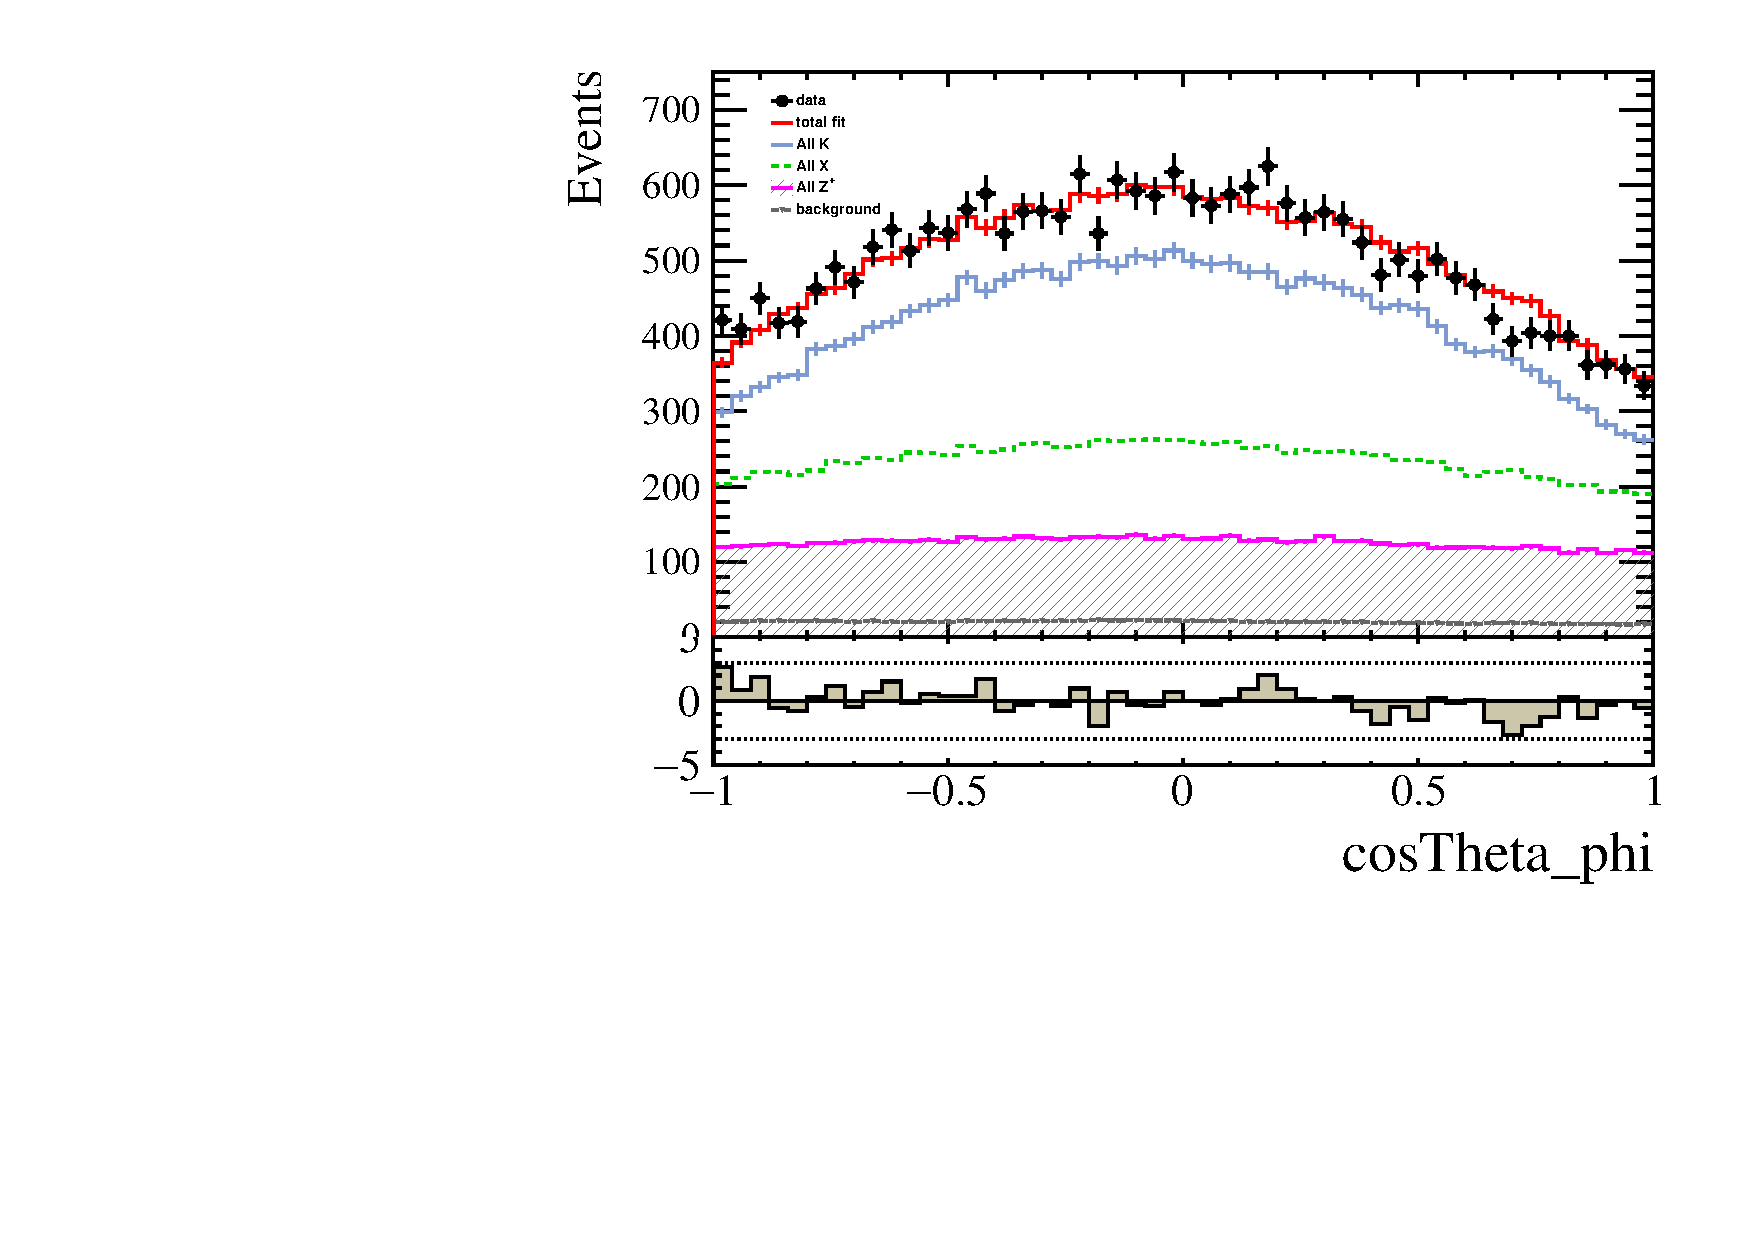
\includegraphics[width=0.5\textwidth]{Figures/03_Zcs/06_Amplitude/fitx2m/cosTheta_phi}
\put(-80,145) {\textrm{\small \bf(d) $\cosphi$}}\\
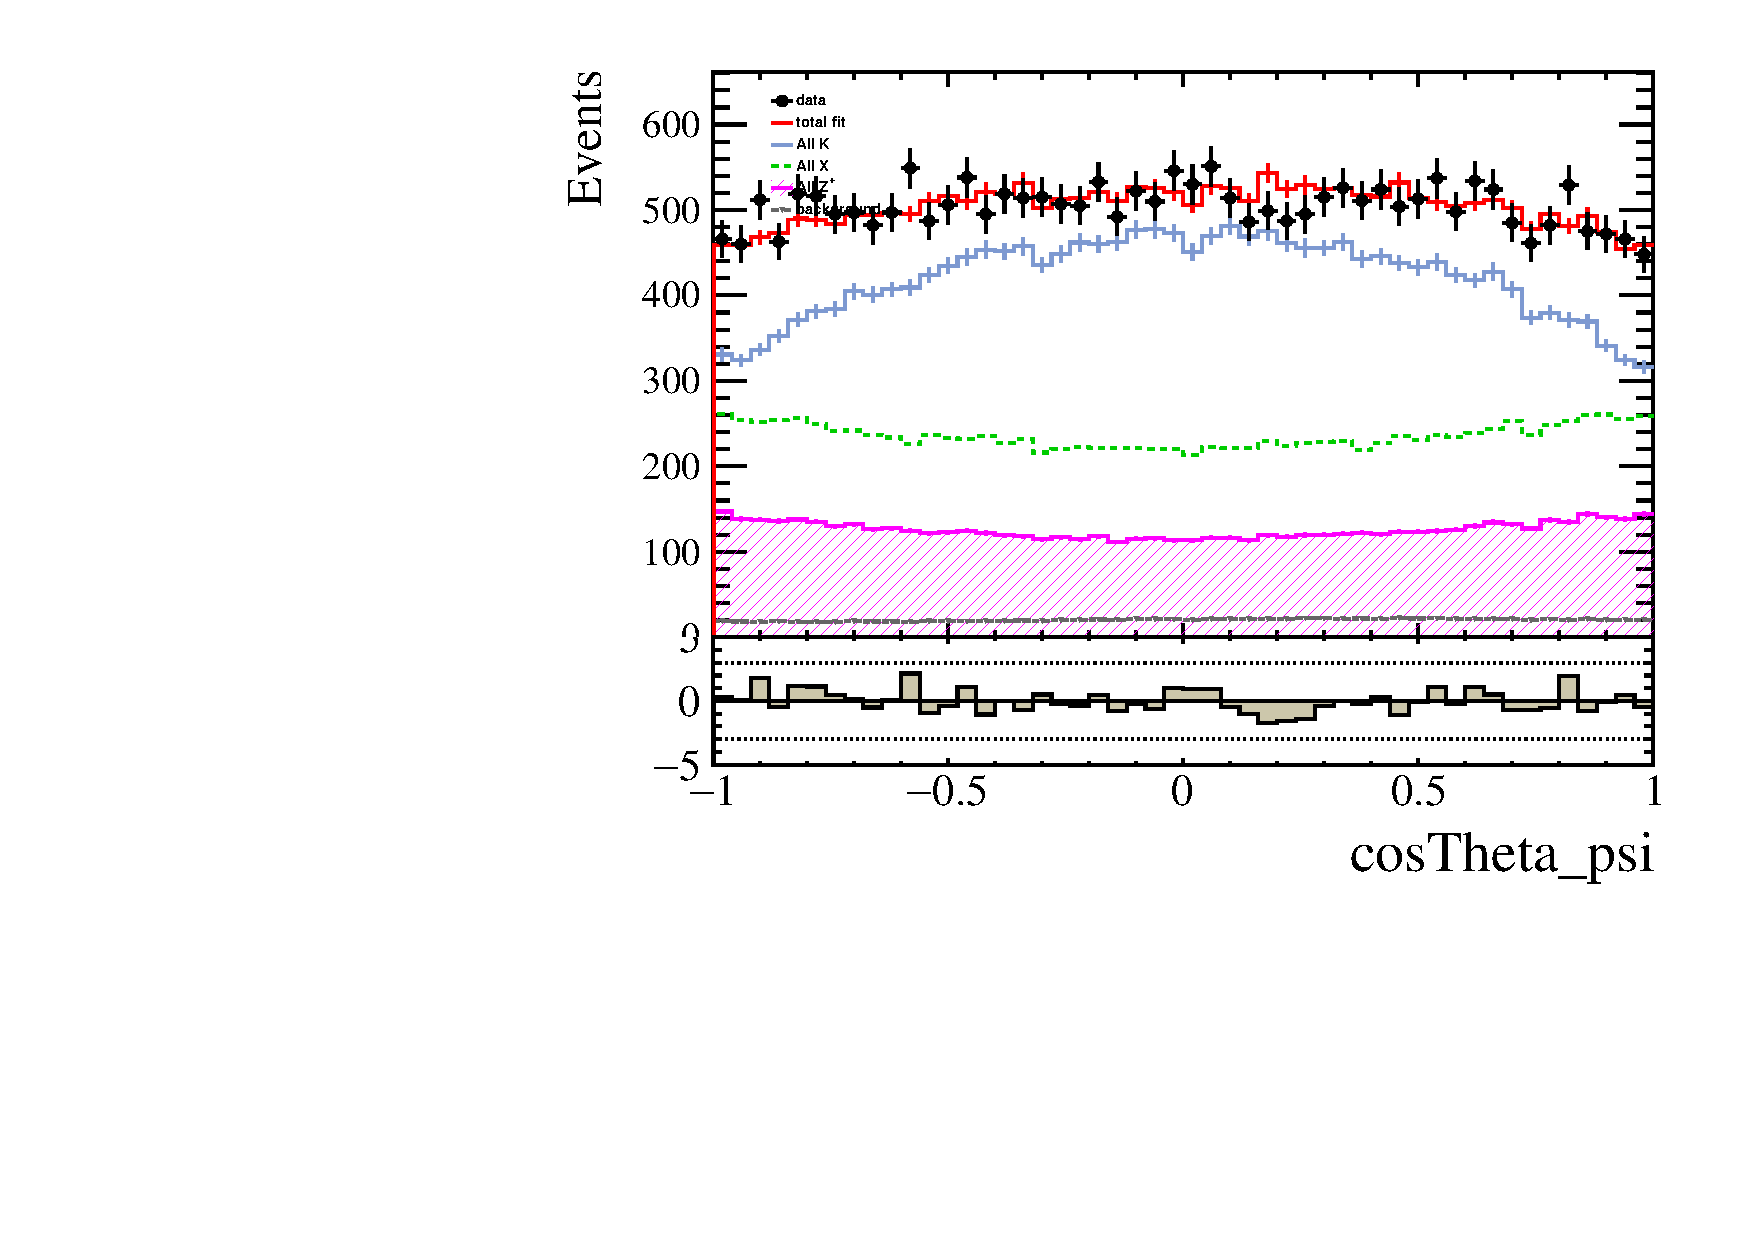
\includegraphics[width=0.5\textwidth]{Figures/03_Zcs/06_Amplitude/fitx2m/cosTheta_psi}
\put(-80,145) {\textrm{\small \bf(e) $\cospsi$}}\\
\caption{Fit projections of angles in the $\phi K$ decay chain.}
\label{fig:ang}
\end{figure}




\begin{table}[tbph]
\begin{center}
\caption{Fit results from  the 9K+5X+3X+2Z model with $Z_{cs}(4220)$ $J^P=1^+$. 
Significance is evaluated from the change of the $2\ln\Like$ assuming ndf to be {\bf twice} the reduction in number of free parameters when removing the component in the fit. 
The ndf is not multiply by two for the $K^*$ resonance whose mass and width are fixed.}\label{tab:fit}
\begin{tabular}{cccccc}
\hline
\multicolumn{2}{c}{Contribution} &Significance & \multicolumn{3}{c}{Fit results}  \\
                  &                           &                 & $M_0$ [MeV]   & $\Gamma_0$ [MeV]      & FF\%          \\
\hline \hline
   &     All $K(1^+)$    &        &    &   &  $25.1\pm3.6$          \\
$\nslj{2}{1}{P}{1}$   &  $K(1^+)$             & 4.5$\sigma$  &  $1861\pm 10 $  &  $149\pm41$  &       \\
$\nslj{2}{3}{P}{1}$   &  $K^{\prime}$($1^+$)  & 4.5$\sigma$  &  $1911\pm 37 $  &  $276\pm50$  &       \\
$\nslj{1}{3}{P}{1}$   &  $K_1(1400)$          & 11$\sigma$  &  &     &   $15.1\pm2.7$    \\
\hline

&     All $K(2^-)$    &        &        & &  $2.1\pm0.4$           \\
$\nslj{1}{1}{D}{2}$   &  $K_2 (1770)$   & 8.0$\sigma$       &    &    &     \\
$\nslj{1}{3}{D}{2}$   &  $K_2(1820)$    & 5.8$\sigma$       &    &    &     \\       

\hline
& All $K(1^-)$        & & & & $50.3\pm4.1$ \\
$\nslj{1}{3}{D}{1}$   &  $K^*(1680)$    & 13$\sigma$  &   &    &  $13.5\pm2.3$    \\  
$\nslj{2}{3}{S}{1}$   &  $K^*(1410)$    & 15$\sigma$   &   &    &  $37.9\pm5.2$   \\
\hline

& $K(2^+)$\\
$\nslj{2}{3}{P}{2}$   &  $K^*_2(1980)$  & 7.4$\sigma$   &  $1988\pm22 $   &   $318\pm82$   & $2.3\pm0.5$        \\  
\hline 
& $K(0^-)$\\
$\nslj{2}{1}{S}{0}$   &  $K(1460)$      & 13$\sigma$       &    &      & $10.2\pm1.2$    \\  

\hline 
\hline
&$X(2^-)$ & & & &   \\
  &$X(4150)$            & $8.7\sigma$ & $4146\pm 18$ & $135\pm28$   & $2.0\pm0.5$ \\
\hline
&$X(1^-)$ & & & &   \\
  &$X(4630)$            & $5.7\sigma$ & $4626\pm 16$ & $174\pm27$  & $2.6\pm0.5$ \\
\hline

 &All $X(0^+)$ & & & & $19.5\pm4.8$  \\
 &$X(4500)$           & $20\sigma$ & $4474\pm 3$ & $77\pm6$ &  $5.6\pm0.7$ \\
 &$X(4700)$           & $18\sigma$ & $4694\pm 4$ & $87\pm8$ &  $8.9\pm1.2$ \\
 &$NR_{J/\psi \phi}$  & $5.7 \sigma $& & &$28.0\pm7.5$ \\
\hline
 &All $X(1^+)$ & & & & $26.0\pm3.4$ \\
 &$X(4140)$           & $16\sigma$ & $4118\pm 11$ & $162\pm21$ & $17.2\pm2.9$ \\
 &$X(4274)$           & $18\sigma$ & $4294\pm 4$  & $53\pm5$   & $2.8\pm0.49$ \\
 &$X(4685)$           & $15\sigma$ & $4684\pm 7$  & $126\pm15$ & $7.2\pm1.0$ \\
\hline\hline
&All $Z(1^+)$ & & & & $25.0\pm4.9$ \\
  &$Z_{cs}(4000)$          & $16\sigma$ & $4003\pm 6$  & $131\pm15$  & $9.4\pm2.1$ \\
  &$Z_{cs}(4220)$          & $8.4\sigma$ & $4216\pm 24$ & $233\pm52$ & $10.3\pm3.8$ \\
\hline
\end{tabular}
\end{center}
\end{table}



\subsection{Extended $K^*$ model}
We add more $K^*$ resonances to test the significance of each of components, 
and evaluate systematic uncertainties. 
Seven more $K$ resonances are predicted in the allowed $\phi K$ mass range by the relativistic potential model from Godfrey-Isgur~\supercite{Godfrey:1985xj}. 
They are $\nslj{3}{1}{S}{0}(0^-)$, $\nslj{3}{3}{S}{1}(1^-)$, $\nslj{1}{3}{D}{3}(3^-)$,$1^{1,3}\mathrm{F}_3(3^+)$, $\nslj{1}{3}{F}{2}(2^+)$, and $\nslj{1}{3}{F}{4}(4^+)$. 
%Adding each of them individually doesn't improve the fit by more than $3\,\sigma$ significance. <=== Seems to be contradicted by the results in the table below, even if true, better not to confuse people
We add all of them except for the $4^+$ resonance because $L_{B}=3$ decays of $B$ are expected to be much suppressed. 
We use only one BW to represent $1^{1,3}\mathrm{F}_3(3^+)$ resonances to reduce possible large interference effects between these two states predicted to be very close in mass. 
The fit results are listed in Table~\ref{tab:fitextend}. 
All the new exotic components preserve large significances of more than $5\sigma$.  
Among additional $K^*$ components, 
a candidate $\nslj{3}{3}{S}{1}$ state is $4.4\sigma$ significant, 
and has large mass and width, 
as expected for such high radial excitation of triplet $S-$wave. 
A candidate for higher radial excitation of the singlet $S-$wave $\nslj{3}{1}{S}{0}$ has a significance of $4.6\sigma$, 
but very small fit fraction.
Other states are even less significant. 
The mass projections of this fit are shown in Figure.~\ref{fig:fitext}.
%The data and the model are also compared on the angular moments as discussed in Appendix~\ref{sec:app:Y}. Appendix only compared run-1 and nominal model fits.

\begin{figure}[!tbp]
\centering
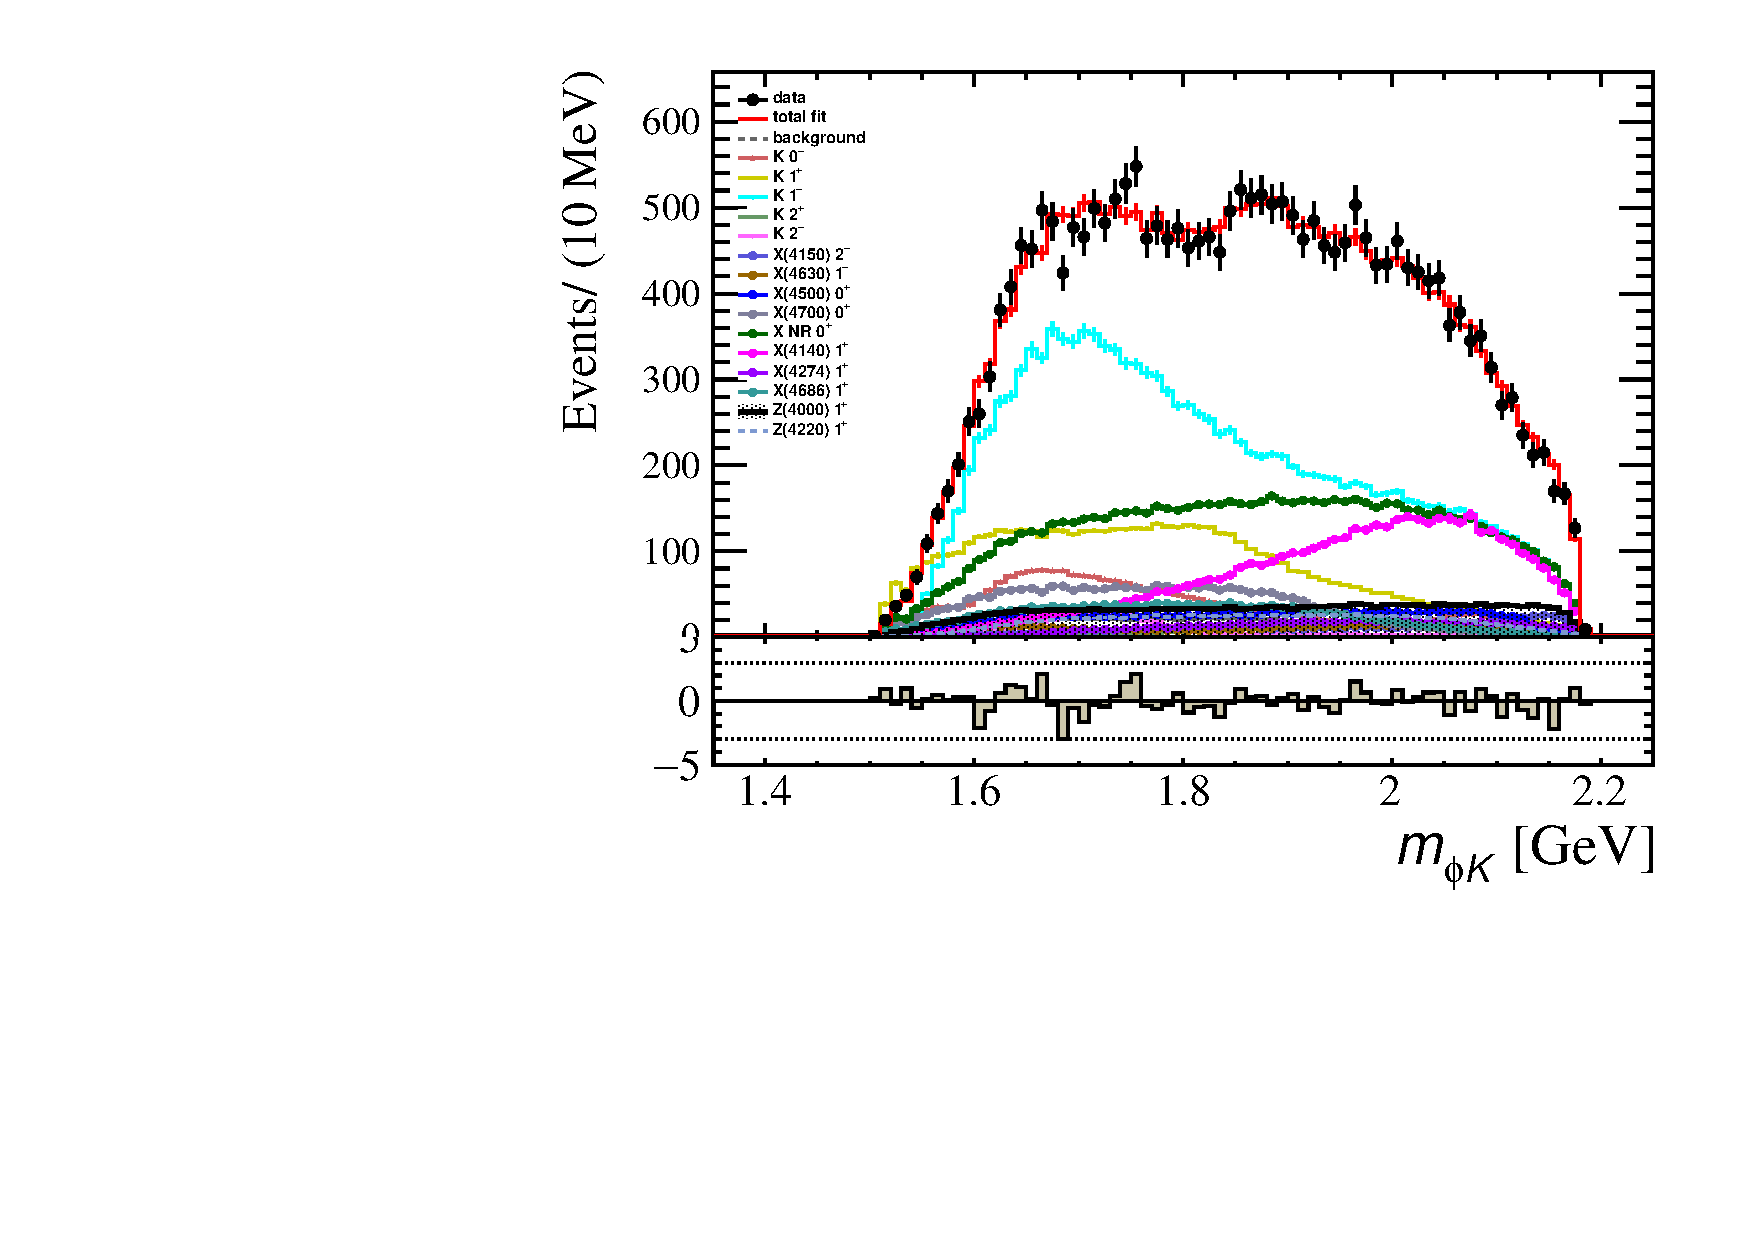
\includegraphics[width=0.6\textwidth]{Figures/03_Zcs/06_Amplitude/fitallk/mphik-AllKZ1P}
\put(-60,168) {\textrm{\small \bf(a)}}\\
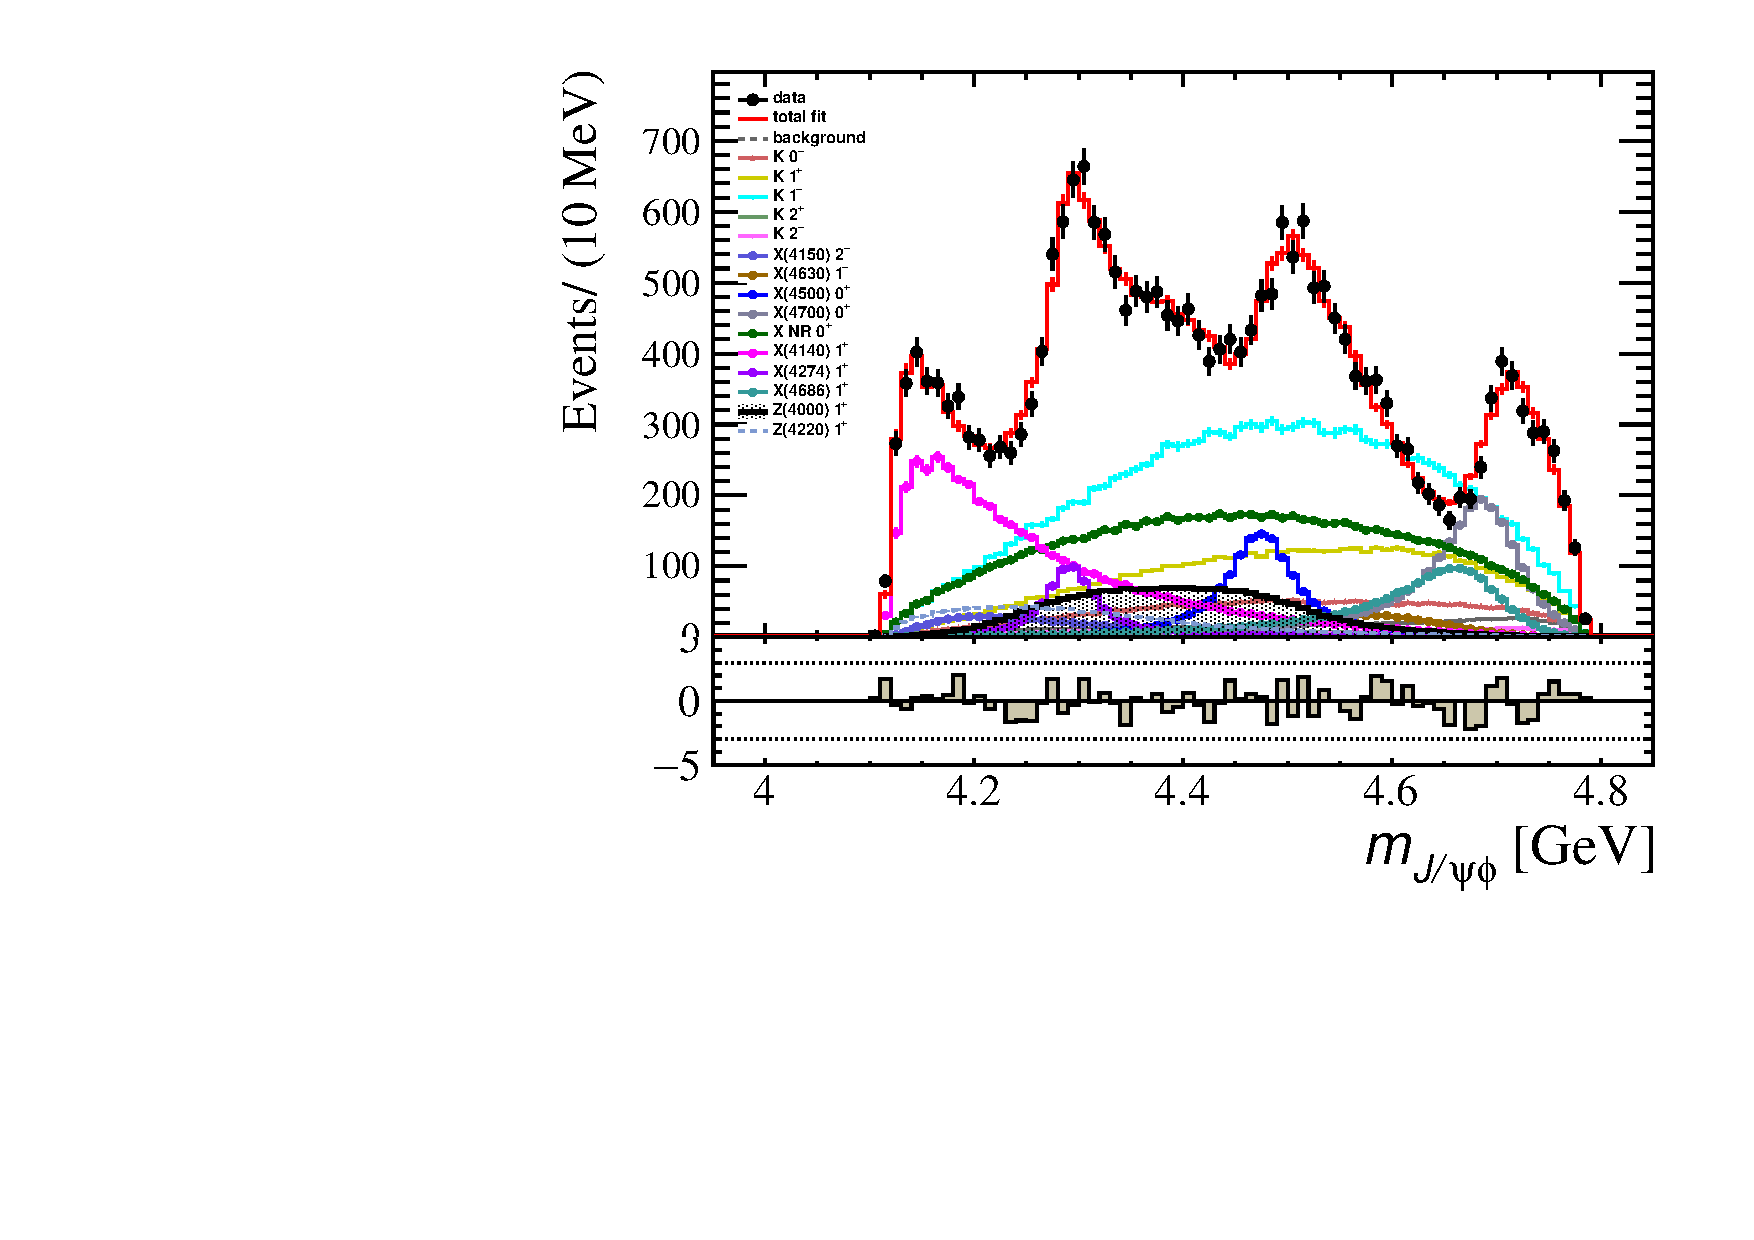
\includegraphics[width=0.6\textwidth]{Figures/03_Zcs/06_Amplitude/fitallk/mjpsiphi-AllKZ1P}
\put(-60,168) {\textrm{\small \bf(b)}}\\
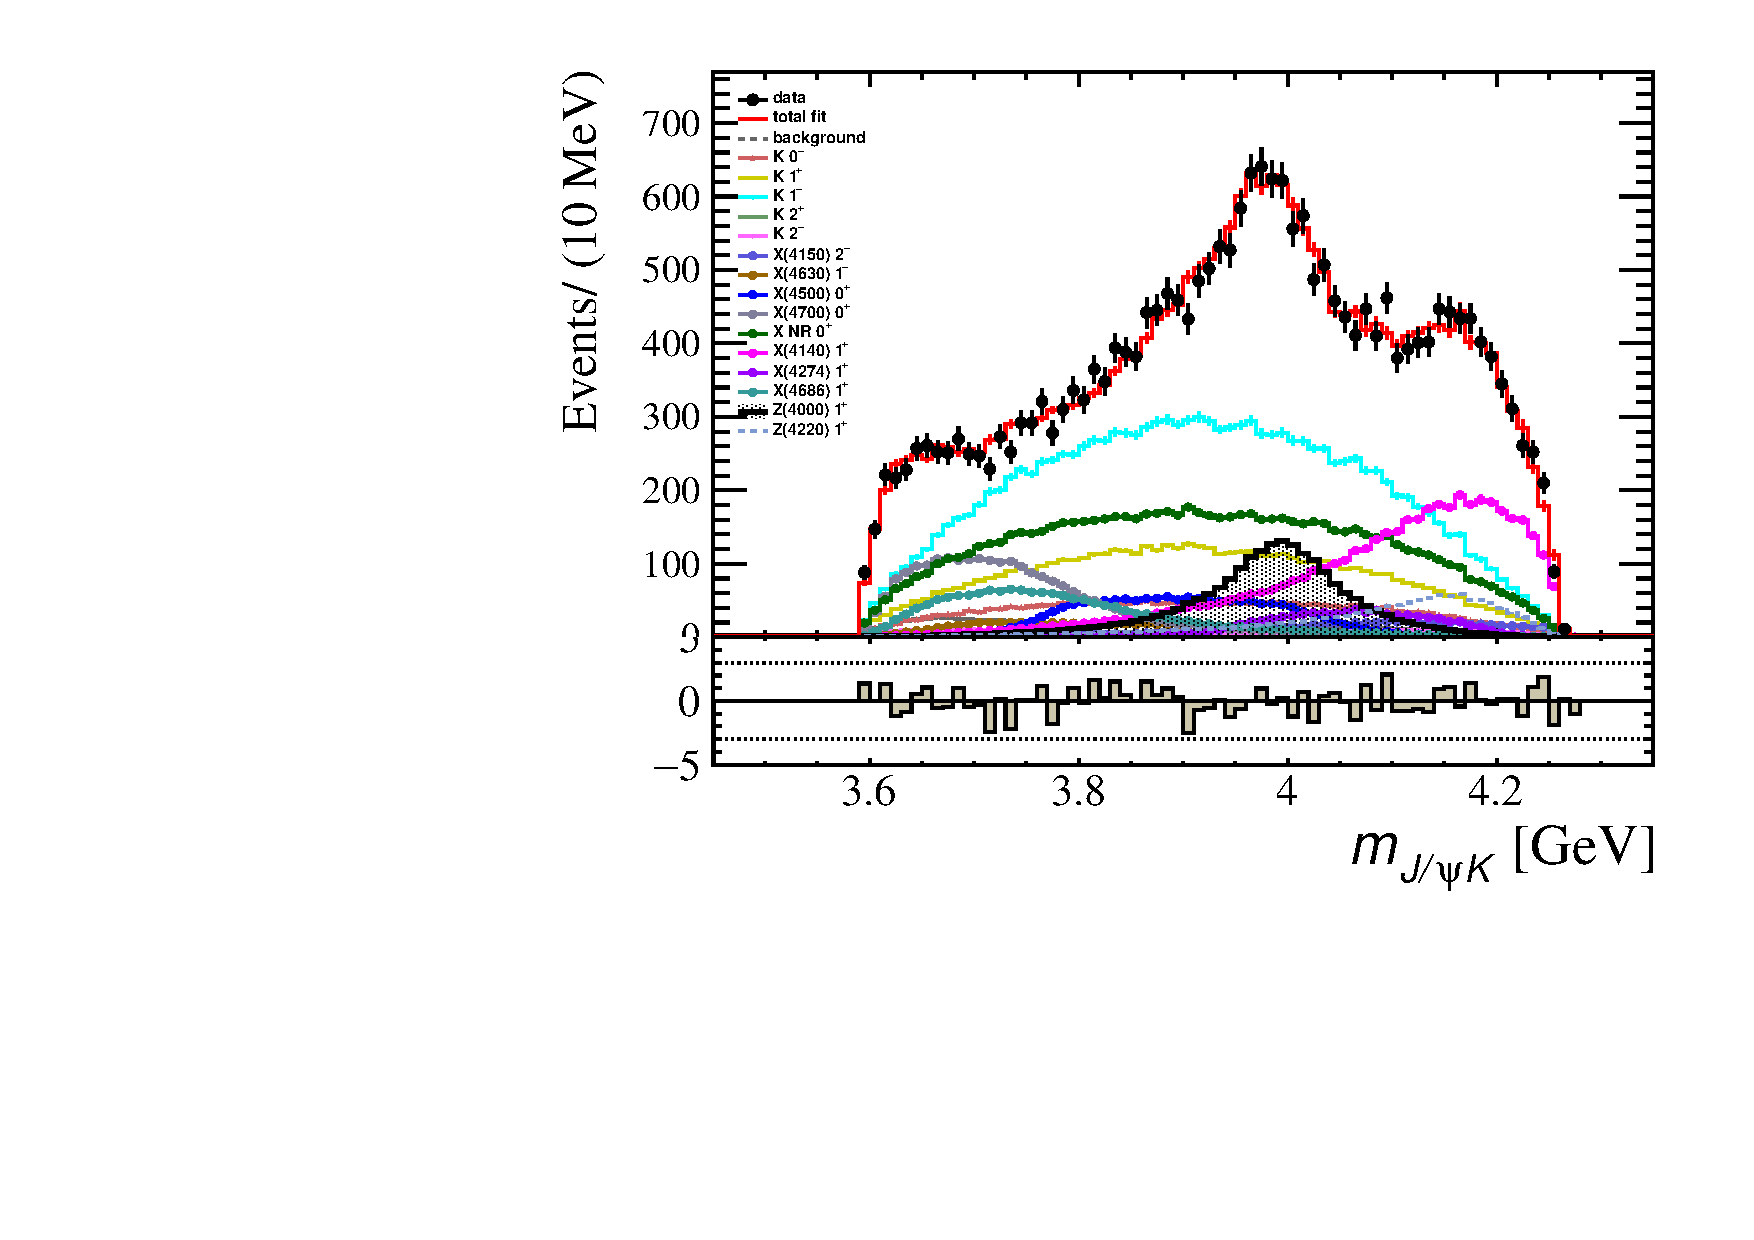
\includegraphics[width=0.6\textwidth]{Figures/03_Zcs/06_Amplitude/fitallk/mjpsik-AllKZ1P}
\put(-60,168) {\textrm{\small \bf(c)}}
\caption{Fit projections of (a) $\mfk$, (b) $\mjf$, (c) $\mjk$ from the Extended K+5X+2X+2Z model.}
\label{fig:fitext}
\end{figure}

\begin{table}[tbph]
\begin{center}
\caption{Fit results from  Extended K+5X+3X+2Z model for $X(4220)$ with $J^P=1^+$. 
Significance is evaluated from the change of the $2\ln\Like$ assuming ndf to be {\bf twice} the reduction in number of free parameters when removing the component in the fit. 
The factor of two is not applied when mass and width are fixed. 
The two F $K$ states have almost zero fit fractions and significances, 
therefore, their masses and widths from the fit are meaningless and not shown. }\label{tab:fitextend}
\begin{tabular}{cccccc}
\hline
\multicolumn{2}{c}{Contribution} &Significance & \multicolumn{3}{c}{Fit results}  \\
                  &                           &                 & $M_0$ [MeV]   & $\Gamma_0$ [MeV]      & FF\%          \\
\hline \hline
  & All $K(1^+)$    &        &    &   &  $23.2$          \\
$\nslj{2}{1}{P}{1}$   &   $K(1^+)$              & 4.9$\sigma$     &  $1821\pm 15 $   &  $372\pm 63$   &        \\
$\nslj{2}{3}{P}{1}$   &   $K^{\prime}$($1^+$)   & 4.9$\sigma$    &  $1871\pm 20 $   &  $154\pm 28$   &     \\
$\nslj{1}{3}{P}{1}$   &   $K_1(1400)$           & 9.2$\sigma$     &   &   &   15.0   \\
\hline
   &     All $K(2^-)$   &        &      & &  $2.1$           \\
$\nslj{1}{1}{D}{2}$   &  $K_2 (1770)$  & 7.9$\sigma$       &    &     &      \\
$\nslj{1}{3}{D}{2}$   &  $K_2(1820)$   & 6.4$\sigma$        &    &     &        \\       

\hline
& All $K(1^-)$ & & & & $52.5$ \\
$\nslj{1}{3}{D}{1}$   & $K^*(1680)$  & 4.7$\sigma$  &    &                           & $6.4$     \\  
$\nslj{2}{3}{S}{1}$   & $K^*(1410)$  & 7.7$\sigma$   &    &                           & $34.2$ \\
$\nslj{3}{3}{S}{1}$   &              & 4.4$\sigma$  & $2128\pm36 $   &   $448\pm132$  & $4.5$ \\
\hline

& All $K(2^+)$ &  & & & $1.6$\\
$\nslj{2}{3}{P}{2}$  &  $K^*_2(1980)$  & 1.6$\sigma$    & $2182\pm73$ & $800\pm230$    & $2.4$ \\
$\nslj{1}{3}{F}{2}$  &       &      1.3$\sigma$  &   $2076\pm25$ & $100\pm74$        & $0.4$  \\
\hline 
& All $K(0^-)$& & & & $10.0$\\
$\nslj{2}{1}{S}{0}$  &  $K(1460)$    & 12$\sigma$      &    &                        & $11.0$    \\  
$\nslj{3}{1}{S}{0}$  &               & 4.6$\sigma$      &$2064\pm15$  & $108\pm46$ & $0.5$ \\
\hline 
$\nslj{1}{1}{F}{3}$  &  $K(3^+)$     &0.3$\sigma$       &   &    & 0.2 \\
\hline 
$\nslj{1}{3}{D}{3}$  &  $K(3^-)$     &2.3$\sigma$       &  &   & 0.2 \\

\hline 
\hline
&$X(2^-)$ & & & &   \\
  &$X(4150)$ & $6.3\sigma$ & $4117\pm 13$ & $193\pm81$ & $2.8$ \\
\hline
&$X(1^-)$ & & & &   \\
  &$X(4630)$ & $5.5\sigma$ & $4611\pm 28$ & $193\pm25$ & $2.7$ \\
\hline

 &All $X(0^+)$ & & & & $22.8$  \\
 &$X(4500)$ & $20\sigma$ & $4476\pm 3$ & $73\pm6$ &  $5.6$ \\
 &$X(4700)$ & $17\sigma$ & $4695\pm 4$ & $89\pm9$ & $9.2$ \\
 &$NR_{J/\psi \phi}$ & $4.8 \sigma $& & &$33.0$ \\
\hline
 &All $X(1^+)$ & & & & $31.2$ \\
 &$X(4140)$ & $13\sigma$ & $4107\pm 12$ & $138\pm22$ & $21.1$ \\
 &$X(4274)$ & $18\sigma$ & $4293\pm 3$ & $53\pm5$   & $3.1$ \\
 &$X(4685)$ & $15\sigma$ & $4681\pm 9$ & $120\pm17$ & $6.3$ \\
\hline\hline
&All $Z(1^+)$ & & & & $15.9$ \\
  &$Z_{cs}(4000)$ & $15\sigma$ & $4001\pm 5$ & $124\pm19$ & $8.2$ \\
  &$Z_{cs}(4220)$ & $5.9\sigma$ & $4196\pm 22$ & $176\pm35$ & $5.6$ \\
\hline
\end{tabular}
\end{center}
\end{table}


\iffalse
\begin{table}[tbph]
\begin{center}
\caption{Fit results from  Extended K+5X+3X+2Z model. 
Significance is evaluated from the change of the $2\ln\Like$ assuming ndf to be {\bf twice} the reduction in number of free parameters when removing the component in the fit. 
The factor of two is not applied when mass and width are fixed. 
The two F $K$ states have almost zero fit fractions and significances,  
their meaningless fit masses and widths are not shown. }\label{tab:fitextend}
\begin{tabular}{cccccc}
\hline
\multicolumn{2}{c}{Contribution} &Significance & \multicolumn{3}{c}{Fit results}  \\
                  &                           &                 & $M_0$ [MeV]   & $\Gamma_0$ [MeV]      & FF\%          \\
\hline \hline
  & All $K(1^+)$    &        &    &   &  $20.7$          \\
$\nslj{2}{1}{P}{1}$   &   $K(1^+)$              & 6.4$\sigma$     &  $1838\pm 13 $   &  $398\pm 57$   &        \\
$\nslj{2}{3}{P}{1}$   &   $K^{\prime}$($1^+$)   & 6.4$\sigma$    &  $1888\pm 14 $   &  $107\pm 23$   &     \\
$\nslj{1}{3}{P}{1}$   &   $K_1(1400)$           & 6.8$\sigma$     &   &   &   13.8   \\
\hline
   &     All $K(2^-)$   &        &      & &  $3.6$           \\
$\nslj{1}{1}{D}{2}$   &  $K_2 (1770)$  & 10$\sigma$       &    &     &      \\
$\nslj{1}{3}{D}{2}$   &  $K_2(1820)$   & 8.5$\sigma$        &    &     &        \\       

\hline
& All $K(1^-)$ & & & & $85.8$ \\
$\nslj{1}{3}{D}{1}$   & $K^*(1680)$  & 7.8$\sigma$  &    &                           & $5.7$     \\  
$\nslj{2}{3}{S}{1}$   & $K^*(1410)$  & 9.6$\sigma$   &    &                           & $32.4$ \\
$\nslj{3}{3}{S}{1}$   &              & 6.2$\sigma$  & $2182_{-12}^{+100} $   &   $650\pm159$  & $21.7$ \\
\hline

& All $K(2^+)$ &  & & & $1.6$\\
$\nslj{2}{3}{P}{2}$  &  $K^*_2(1980)$  & 1.6$\sigma$    & $2043\pm73$ & $419\pm127$    & $2.8$ \\
$\nslj{1}{3}{F}{2}$  &       &      0.4$\sigma$  &   &        & $0.3$  \\
\hline 
& All $K(0^-)$& & & & $8.7$\\
$\nslj{2}{1}{S}{0}$  &  $K(1460)$    & 14$\sigma$      &    &                        & $9.4$    \\  
$\nslj{3}{1}{S}{0}$  &               & 4.2$\sigma$      &$2071\pm15$  & $88\pm30$ & $0.3$ \\
\hline 
$\nslj{1}{1}{F}{3}$  &  $K(3^+)$     &0.2$\sigma$       &   &    & 0.1 \\
\hline 
$\nslj{1}{3}{D}{3}$  &  $K(3^-)$     &0.7$\sigma$       &  &   & 0.1 \\

\hline 
\hline
&$X(2^-)$ & & & &   \\
  &$X(4175)$ & $5.3\sigma$ & $4117\pm 13$ & $194\pm58$ & $4.5\pm0.5$ \\
\hline
&$X(1^-)$ & & & &   \\
  &$X(4650)$ & $9.4\sigma$ & $4632\pm 25$ & $340\pm72$ & $4.8\pm0.5$ \\
\hline

 &All $X(0^+)$ & & & & $19.0\pm4.8$  \\
 &$X(4500)$ & $18\sigma$ & $4477\pm 3$ & $66\pm5$ &  $4.8\pm0.7$ \\
 &$X(4700)$ & $18\sigma$ & $4690\pm 4$ & $86\pm9$ & $8.4\pm1.2$ \\
 &$NR_{J/\psi \phi}$ & $8.4 \sigma $& & &$24.0\pm7.6$ \\
\hline
 &All $X(1^+)$ & & & & $54.7\pm3.4$ \\
 &$X(4140)$ & $15\sigma$ & $4107\pm 12$ & $168\pm21$ & $43.2\pm2.9$ \\
 &$X(4274)$ & $19\sigma$ & $4298\pm 4$ & $57\pm6$   & $3.4\pm0.4$ \\
 &$X(4675)$ & $16\sigma$ & $4683\pm 8$ & $127\pm17$ & $7.\pm1.12$ \\
\hline\hline
&$Z(1^+)$ \\
  &$Z_{cs}(3990)$ & $17\sigma$ & $3991\pm 4$ & $102\pm12$ & $5.5$ \\
  \hline
&$Z(1^-)$ \\
  &$Z_{cs}(4260)$ & $6.7\sigma$ & $4219\pm 27$ & $289\pm68$ & $4.5$ \\
\hline
\end{tabular}
\end{center}
\end{table}
\fi


In all the models, 
the two new $X$ states around 4650\mev are found to have significance of more than $5\sigma$, each. 
Together with the $X(4700)$ state, 
there are three $X$ states around this mass region. 
We use $\chisq$ test on $m^2_{\jpsi \phi}$ vs.\  $m^2_{\jpsi K}$ plane to evaluate the fit quality in two-dimensions. 
%The nominal model has $\chisq_{2D}/{\rm nbin}=1027.9/1018$,
%while removing the two new $X$ states gives $1111.7/1018$. 
The nominal model has $\chisq_{2D}/{\rm nbin}=284.5/256$,
while removing the two new $X$ states gives $341.5/256$. 
The contributions to the $\chisq_{2D}$ value for the nominal fit and for the fit without the two $X$ states are compared in Figure.~\ref{fig:chisq2d}. 
The pull distributions are shown in Figure.~\ref{fig:rebin_chisq2d_pull}.

\begin{figure}[!tbp]
\centering
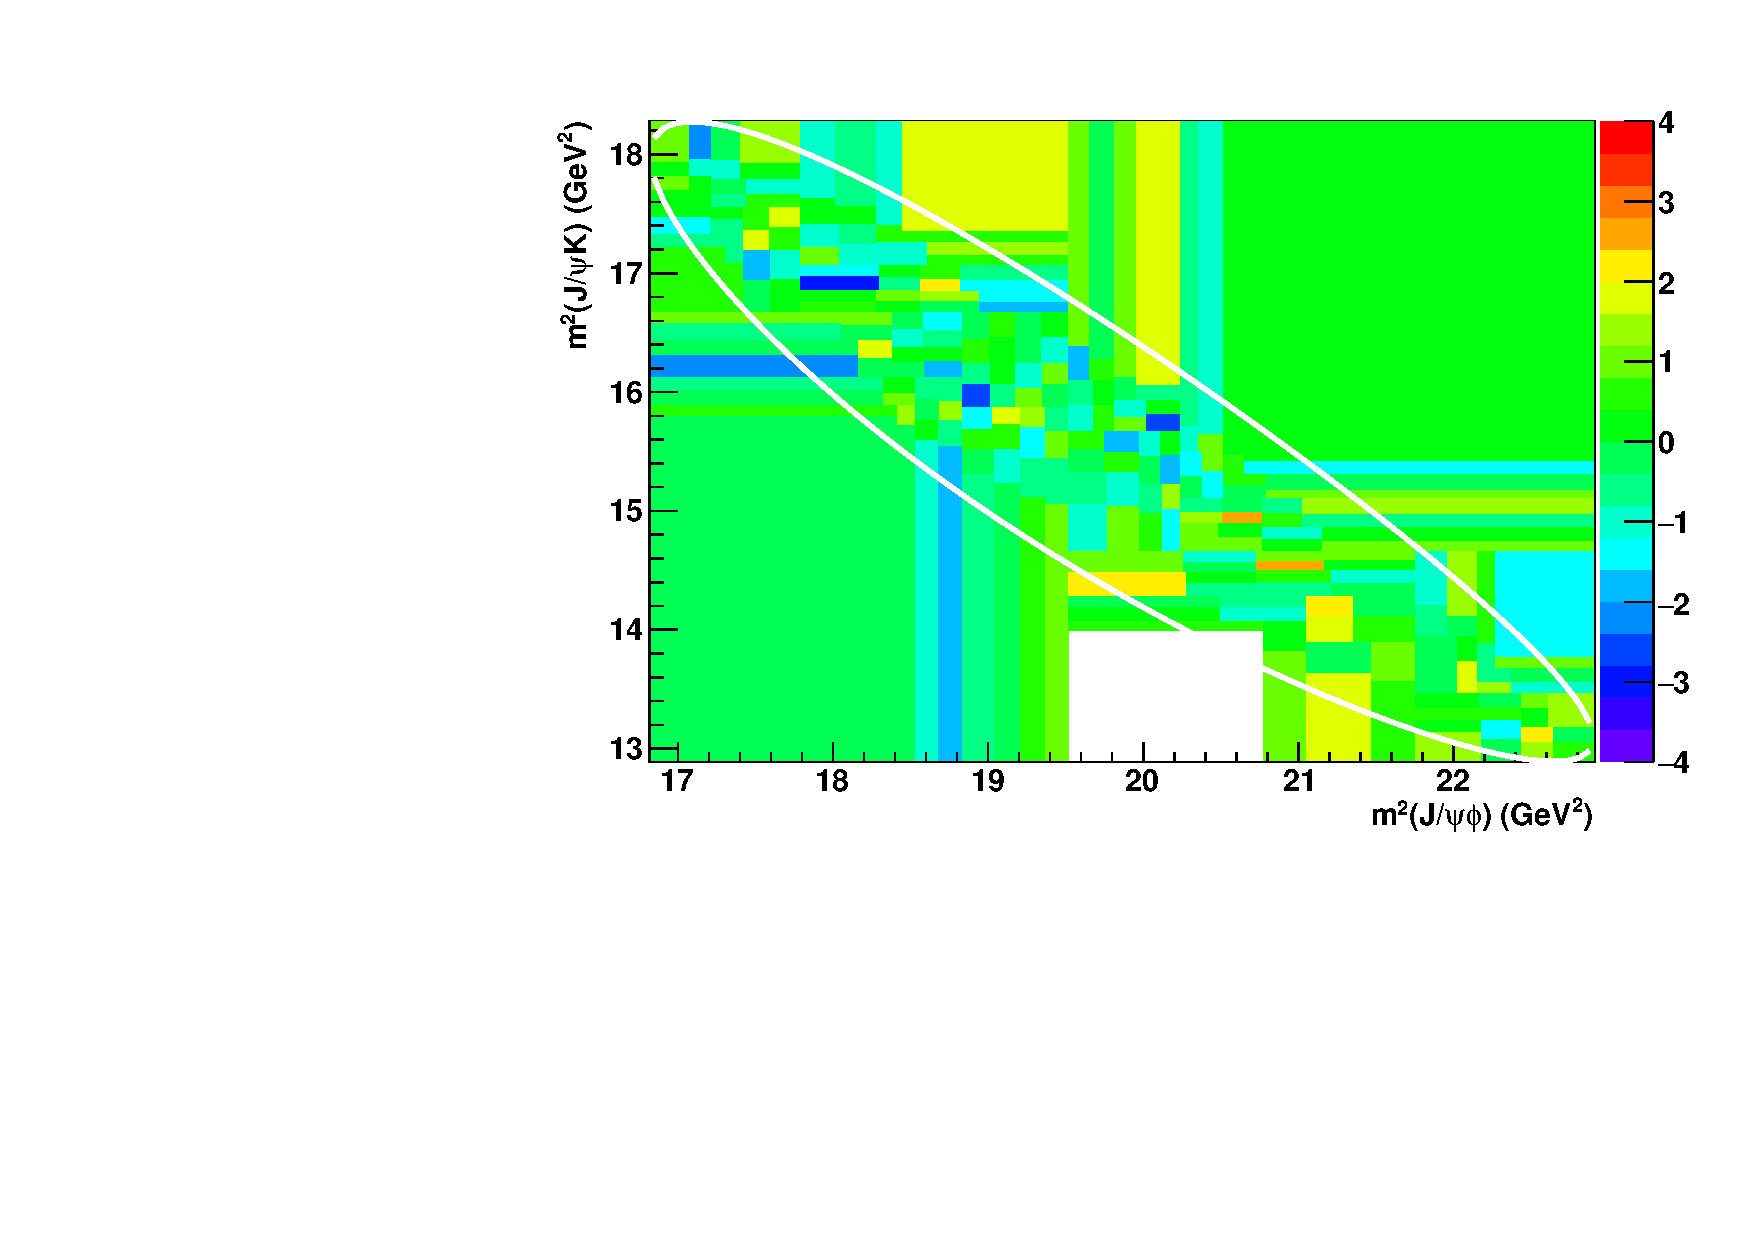
\includegraphics[width=0.7\textwidth]{Figures/03_Zcs/06_Amplitude/noX_plots/resmap_test_norminal.pdf}
\put(-60,168) {\textrm{\small \bf(a)}}\\
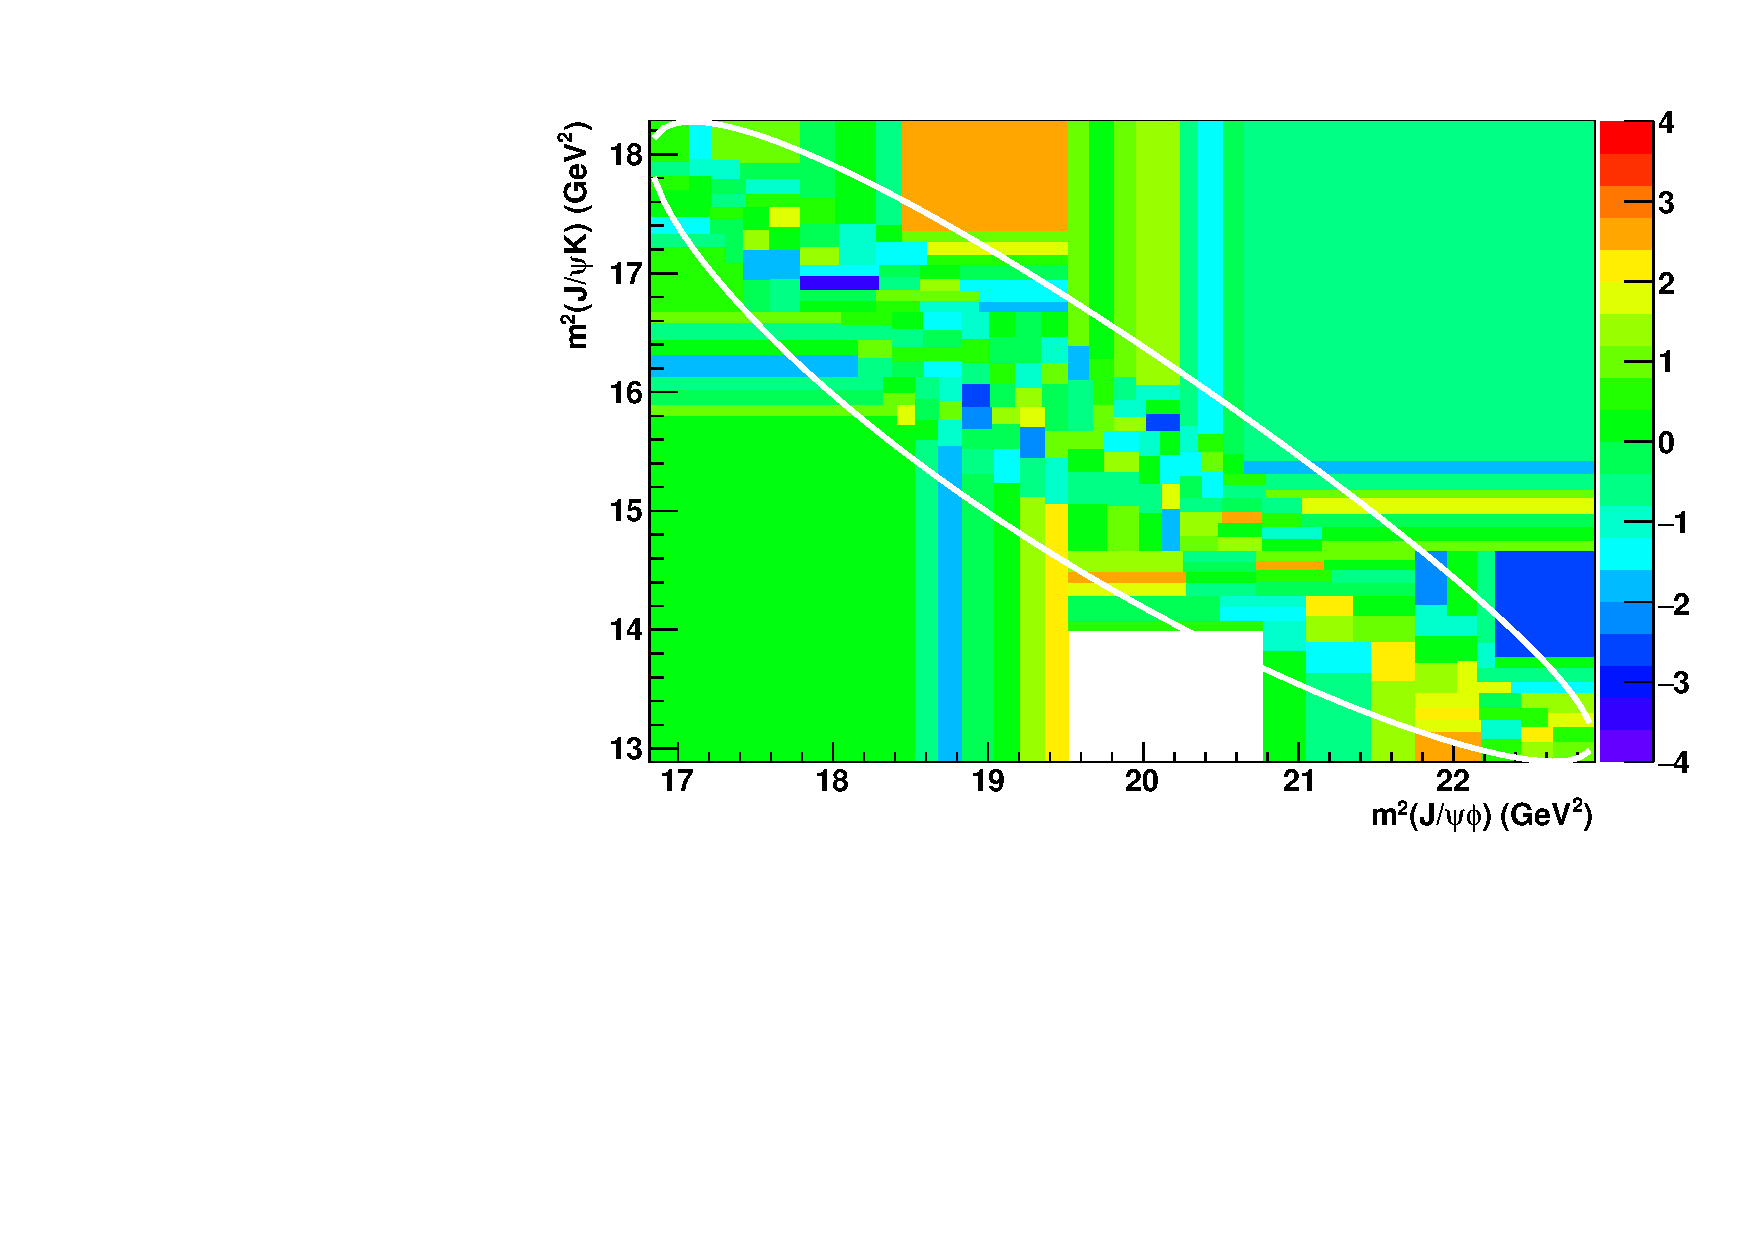
\includegraphics[width=0.7\textwidth]{Figures/03_Zcs/06_Amplitude/noX_plots/resmap_test_noX.pdf}
\put(-60,168) {\textrm{\small \bf(b)}}\\
\caption{Comparison of the standard deviations between the data and the fit model, 
contributing to $\chisq_{2D}$ value, for (a) the nominal fit, and (b) the fit without the two new $X$ states. 
Some improvements are seen in (a) at $m^2(\jpsi\phi)=22$\,GeV$^2$, as compared to (b). }
\label{fig:chisq2d}
\end{figure}

\begin{figure}[!hbtp]
\centering
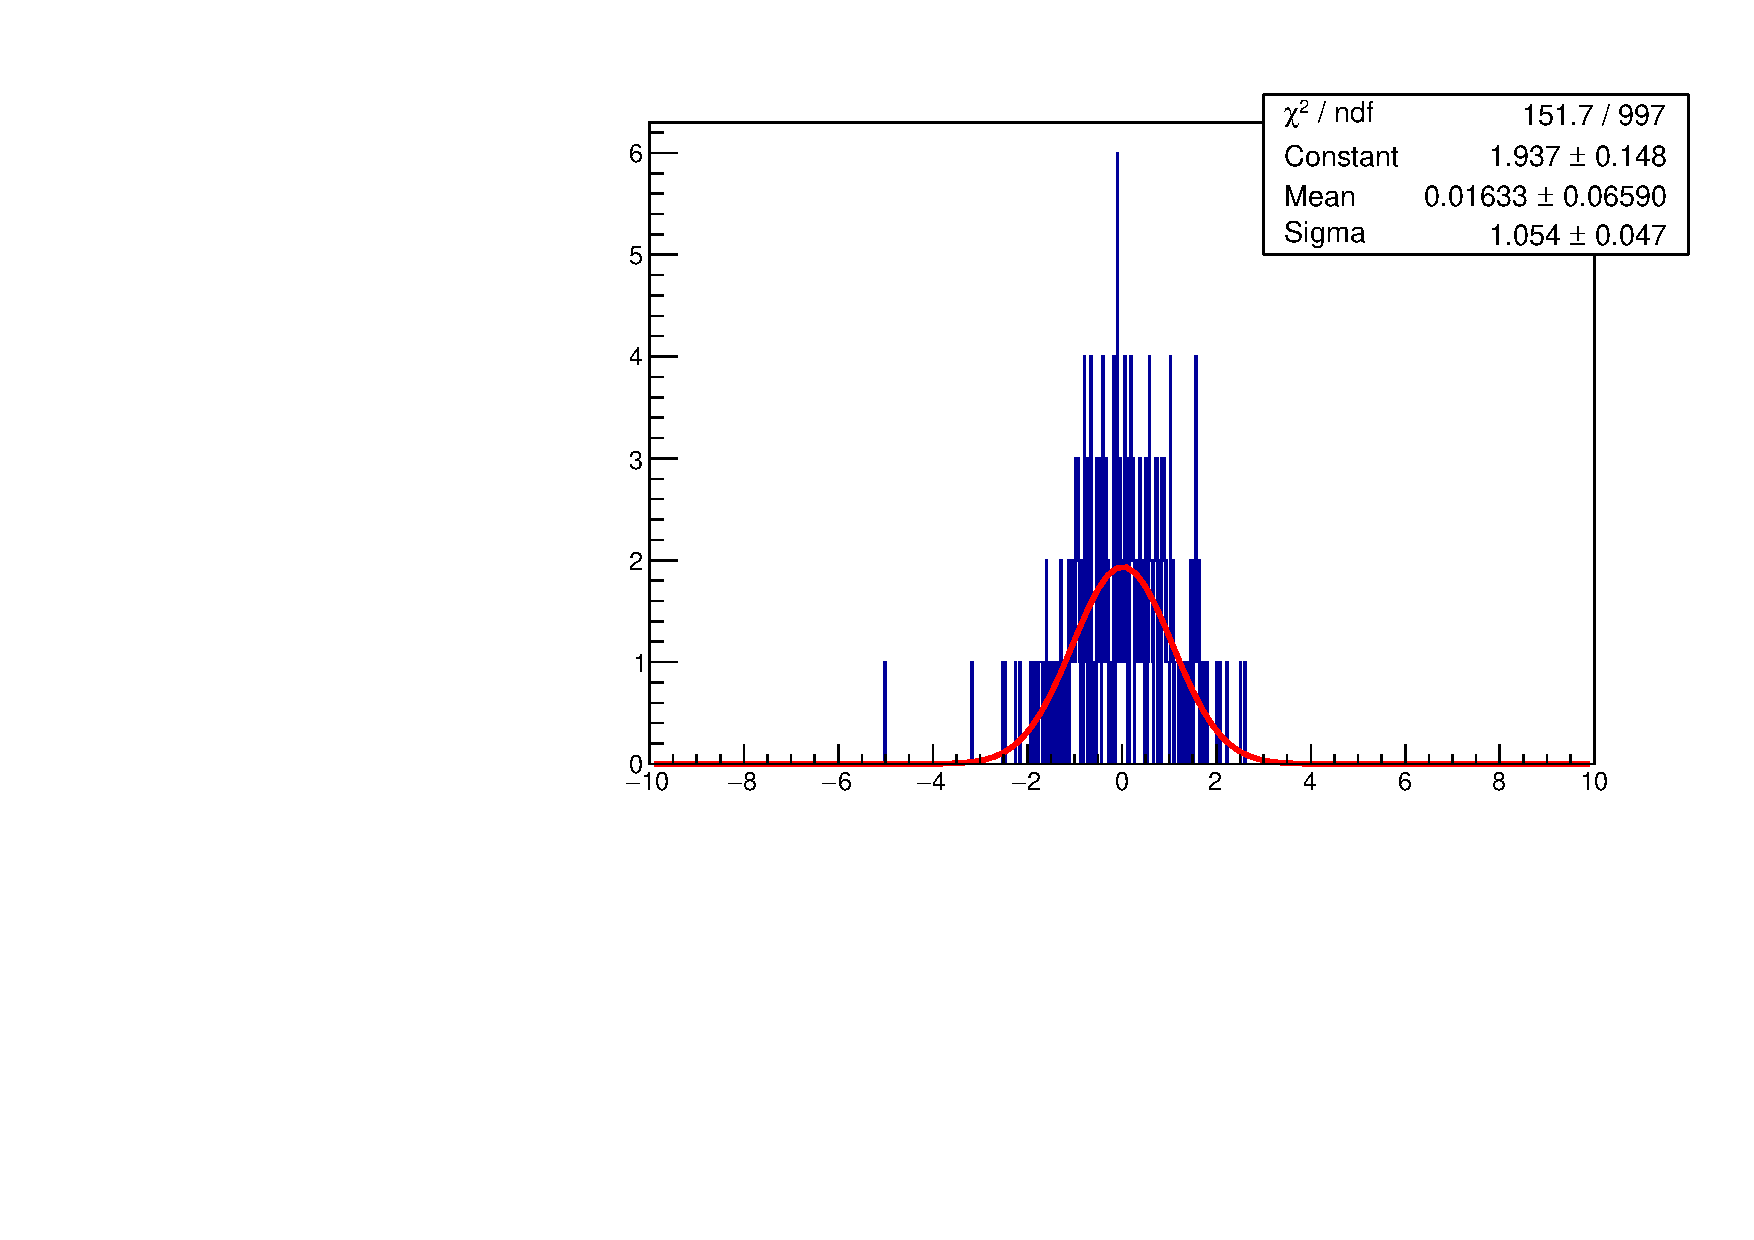
\includegraphics[width=0.45\textwidth]{Figures/03_Zcs/06_Amplitude/noX_plots/new_pull_norminal_2.pdf}
\put(-60,28) {\textrm{\small \bf(a)}}
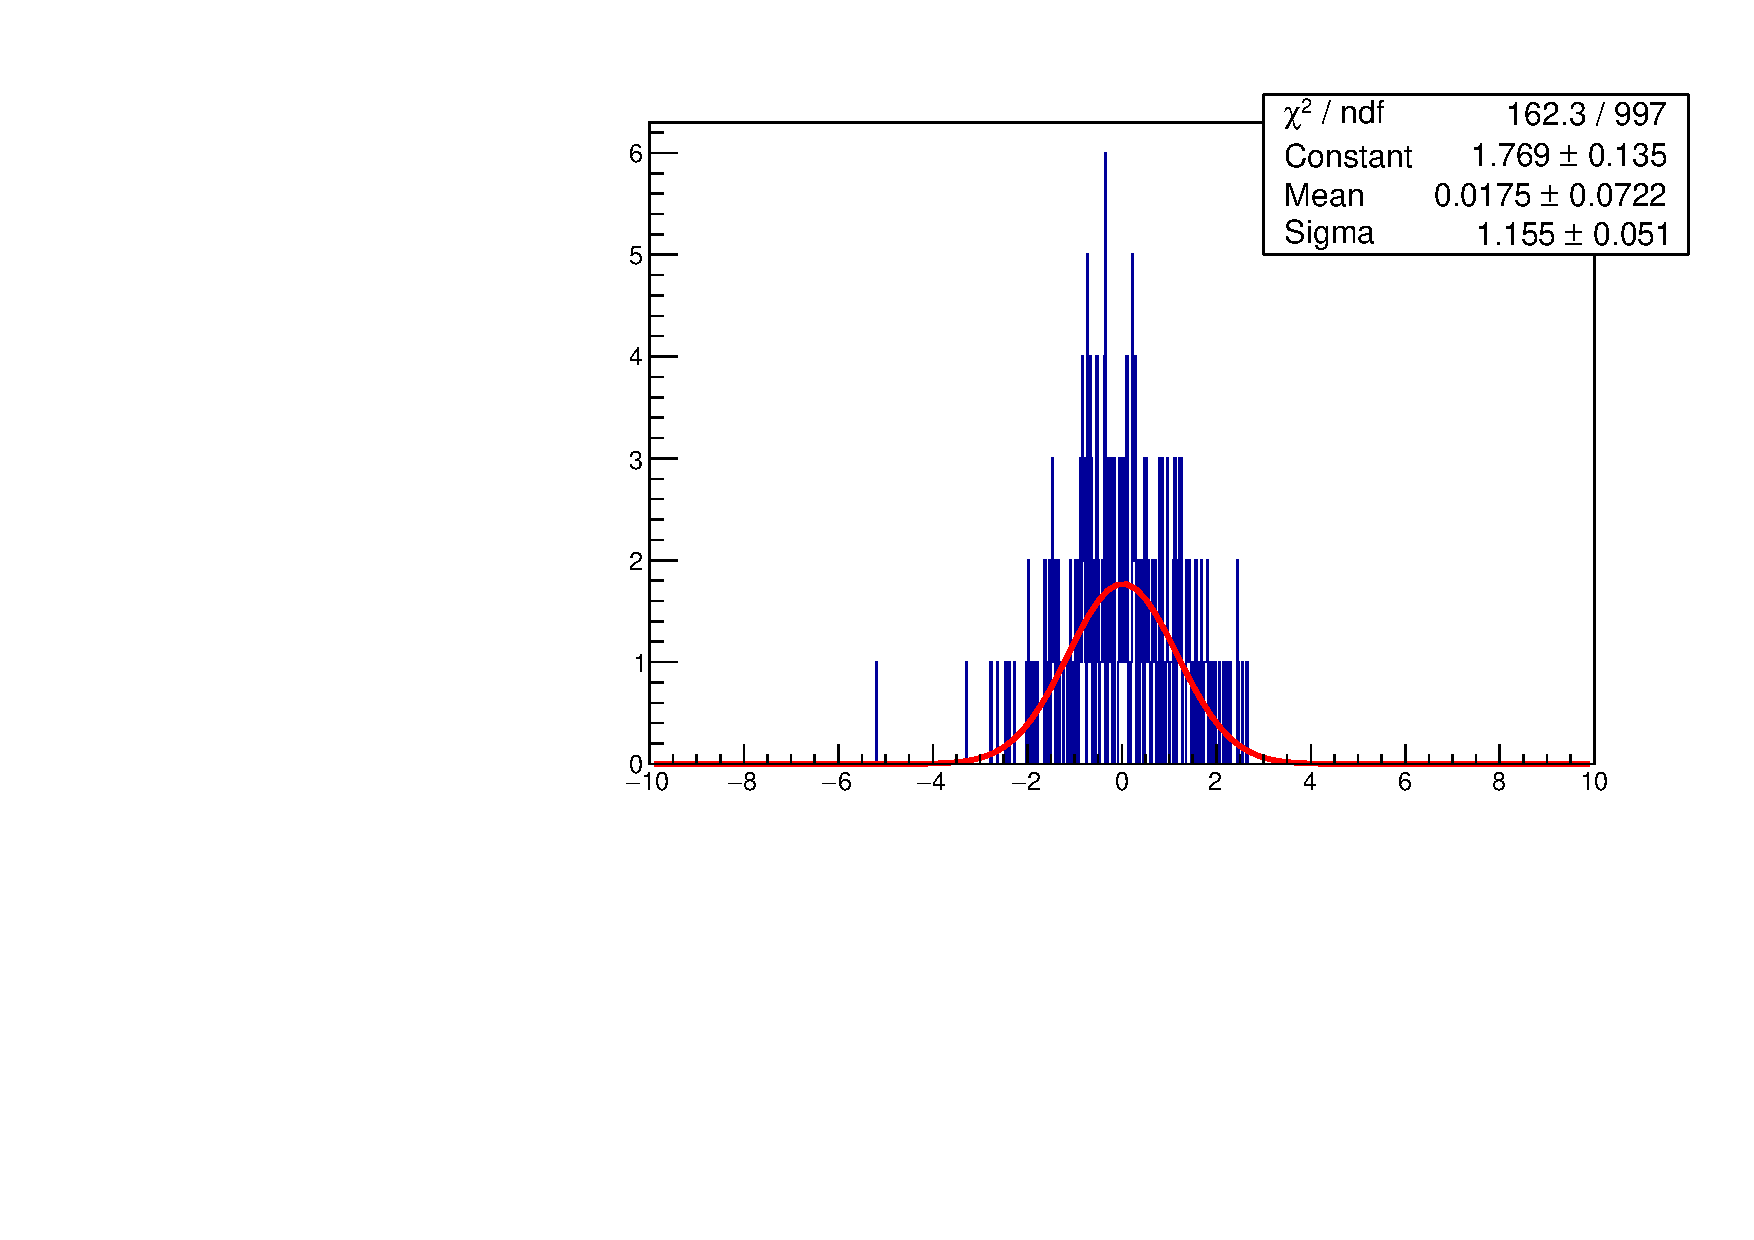
\includegraphics[width=0.45\textwidth]{Figures/03_Zcs/06_Amplitude/noX_plots/new_pull_noX_2.pdf}
\put(-60,28) {\textrm{\small \bf(b)}}\\
\caption{The pull distributions of $\chisq_{2D}$ value in Figure.~\ref{fig:chisq2d},
   The RMS of the pull distribution is smaller when additional $X$ components are introduced. }
\label{fig:rebin_chisq2d_pull}
\end{figure}



\subsection{Flatt\'e function for the $\Xone$ and $Z_{cs}(4000)$ components}
\label{sec:flatte}

As demonstrated in Appendix \ref{SUPPsec:threshold}, 
only $X(4140)$ and $Z_{cs}(4000)$ peak not far from the coupled-channel thresholds of right $J^P$ values in S-wave (higher angular momenta are suppressed for threshold effects). 
In this section,
possible impact of these thresholds is investigated.

Since $\Xone$ peaks near the $\jpsi\phi$ kinematic threshold, 
decays to lighter particle combinations can have a significant impact on its line shape.
As a $1^+$ state $\Xone$ should easily decay via $S-$wave to $D_s^{*\pm}D_s^{\mp}$ which has the lower mass threshold than $\jpsi\phi$.
As an alternative to our nominal fit, 
in which mass dependence of $\Xone$ width is neglected, 
in this section,
mass-dependent width with both channels included is explored. 
The Breit-Wigner formula $BW(m)$ is replaced by the Flatt\'e model: 
\begin{equation}
{\rm Flatte}_X(m|M_0\,,g_{\jpsi\phi}\,,g_{D_s^*D_s})=\frac{1}{M_0^2-m^2-iM_0(g_{\jpsi\phi}\rho_{\jpsi \phi}+g_{D_s^*D_s}\rho_{D_s^*D_s})},
\label{eq:fl}
\end{equation}
where the parameters $g_i$ are the $\Xone$ coupling constants to channel $i$, 
the phase-space factors $\rho_i=2p_i/m$ are dependent on $m\equiv\mjf$ and on momentum $p_i$ of one of the daughters in channel $i$. 
The $\mjf$ mass projections of the fits with $\Xone$ in the Flatt\'e parameterizations for different models of the other components are shown in Figure.~\ref{fig:flatte}. 
The fit parameters are given in Table~\ref{tab:flatte}.  
In term of fit likelihood, 
Flatt\'e parameterization is better than the constant-width Breit-Wigner function by about $\Delta(2\ln\Like)\sim20$ when the same resonance model is used. 
Since in the Flatt\'e model $p_i$ becomes imaginary below the kinematic threshold, 
the real part of the amplitude pole position is not necessarily equal to $M_0$. 
The pole position $m_{\rm pole}\equiv M_{\rm pole}- i\Gamma_{\rm pole}/2$ is obtained by solving the equation that the denominator 
in Equation.~(\ref{eq:fl}) becomes equal to zero when $m=m_{\rm pole}$. 
The results are also reported in Table~\ref{tab:flatte}. 
The pole of Flatt\'e fit corresponds to the 4th Riemann sheet. 
The $Z_{cs}(4220)$ with $J^P=1^{-}$ and $1^+$ hypotheses give similar fit likelihood and 2D $\chisq$ on Dalitz-plot $m^2_{\jpsi\phi}$ and $m^2_{\jpsi K}$ plane, 
and the fit results with $Z_{cs}(4220)$ in the $1^-$ hypothesis are also shown.
In all Flatt\'e fits, 
the coupling of $X(4140)$ to the coupled-channel is smaller than to the $\jpsi\phi$ and is insignificant. 


\begin{table}[hbtp]
\centering
\caption{Comparison for $\Xone$ resonance with Flatt\'e and constant-width Breit-Wigner functions. 
The numbers between horizontal bands, the first (second), correspond to $Z(4220)$ with $J^P=1^{-(+)}$.  
Also shown are the $\ln\Like$  and 2D $\chisq$ of Dalitz-plot distribution in the $m^2_{\jpsi\phi}$ vs.\ $m^2_{\jpsi K}$ plane with 1018 adaptive bins.}\label{tab:flatte}
\small{
\begin{tabular}{lccccccc}\hline
Flatt\'e&  $M_0$ (MeV)& $g_{\jpsi\phi}$ (GeV)& $g_{D_s^*D_s}/g_{\jpsi\phi}$ & Pole (MeV)&FF (\%)& $\ln\Like$& 2D $\chisq$\\\hline
Nominal & $  4202 \pm    18 $ & $  1.44 \pm  0.36 $ & $  0.05_{-0.05}^{+0.40} $  & $4092 - 90 i$ & $  19.1 $ &  5012.0 & 1022\\
Nominal & $  4223 \pm    29 $ & $  1.61 \pm  0.48 $ & $  0.06_{-0.06}^{+0.40} $ & $4082 - 113 i$ & $  17.7 $ &  5013.1 & 1039\\ 
\hline
Extended & $  4216 \pm   23 $ & $  1.46 \pm  0.44 $ & $  0.10_{-0.10}^{+0.40} $ & $4089 - 108 i$& $  35.3 $ &  5080.1 & 1001\\ 
Extended & $  4187 \pm   22 $ & $  1.06 \pm  0.49 $ & $  0.34_{-0.28}^{+0.40} $ & $4084 - 83 i$& $  21.0 $ &  5074.4 & 1027\\ 

\hline\hline
BW&  $M_0$ (MeV)& \multicolumn{2}{c}{$\Gamma$ (GeV)}& Pole (MeV) &FF (\%)& $\ln\Like$  & 2D $\chisq$\\\hline
Nominal & $  4116\pm 10 $ & \multicolumn{2}{c}{$   130 \pm 21 $} & $  4116 -    65 i $ & $  18.0 $ &  5001.6 & 1028\\ 
Nominal & $  4118\pm 14 $ & \multicolumn{2}{c}{$   162 \pm 22 $} & $  4118 -    81 i $ & $  17.4 $ &  5004.6 & 1044 \\ \hline
Extended & $  4107\pm 12 $ & \multicolumn{2}{c}{$   168 \pm 21 $} & $  4107 -    84 i $ & $  43.2 $ &  5070.4  & 1004\\ 
Extended & $  4108\pm 12 $ & \multicolumn{2}{c}{$   137 \pm 22 $} & $  4108 -    69 i $ & $  21.0 $ &  5068.7 & 1029\\ 
 
\hline
\end{tabular}
}
\end{table}

\begin{figure*}[t]
\centering
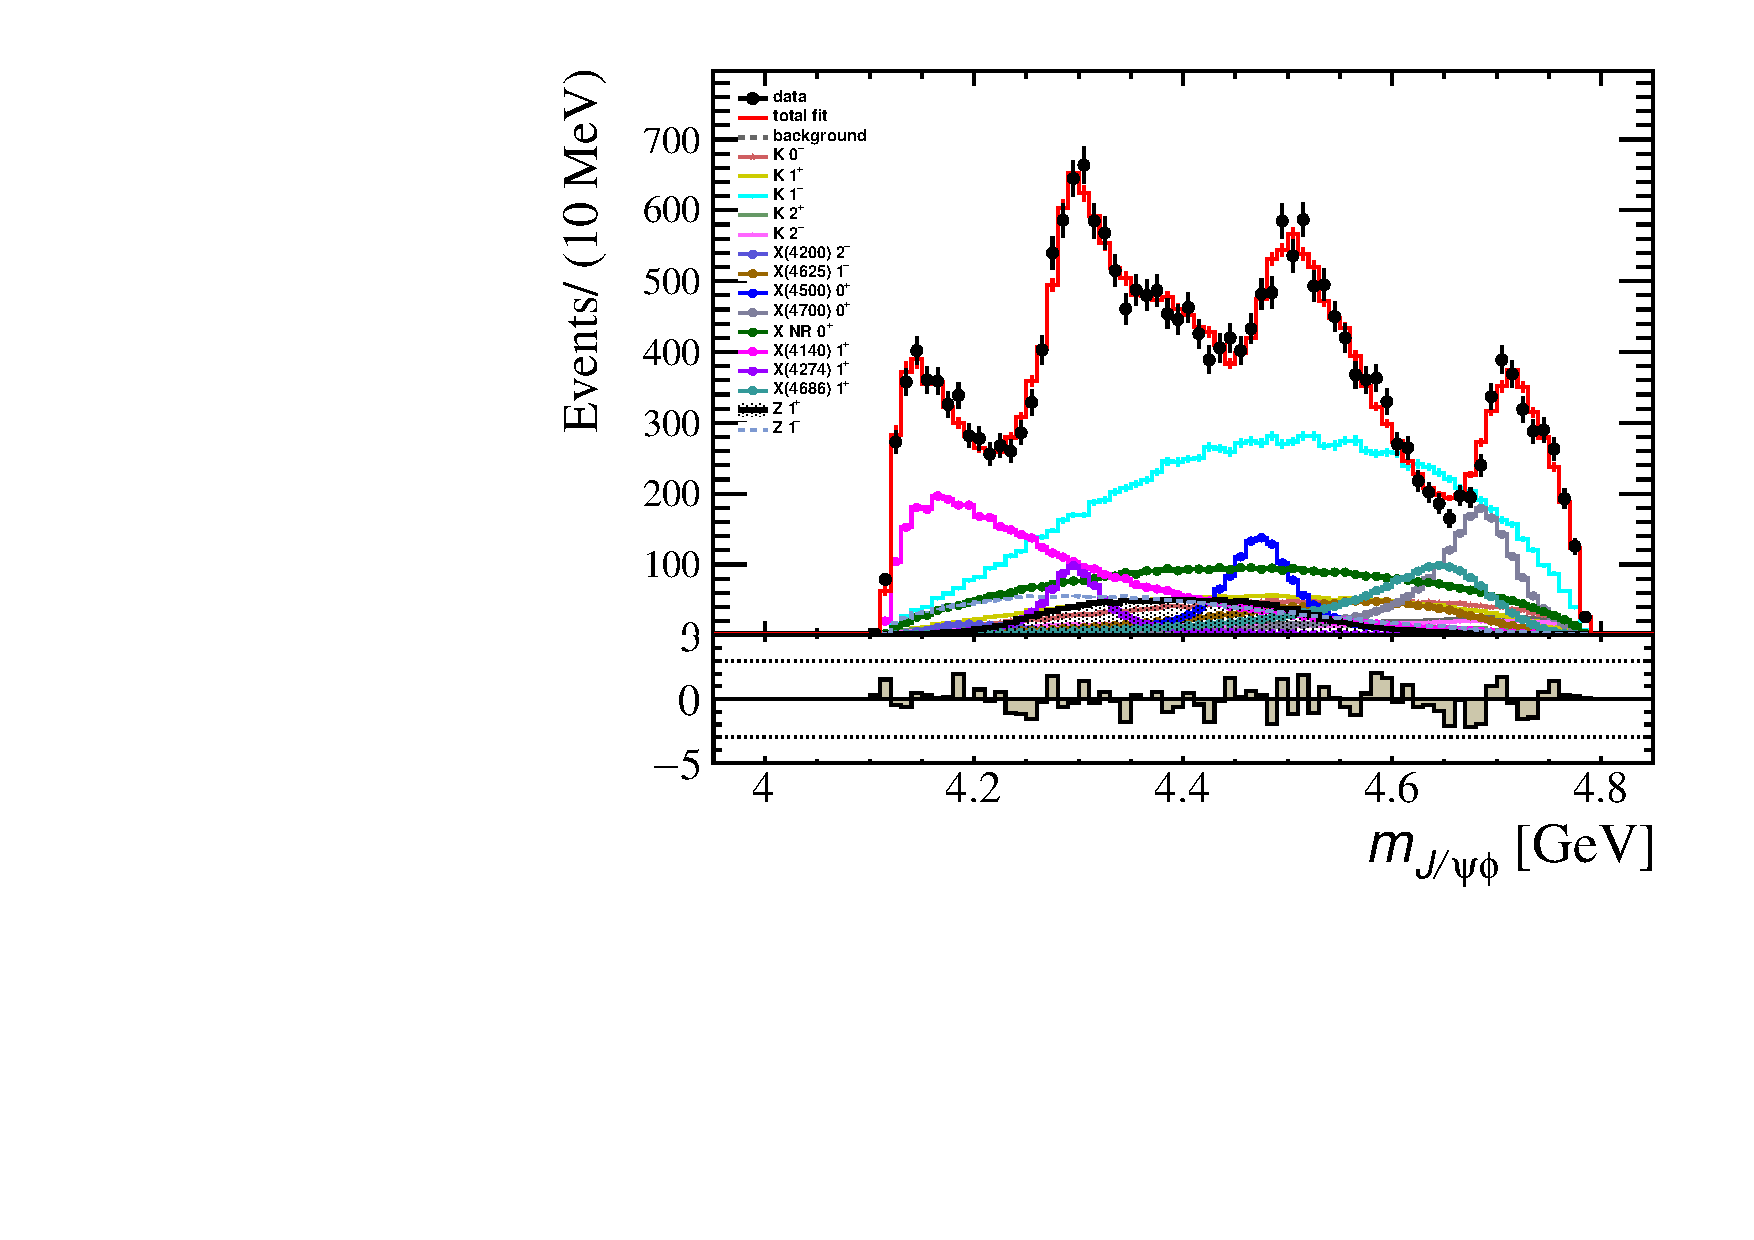
\includegraphics[width=0.5\textwidth]{Figures/03_Zcs/06_Amplitude/Flatte/mjpsiphi-4140FL-Z1M}%
\put(-50,140) {\textrm{\small \bf(a)}}%
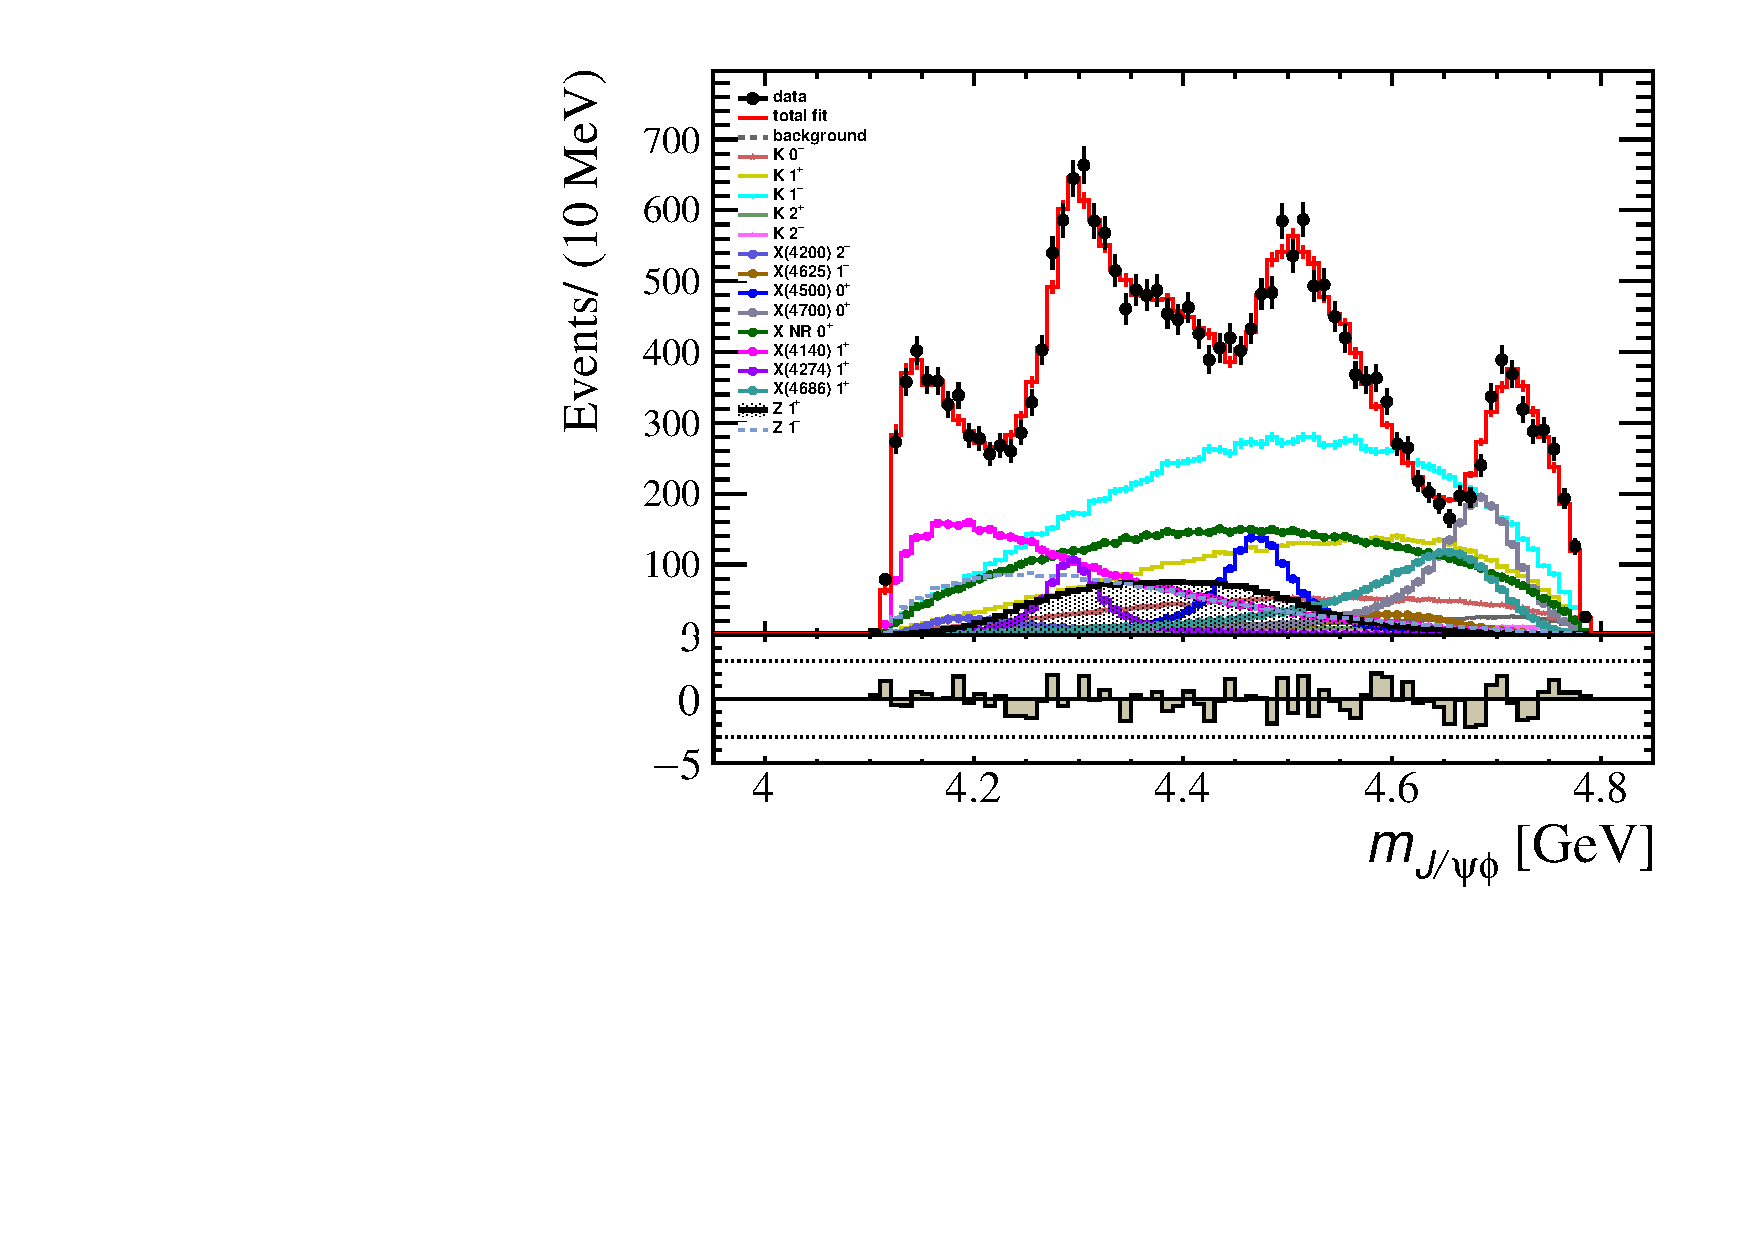
\includegraphics[width=0.5\textwidth]{Figures/03_Zcs/06_Amplitude/Flatte/mjpsiphi-4140FL-Z1P}
\put(-50,140){\textrm{\small \bf(b)}}\\
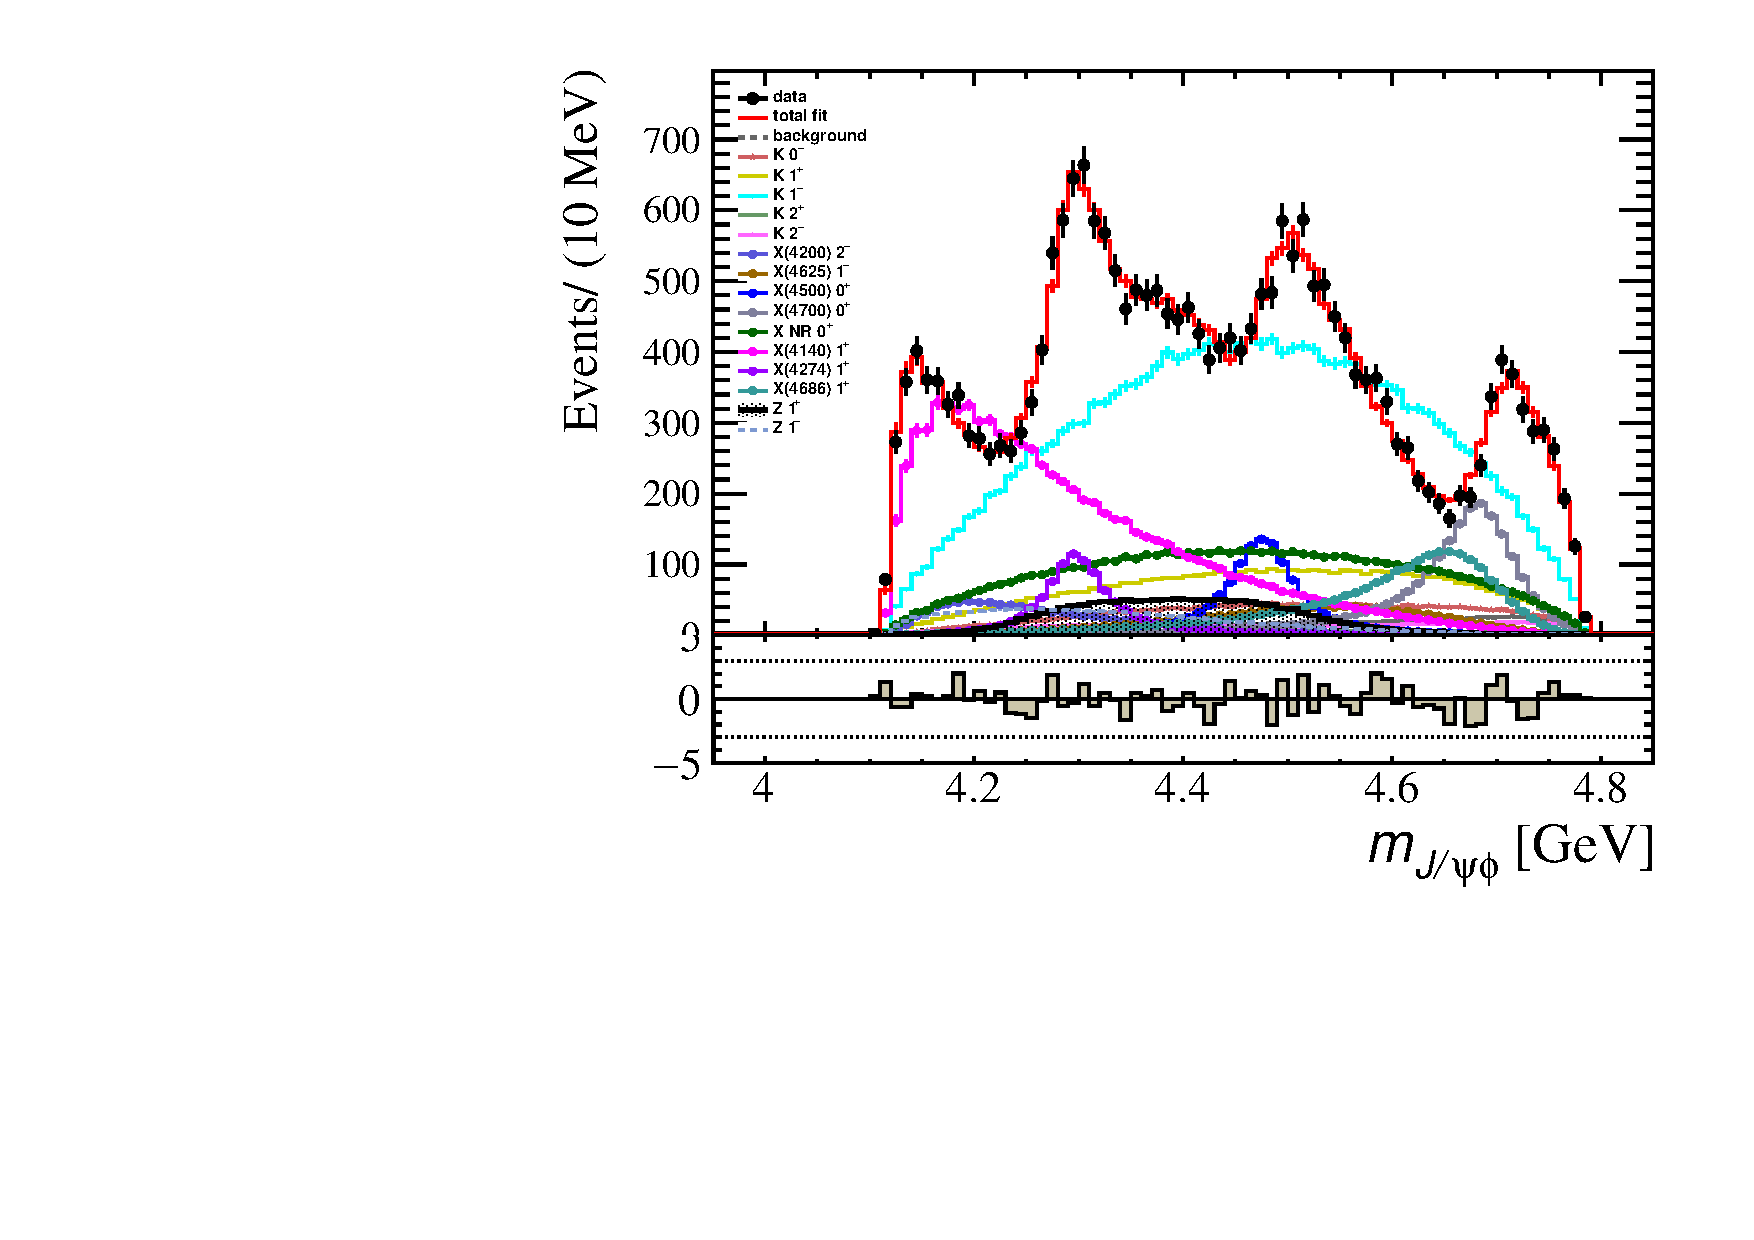
\includegraphics[width=0.5\textwidth]{Figures/03_Zcs/06_Amplitude/Flatte/mjpsiphi-AllKFL-Z1M}%
\put(-50,140) {\textrm{\small \bf(c)}}%
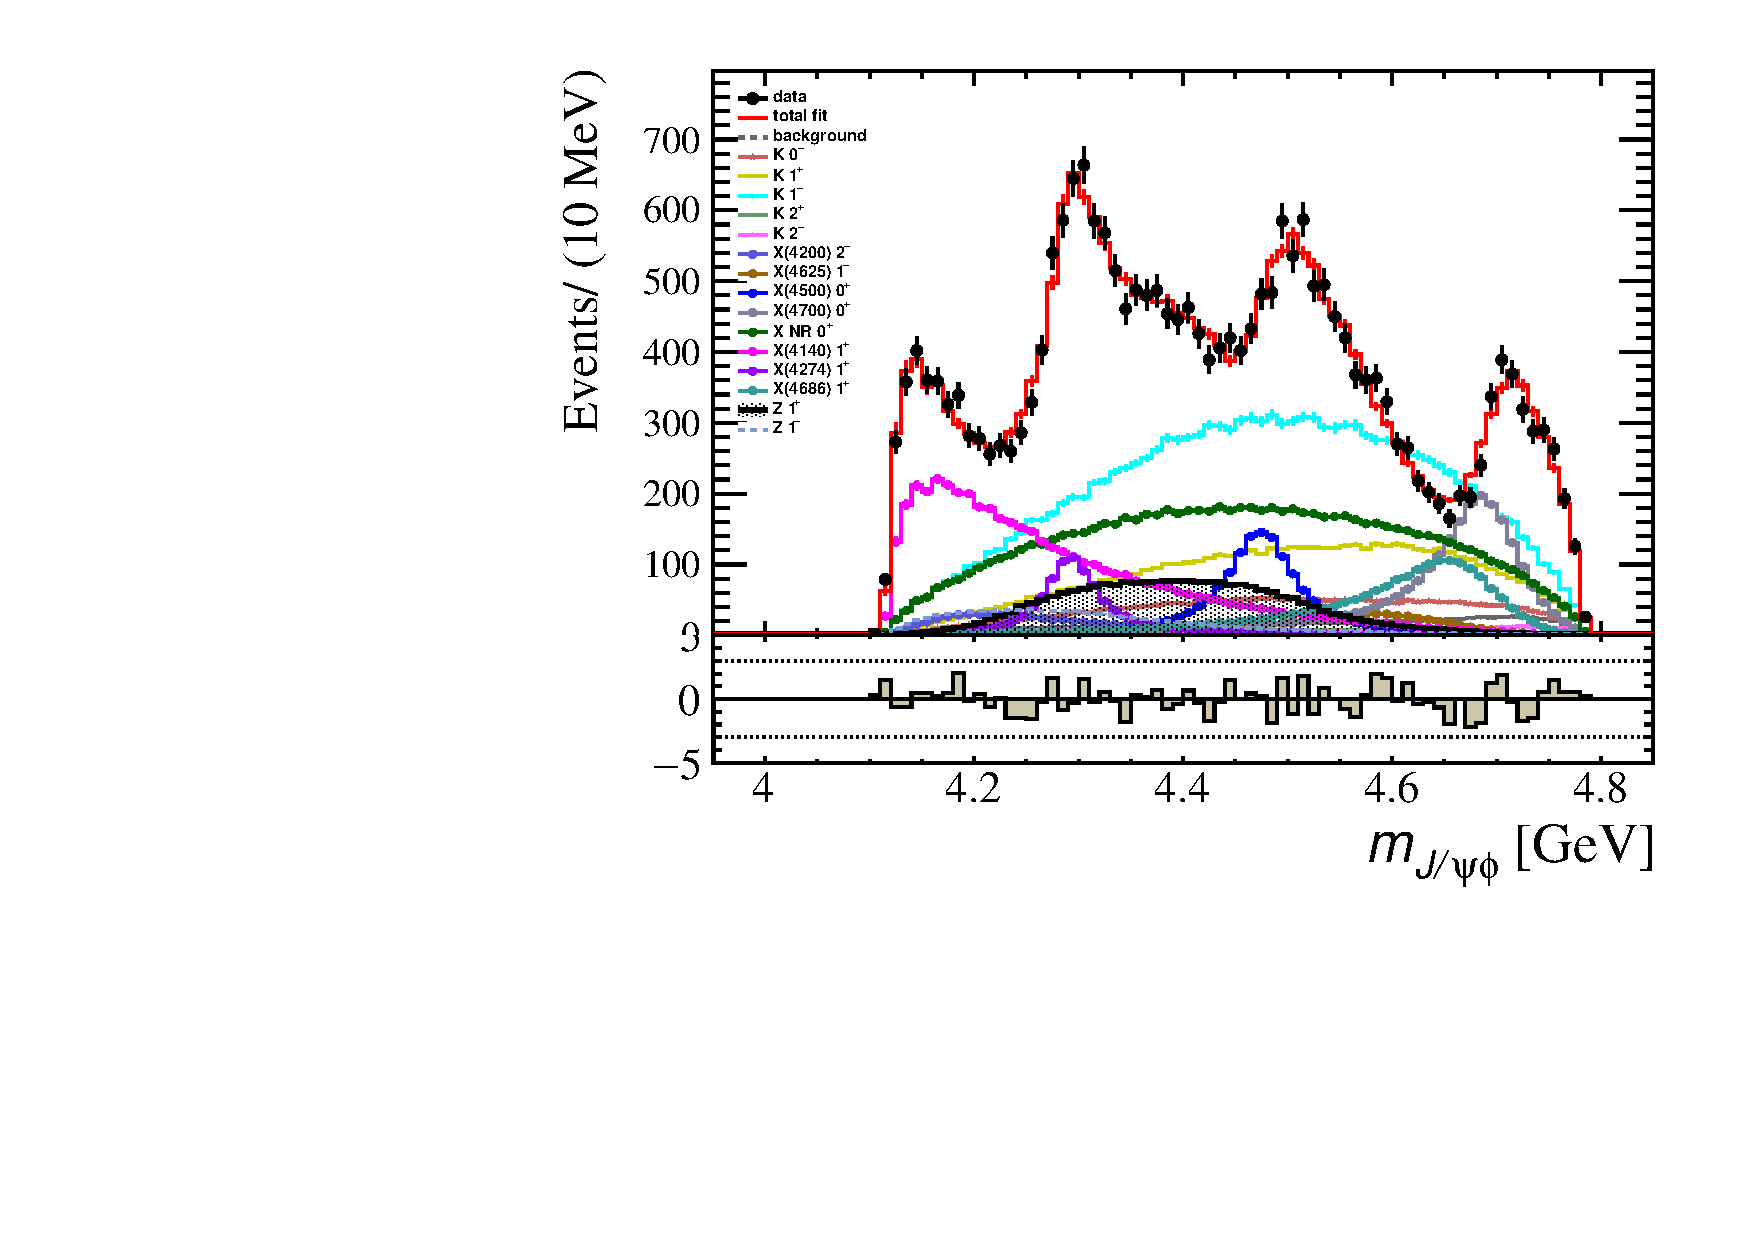
\includegraphics[width=0.5\textwidth]{Figures/03_Zcs/06_Amplitude/Flatte/mjpsiphi-AllKFL-Z1P}
\put(-50,140){\textrm{\small \bf(d)}}
\caption{Projections of $\mjf$ from fits of Flatt\'e function for describing $\Xone$ in different resonance models 
(a) nominal $K$ and $1^-$ $Z(4220)$, (b) nominal $K$ and $1^+$ $Z_{cs}(4220)$, (c) extended $K$ and $1^-$ $Z_{cs}(4220)$, (b) extended $K$ and $1^+$ $Z(4220)$.}
\label{fig:flatte}
\end{figure*}

\begin{figure}[bt]
\centering
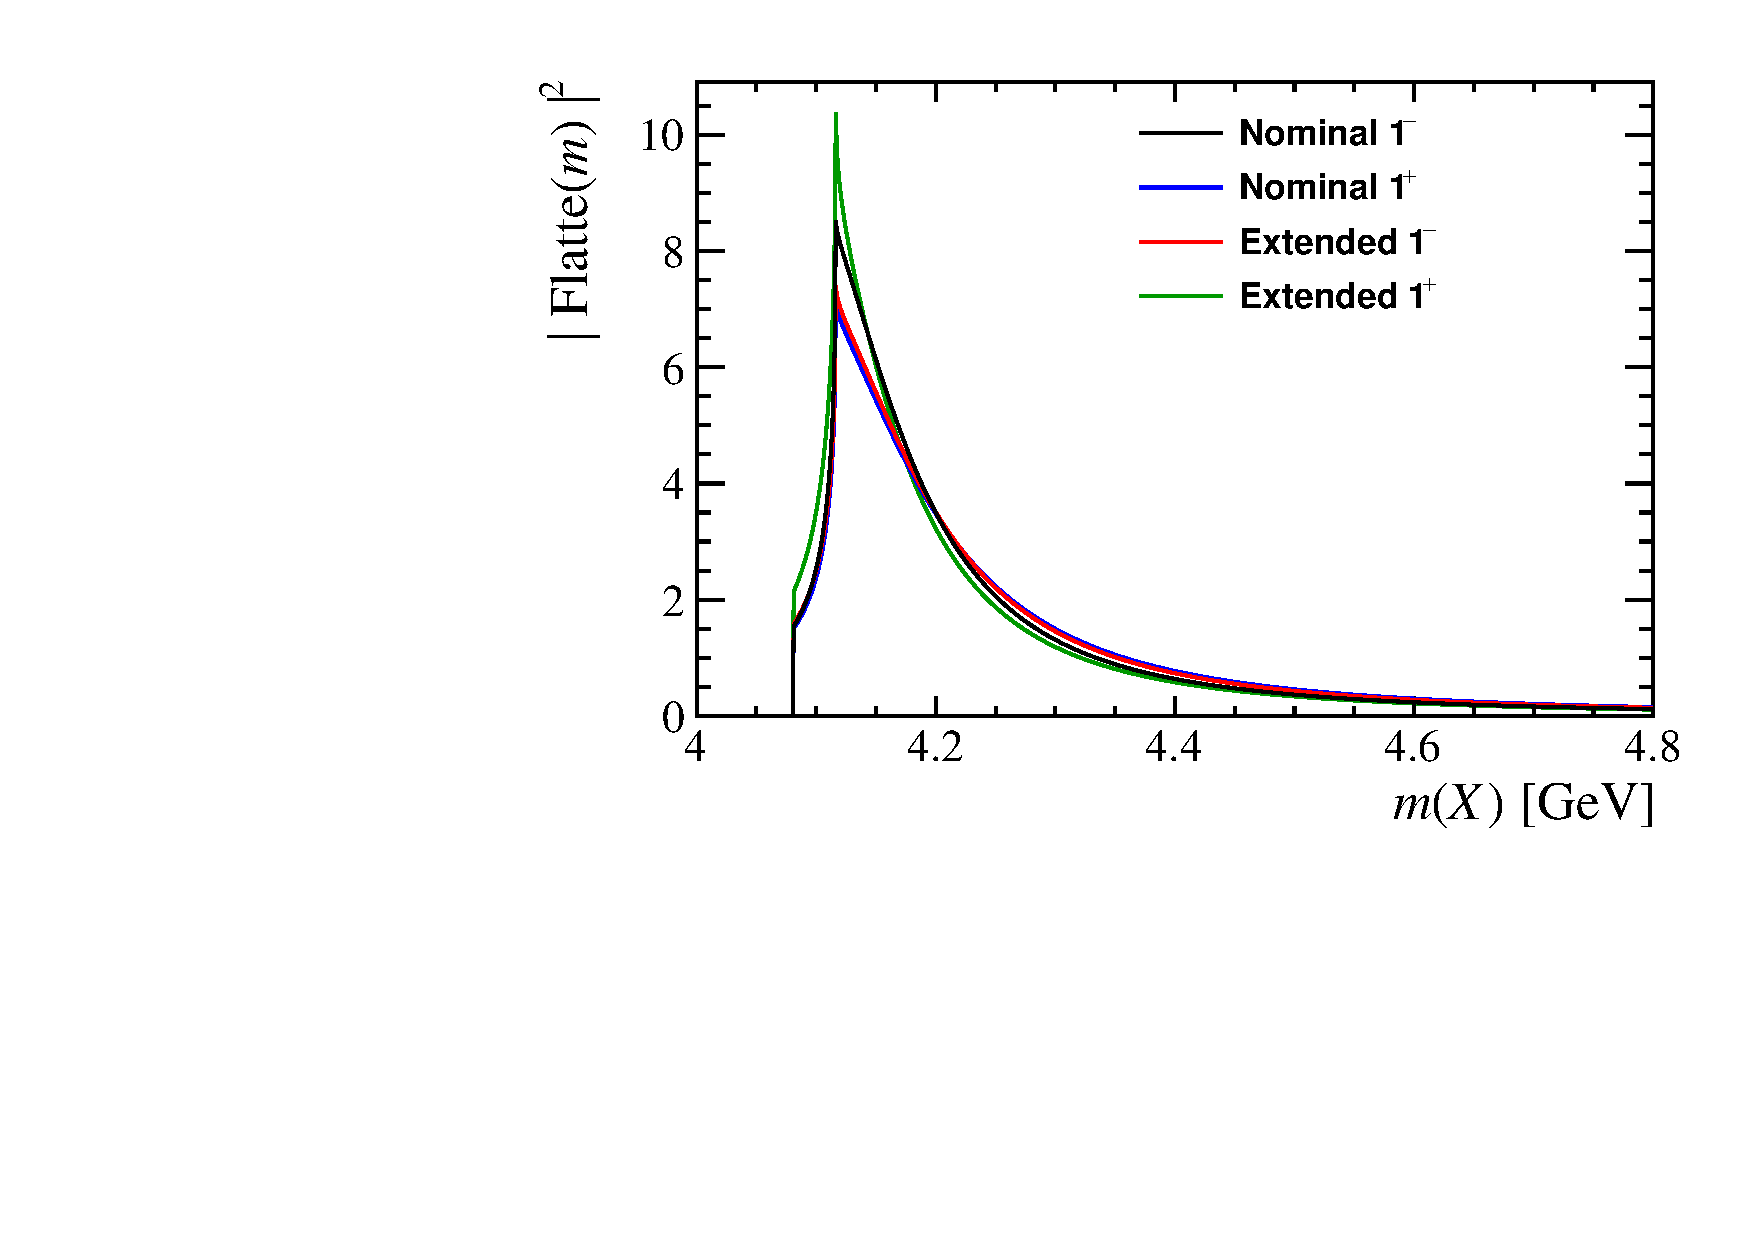
\includegraphics[width=0.65\textwidth]{Figures/03_Zcs/06_Amplitude/Flatte/FlatteX}
\caption{Lineshapes of Flatt\'e parameterization of the $\Xone$ resonance.}\label{fig:cmpfl}
\end{figure}


The Flatt\'e $\Xone$ lineshapes, moduli of Eq.~(\ref{eq:fl}) squared, 
are compared in Figure.~\ref{fig:cmpfl}. 
Without the phase-space factor of $X\to\jpsi \phi$ decays, 
the lineshapes peak at the threshold. 
Similar results are obtained with the Breit-Wigner parameterization using constant width. 

Using Flatt\'e for $Z_{cs}(4000)^+$ is also investigated since it peaks close to the mass threshold of $\Dsp \Dstarzb$ and $\Dssp\Dzb$, 
assuming the same couplings for the two open charm channels. 
Also note that when $\mjk$ is below the mass threshold of one of the coupled channels, 
the channel's phase space factor becomes imagery. 
The fit is slightly better, $\Delta(-2\ln\Like)=2.8$,
but the improvement is not significant given that there is one addition free parameter in this model.
The fit results are $M^F_0=4029\pm22\mev$, $g_{\jpsi\Kp}=0.38\pm0.07\gev$, $(g_{\Dsp \Dstarzb}+g_{\Dssp\Dzb})/g_{\jpsi\Kp}=0.8\pm0.6$. 
While the coupling to $\jpsi\phi$ is significant, 
the coupling to the coupled-channels is not. 
However, within the large errors it is possible that the threshold plays an important role.
A pole for $Z_{cs}(4000)^+$ in Flatt\'e representation is found to be $M_0-i\Gamma_0/2=(4004\pm12 -i 91\pm22)$\mev. 
The statistical uncertainties are calculated by toy study where the correlations of the three parameters in Flatt\'e function are taken into account. 
The projection of this fit onto $\mjk$ is shown in Figure.~\ref{fig:FlatteZcs}.

\begin{figure*}[t]
\centering
%\begin{minipage}[b]{0.5\textwidth}
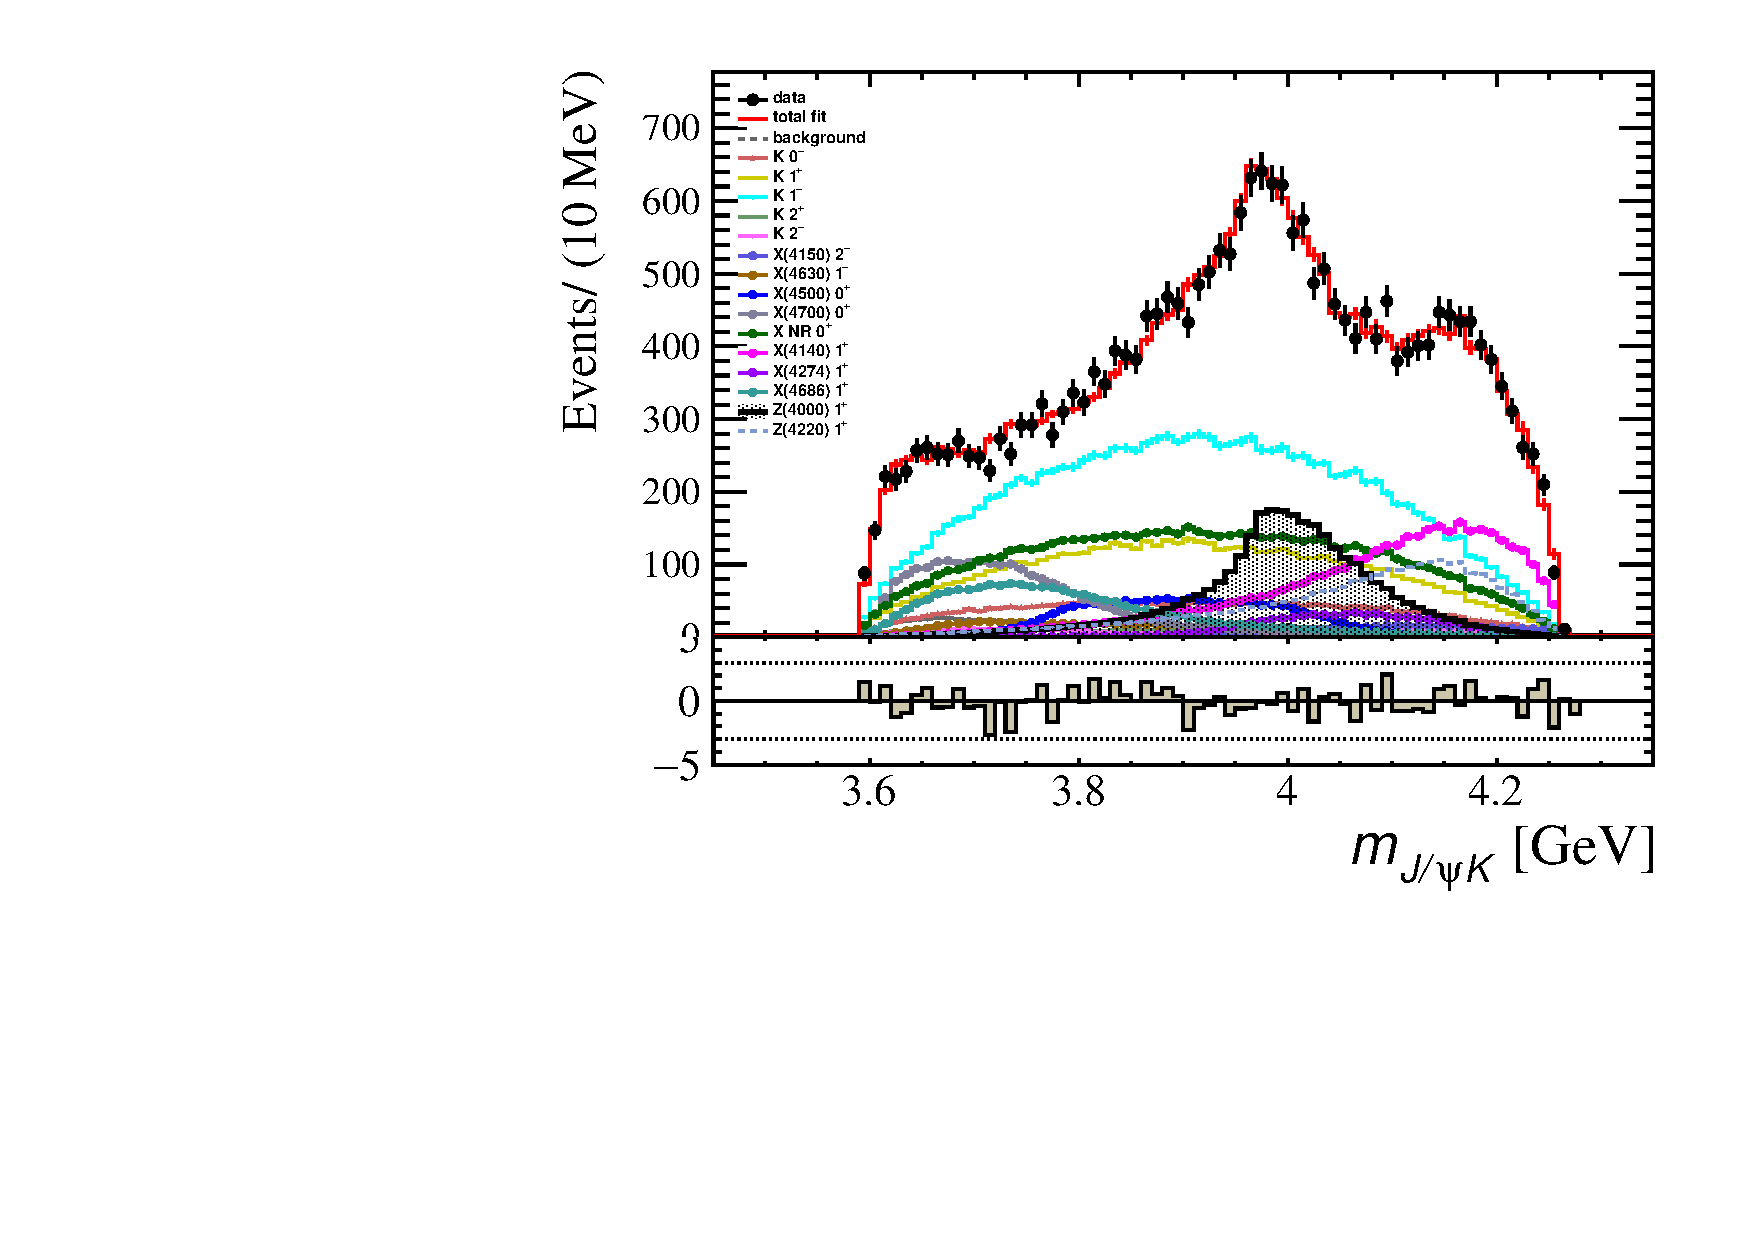
\includegraphics[width=0.6\textwidth]{Figures/03_Zcs/06_Amplitude/Flatte/mjpsik-Z1PZFL}%
\caption{Projections onto $\mjk$ from the fit with the Flatt\'e function for describing $Z_{cs}(4000)^+$.}
\label{fig:FlatteZcs}
\end{figure*}








